\documentclass[parskip=half, twoside=false]{scrreprt}
\usepackage{lmodern}
\usepackage[utf8]{inputenc}
\usepackage{natbib}
\usepackage{graphicx}
\usepackage{url}
\usepackage{verbatim}
\usepackage{siunitx} %For degree symbol etc.
\DeclareSIUnit\bar{bar}
\usepackage[table,xcdraw]{xcolor}
\usepackage{geometry} %packages für gescheite A4 Seite
\usepackage{lscape} %to have tables in landscape mode
\usepackage{float} %to place figures where they are in the source with [H]
\usepackage{pdfpages} %to insert pdfs for appendices
\usepackage[caption = false]{subfig}
\restylefloat{table} %makes [H] possible for tables as well
\setcounter{secnumdepth}{4}

\geometry
{
	paper					=	{a4paper},
	ignoreheadfoot,
	hmargin					=	{20mm},
	vmargin					=	{25mm},
	headsep					=	{5mm},
	footskip				=	{\dimexpr5mm+\normalbaselineskip},
	headheight		    	=	{10mm},
}
\usepackage{hyperref}
\usepackage{cleveref}

\newcommand{\uH}{$\mu$Houbolt }

\title{\boldmath{$\mu$}Houbolt Technical Report}
\subtitle{Team 25 Technical Report to the 2022 EuRoC}
\author{TU Wien Space Team}
\date{2022}

\begin{document}

\maketitle

\newpage

\tableofcontents

\newpage

\chapter{Abstract}
\label{chap:abstract}

\uH is a bi-liquid propelled rocket project by the TU Wien Space Team. Designed and manufactured almost exclusively in-house, with the needed Know-How slowly built up over precursor projects and the projects life cycle, the team has managed to create a robust and lightweight rocket together with the necessary Testing and Ground Support Equipment to safely operate it.

The rocket is designed to fly to an altitude of \SI{3}{\kilo\meter} - thus being in the L3 launch category - using its engine powered by ethanol and liquefied nitrous oxide and to then safely return to the ground thanks to a two stage recovery system. The engine design has been iterated upon over years with many improvements on every part from the injector over propellant feed pressures and igniters to combustion chamber concepts. Throughout the entire project special care has been put into safety, ranging from refining checklists to be as clear as possible, over a remote controlled oxidizer loading system to bleed orifices and burst discs for passive depressurization. As liquid rockets need a lot more and more complex Ground Support Equipment than a typical solid propelled rocket, considerable amount of time has also been invested in simple and easy to use Mission Control software that can control both the rocket while on the pad and the GSE.

The payload flown will be the EDU subsystem from the STS1 (SpaceTeamSat1) project from Space Team. This gives the cubesat project the opportunity to flight test parts of their hardware.

\newpage

\chapter{Introduction} %Luis

TU Wien Space Team is a student organization engaging in various projects in aerospace engineering. Our mission statement is to foster the Know-How and enthusiasm for aerospace technologies in our peers by providing an accessible entry into rocketry and giving members the opportunity to learn. The team is working on a number of different projects ranging from solid propelled two staged rockets, which can reach the edge of space to hydrogen powered autonomous airplanes and from cubesats to rockets with liquid propulsion systems.

The \uH project has its origin as a small scale technology demonstrator for our large rocket concept, Houbolt. The much reduced scale has allowed for faster and cheaper iteration in development and testing and has given us the opportunity to gather experience and work on our testing equipment and ground infrastructure. The goal of the project is to build and launch the first bi-liquid propelled rocket of the Space Team. The design should provide a solid foundation which can be further developed and used in more advanced projects. If regulatory limitations allow it, we would like to make the design open-source after a successful launch at EuRoC.

Our mission objectives are as follows:
\begin{itemize}
    \item Flight to target altitude of \SI{3}{\kilo\meter}
    \item Successful 2-stage recovery of vehicle
    \item Working telemetry and data recording during the whole mission
    \item Secondary mission: test platform for the CubeSat project STS1 from Space Team
\end{itemize}

\section{Academic Program} %Liana
The TU Wien Space Team is a student association with about 250 members. Due to the affiliation to the TU Wien and the technical focus of the projects, the team consists largely of students from the TU Wien and the fields of study Mechanical Engineering, Electrical Engineering, Technical Physics and Computer Science.
However, efforts are being made to make the team more diverse and to include students from other universities and fields of study. As a result, we now have students from e.g. the University of Vienna, the Vienna University of Economics and Business Administration, the University of Applied Sciences St. Pölten, the University of Applied Arts Vienna and University of Applied Sciences Wiener Neustadt in our team.

\section{Stakeholders}
Apart from universities, which gain visibility and reputation through TU Wien Space Team, and students, who have the opportunity to deepen their knowledge and apply it in practice, there are other parties that are essential for the organisation.
Industry sponsors provide resources and mentor the team members, for example by sharing manufacturing techniques or holding workshops. In return, the project provides visibility both internally to highly motivated students with practical experience and with that to possible future employees and externally to potential customers.

\section{Team Structure} %Liana
TU Wien Space Team is divided into eight active projects:
\begin{itemize}
\item The Hound: Two staged solid rocket slated to reach the Karman Line
\item \uH: Bi-liquid propelled rocket
\item SpaceTeamSat1: Fully in-house developed and built cubesat
\item GATE: Large scale liquid propellant engine
\item AcrossAustria: Hydrogen-powered long range autonomous drone
\item Penrose: Hybrid rocket
\item CanSat: Space Team as launch provider for student-built can-sized satellites
\item FIRST: Onboarding project for new Space Team members as an introduction to rocketry
\end{itemize}
In addition, there are organisational and cross-project departments, those being IT, HR, finance and marketing.

\subsection{\uH Team Structure} 
Currently, about 25-30 people are working on project \uH. Although the structures are flat and exchange across the team is encouraged, there are clearly assigned tasks and module leads who are responsible for ensuring that the goals in their respective areas -- these being Recovery, Propulsion, Avionics, Ground Systems, Aerostructure and Software -- are achieved. Additionally, internal module meetings are held weekly to assign and discuss tasks. 

The workload of the team members is rather diverse: while a minimum of 5 hours per week is expected of everyone, active members devote all their available time into the project at stressful phases. Being able to choose the effort so freely allows us to have a diverse team, whereby the willingness to put time and energy into the project is naturally reflected in the weight of the tasks and the position in the team structure.
Apart from that, the team can draw on the experience of former members, who are consulted when questions arise, that have already been dealt with in previous projects.

In addition to the members who work on the rocket directly, there are people within the team who take care of the project's presence on social media, photography and legal matters.

\section{Technical Challenges}
A considerable challenge was to not only build a liquid propulsion system from the ground up, but to also make it as small and lightweight as we did. Eliminating parts is always good for eliminating risks and reducing weight is obviously a positive impact for rocket performance, but that is easier said than done. Additionally we've put a lot of effort into the safety of our design, both by designing systems that are easy to operate and having as little interaction with hardware that is in a potentially harmful state as possible by remote controlling large parts of the ground support equipment.
A compounding factor for all this is that the entire software stack has been designed and developed completely in-house without using external software solutions (excluding CAN driver and the used Operating Systems) - the same goes for mechanical components, which we tried to manufacture in our own workshop safe for the aluminium propellant tanks, some of the plumbing \& valves and the main carbon fiber body tube.

\section{Vision} %Liana
The team's vision is that \uH will become a benchmark for bi-liquid rockets in the field of student rocketry. The entire project should go open source, and thus provide the foundation for further development. The advantages \uH has already had for us -- fast and cost-efficient iteration thanks to small scale and well thought-out designs -- should be of advantage to future rocket enthusiasts.


\newpage

\chapter{System Architecture}
\label{chap:sysarch}

\section{Overview}

\subsection{Physical Architecture}
\Cref{fig:sysarch_cad} shows a rendering of the \uH CAD model. The vehicle consists of the airframe, the propulsion system, the recovery system and avionics. The propulsion system structure, which also contains the avionics components, is self-contained and can be slid into the airframe from the bottom. The recovery system is mounted to the top of the airframe. The custom pressure bearing components were validated using FEM simulations as well as pressure proof tests to 1.5x of maximum pressure.

\begin{figure}[h]
    \centering
    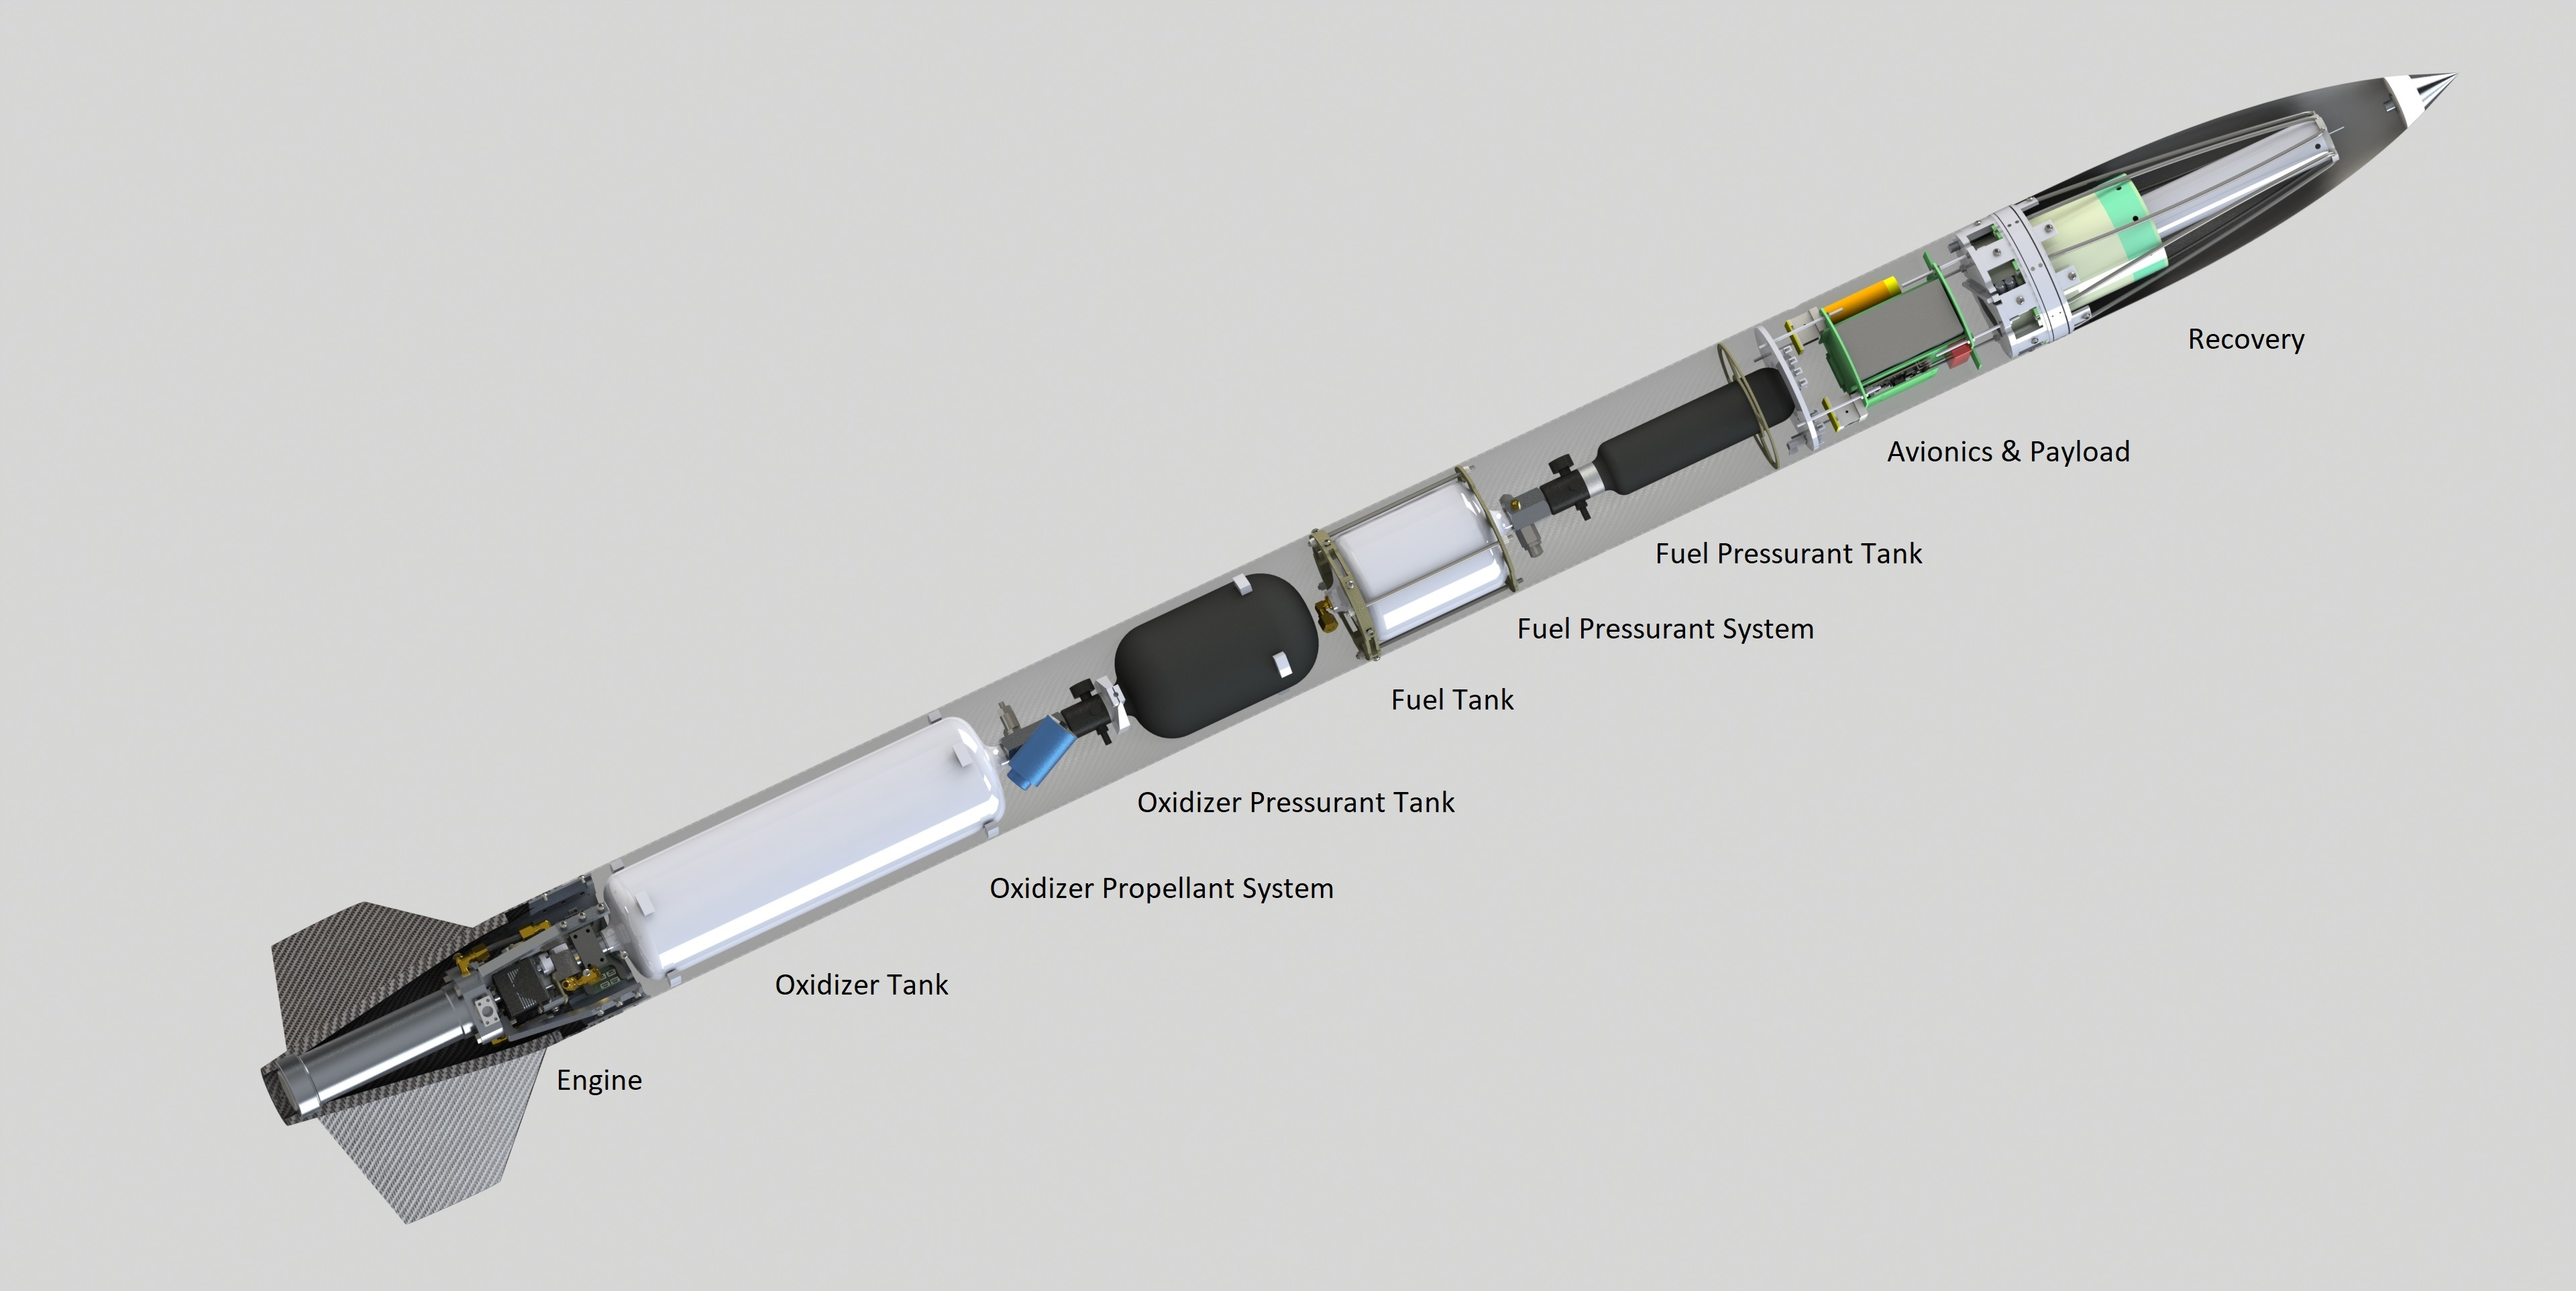
\includegraphics[width=\textwidth]{SysArch/uHb_render.jpg}
    \caption{\uH physical architecture}
    \label{fig:sysarch_cad}
\end{figure}

\subsection{Fluid System}\label{sec:sysarch_fluidSystem}

\begin{figure}
    \centering
    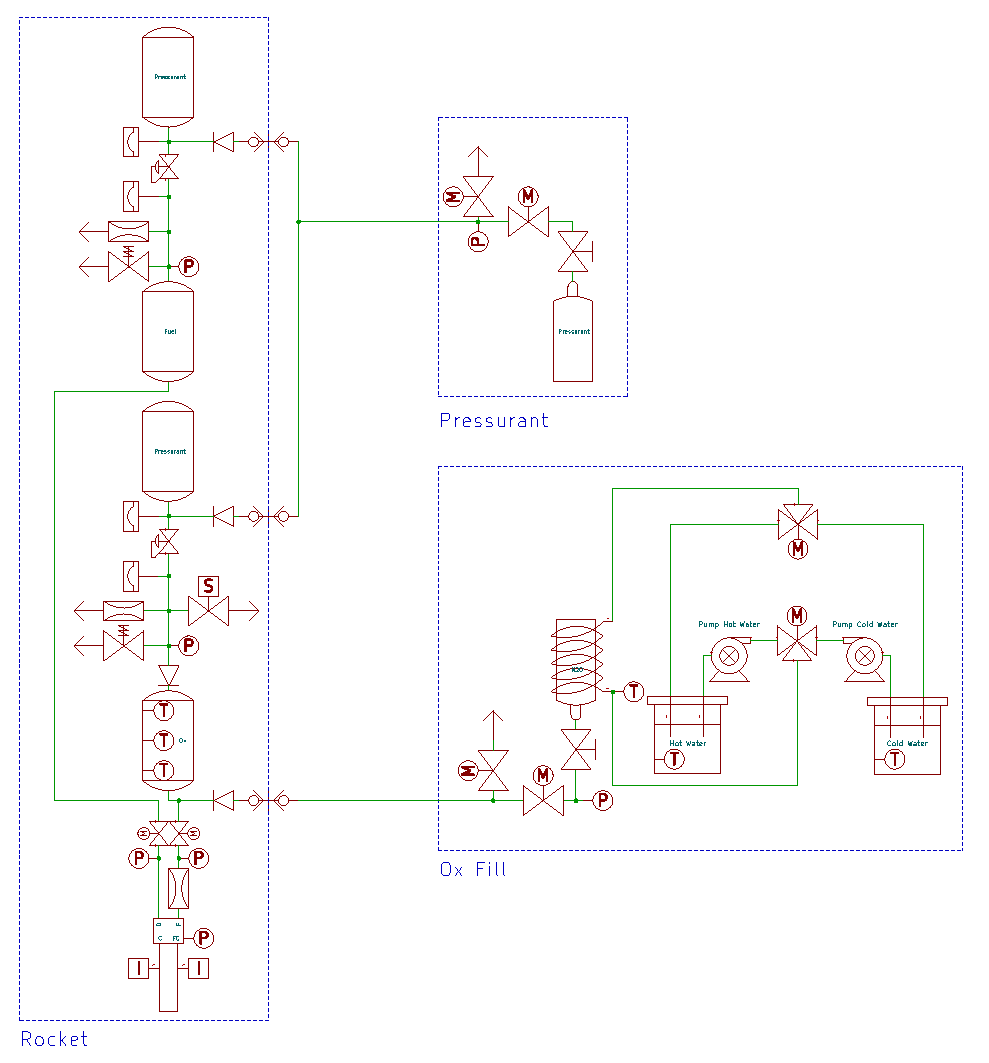
\includegraphics[width=0.9\textwidth]{SysArch/uHoubolt_complete_PnID.pdf}
    \caption{\uH Piping and Instrumentation Diagram (PnID)}
    \label{fig:full_pnid}
\end{figure}

Visible here is the PnID for the complete fluid system. This includes the rocket itself, as well as the Ground Support Equipment which encompasses the Pressurant and Ox Fill System. The three connections between the rocket and the GSE are quick connect fittings which are connected to a movable arm  to automatically disconnect them shortly before launch. See \cref{sec:gndsys} for more info on the GSE and \cref{sec:umbilicals} for the umbilicals specifically.

\subsection{Mass Budget}
\Cref{tab:massbudget} show the current mass budget for \uH.

\begin{table}[]
\centering
\begin{tabular}{|l|l|}
\hline
\textbf{Component} & \multicolumn{1}{c|}{\textbf{Mass in g}} \\ \hline
Airframe & 1900 \\ \hline
Recovery & 800 \\ \hline
Avionics & 400 \\ \hline
Payload & 1000 \\ \hline
Oxidizer System & 2600 \\ \hline
Fuel System & 1600 \\ \hline
Engine Section & 650 \\ \hline
\textbf{Total Mass Dry} & \textbf{8950} \\ \hline
Oxidizer & 2100 \\ \hline
Fuel & 700 \\ \hline
Pressurant & 290 \\ \hline
\textbf{Total Mass Wet} & \textbf{12040} \\ \hline
\end{tabular}
\caption{General System Data}
\label{tab:massbudget}
\end{table}

\subsection{Flight Simulation}

A flight simulation was performed with OpenRocket \cite{openrocket}, using a model of the vehicle closely matched to the CAD model and mass budget. The OpenRocket engine configuration (representing the whole propulsion system) was generated using ORLEG \cite{orleg}, which, in addition to changes in mass, also incorporates changes of the center of gravity location due to emptying propellant tanks and flowing pressurant gas as well as the effect of the changing ambient pressure on the engine performance. Assuming medium wind speeds and a launch downwind, the simulation yields the following results:

\begin{itemize}
\item Apogee: \SI{3558}{\meter}
\item Maximum velocity: \SI{302}{\meter\per\second} (Mach 0.91)
\item Maximum acceleration: \SI{51.5}{\meter\per\second\squared}
\item Flight time to apogee: \SI{27.8}{\second}
\item Total flight time: \SI{217}{\second}
\end{itemize}

Assuming an effective launch rail length of \SI{6}{\meter} (total length of \SI{7}{\meter} minus the distance between the rail buttons of about \SI{1}{\meter}) the vehicle has a velocity of \SI{22.2}{\meter\per\second} when leaving the rail and is aerodynamically stable.



\newpage

\section{Propulsion} \label{sec:prop}

Thrust is provided by a SRAD pressure fed bi-propellant liquid propulsion system. It utilizes nitrous oxide and ethanol as propellants and is pressurized by two nitrogen tanks through mechanical pressure regulators. The system is optimized for simplicity, low mass and small size. It can roughly be divided into three main subsystems which are described in detail below: the propellant tanks with piping, the pressurization systems and the engine with its valves and fill connections. A diagram of the whole fluid system, including the connected ground systems, can be found in \Cref{sec:sysarch_fluidSystem}.

The entire propulsion system, which is shown in \Cref{fig:sysarch_prop_propSystem} is assembled separately from the rest of the vehicle and can be tested standalone without it. It is installed into the airframe by sliding it into the body tube from the rear as one integrated component, only requiring two electrical connectors to be plugged in and a few screws to be installed.

\begin{figure}[H]
\centering
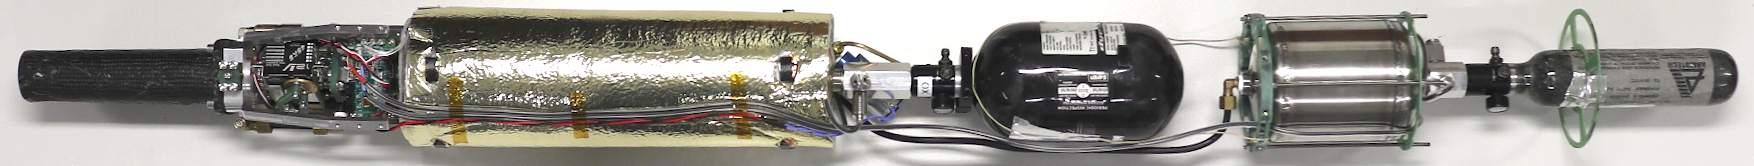
\includegraphics[width=\textwidth]{Propulsion/propSystem.png}
\caption{Complete propulsion system, ready to be installed into the airframe}
\label{fig:sysarch_prop_propSystem}
\end{figure}

\subsection{General Parameters}

The thrust is chosen to be \SI{600}{\newton} at liftoff as a trade-off between sufficient launch acceleration for aerodynamic stability and the capacity of the engine testing infrastructure. The chamber pressure and oxidizer/fuel mass flow ratio (O/F ratio) is chosen as a trade off between engine efficiency, combustion temperature, propellant mass flows and feed pressures.
As a compromise between high efficiency, low heat transfer into the thrust chamber and low feed pressures, a chamber pressure of \SI{15}{\bar} is chosen. \Cref{fig:sysarch_engPerf} shows various engine parameters as a function of the O/F ratio.

\begin{figure}[H]
\centering
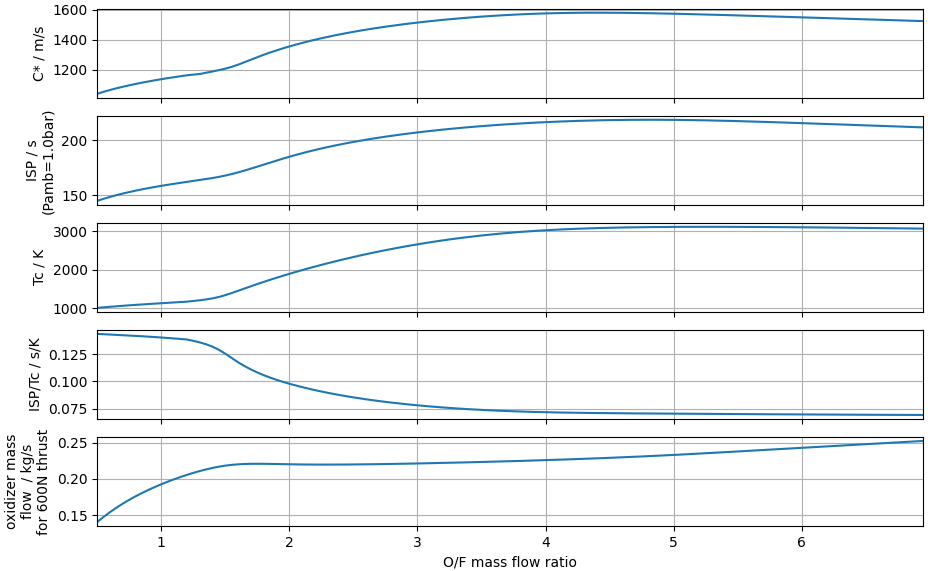
\includegraphics[width=\textwidth]{Propulsion/engineParameters.png}
\caption{Ideal engine performance parameters as a function of the oxidizer/fuel mass flow ratio at a chamber pressure of \SI{15}{\bar}}
\label{fig:sysarch_engPerf}
\end{figure}

Since the oxidizer mass flow rate is nearly constant at ratios above 1.5 and smaller ratios lead to unacceptable efficiency, this metric can be ignored. The fuel mass flow rate is not plotted but favors high ratios. The efficiency to combustion temperature ratio is highest at low O/F ratios but the efficiency is estimated to impact the vehicle mass more than the combustion temperature so a higher mass flow ratio of 3.0 is chosen based on this data.

As the vehicle will not reach high altitudes, the expansion ratio is sized for an ambient air pressure of \SI{1000}{\milli\bar}.
When assuming a \SI{93}{\percent} C* and ISP efficiency (based on previous engine testing data) and a thrust of \SI{600}{\newton}, the following engine parameters were calculated using the self developed Python program ORLEG \cite{orleg} which uses the CEA \cite{CEA} Python wrapper RocketCEA \cite{RocketCEA}:

\begin{itemize}
\item throat diameter: \SI{19}{\milli\meter}
\item nozzle exit diameter: \SI{32}{\milli\meter}
\item nozzle expansion ratio: 2.7
\item combustion temperature: \SI{2632}{\kelvin}
\item c*: \SI{1405}{\meter\per\second}
\item ISP: \SI{192}{\second}
\item total mass flow rate: \SI{318}{\gram\per\second}
\item fuel mass flow rate: \SI{79}{\gram\per\second}
\item oxidizer mass flow rate: \SI{238}{\gram\per\second}
\end{itemize}

Considering the complete vehicle design, a burn time of about \SI{8}{\second} is necessary to reach the intended target altitude of \SI{3}{\kilo\meter}. The fuel tank is sized to a volume of \SI{900}{\milli\liter} and the oxidizer tank to \SI{2400}{\milli\liter}, fitting about \SI{700}{\gram} of fuel at ambient temperature and \SI{2085}{\gram} of oxidizer at a temperature of \SI{0}{\celsius} (see \cref{sec:sysarch_prop_oxLoad}) and an assumed fill level of 95\% due to boil-off between filling and launch. This gives a maximum burn time of up to \SI{8.8}{\second}, when a constant thrust of \SI{600}{\newton} is assumed. As the tank pressures and therefore mass flow rates and thrust drop off during the burn due to non-ideal pressure regulators, the burn time increases slightly.

\subsection{Propellant Tanks and Piping}

\begin{figure}[H]
\centering
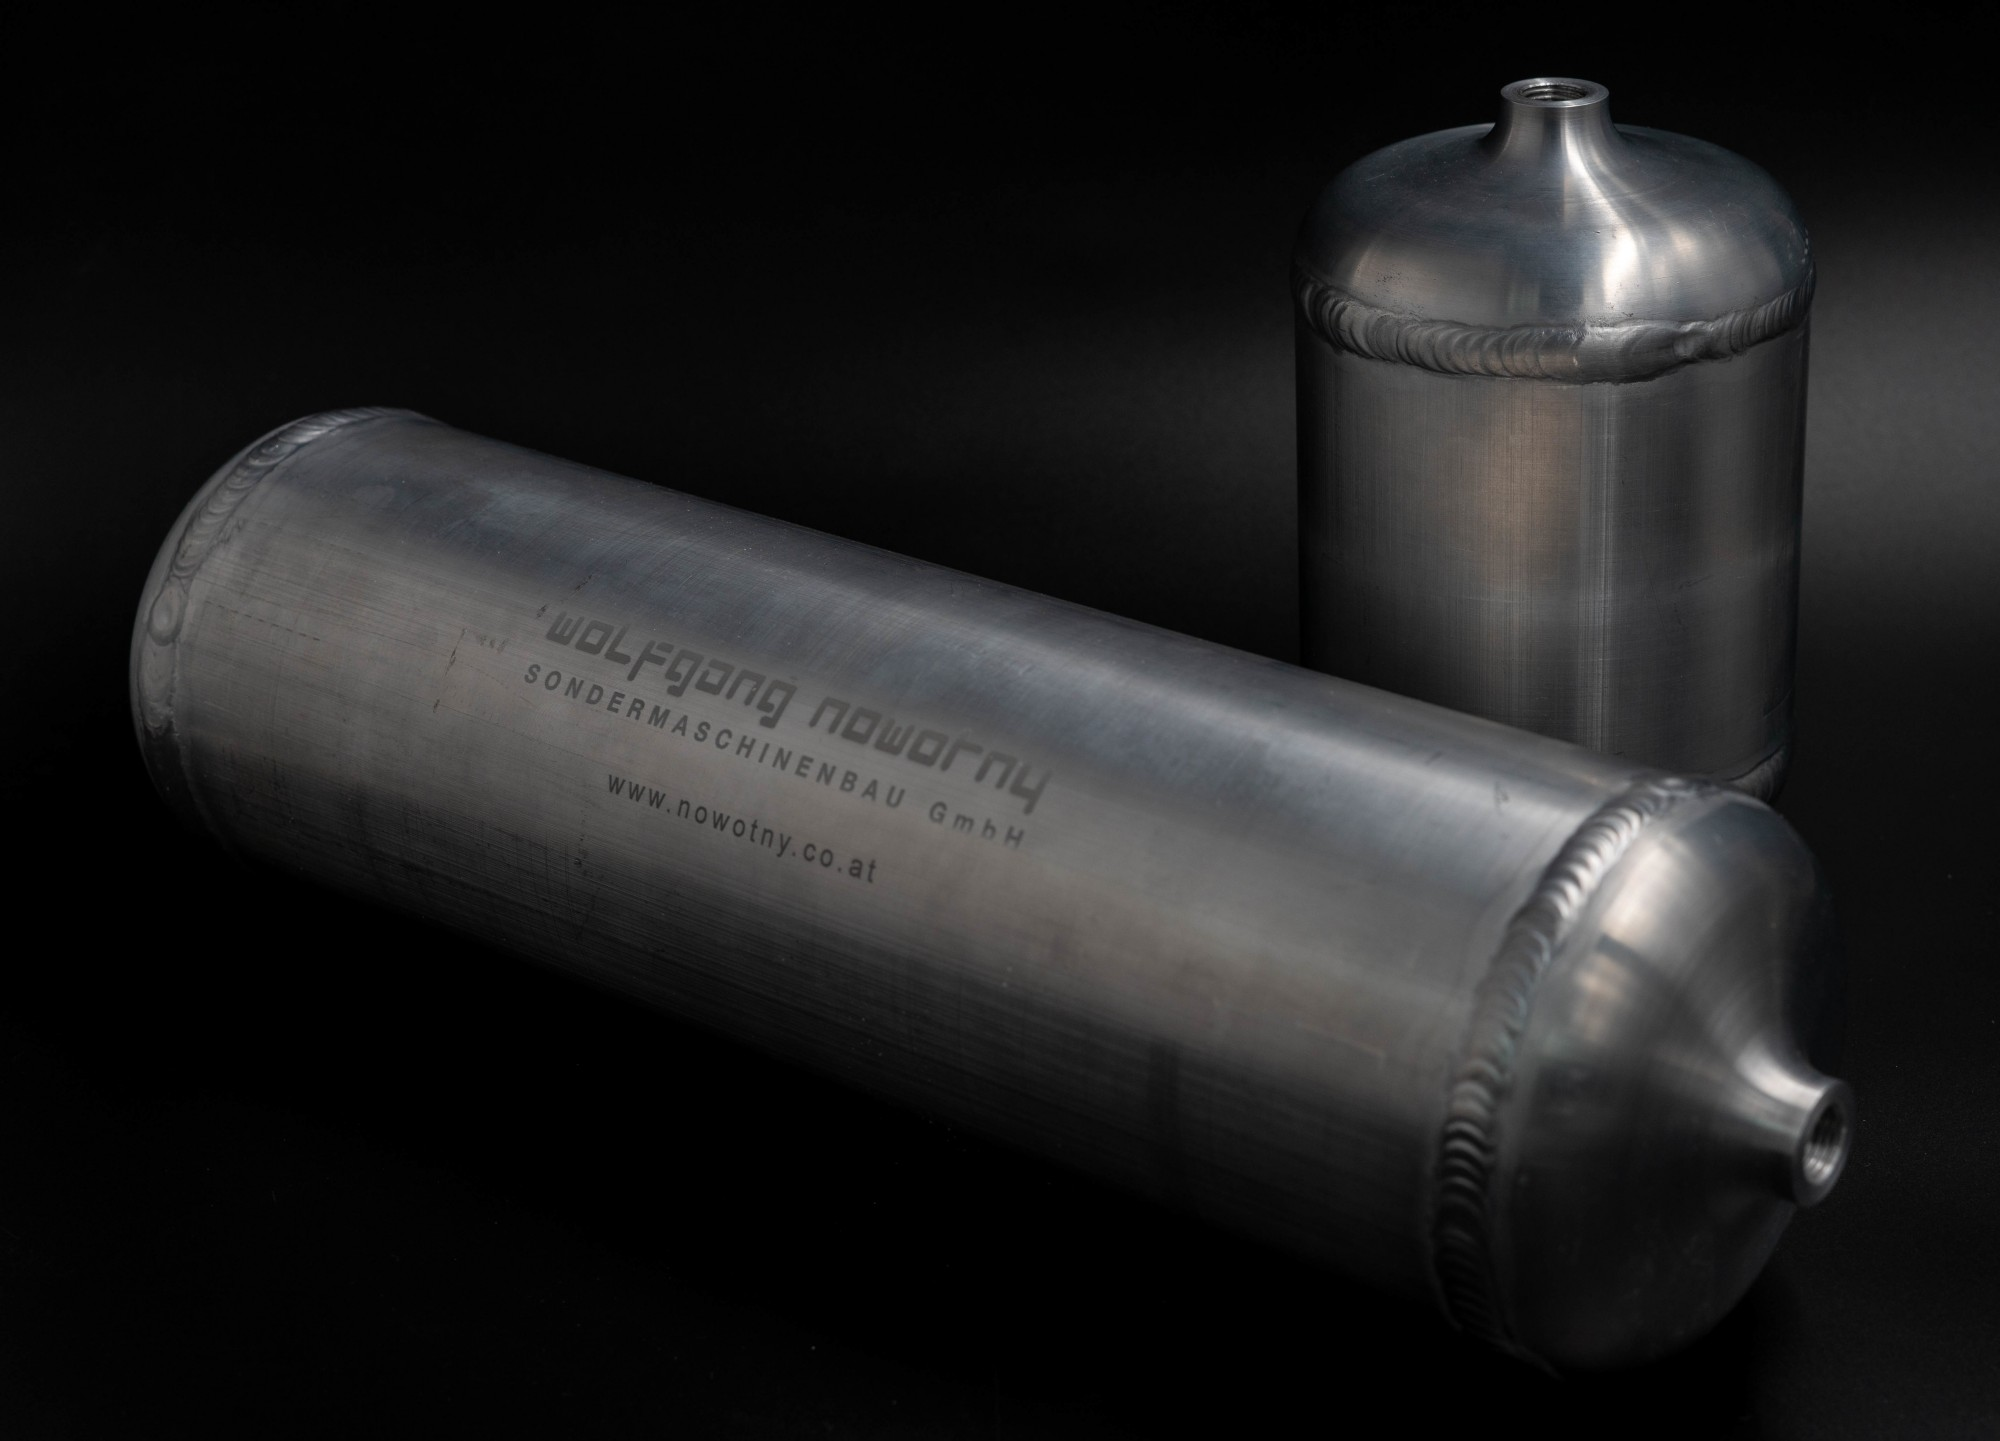
\includegraphics[width=\textwidth]{Propulsion/propTanks.jpg}
\caption{Aluminium propellant tanks}
\label{fig:sysarch_prop_propTanks}
\end{figure}

The propellant tanks, shown in \Cref{fig:sysarch_prop_propTanks} are manufactured from aluminium in three parts each that are welded together, the two end-caps with threaded connections and a tube in between. They were designed by the team but are one of the few components manufactured externally. This allowed for a more optimized end-cap design to be manufactured and additionally the welds were done by a professional welder, assuring consistency.

Sharing the end-cap design, the fuel and oxidizer tanks have a diameter of \SI{101}{\milli\meter}. A length of \SI{192}{\milli\meter} for fuel and \SI{387}{\milli\meter} for oxidizer gives the tanks a volume of \SI{900}{\milli\liter} and  \SI{2400}{\milli\liter} and a mass of \SI{594}{\gram} and \SI{1170}{\gram}.

To minimize mass, a heat treated high strength aluminium alloy is used, which at the same time has to be weldable. The choice fell on EN AW-6082. As there were uncertainties regarding the strength of the welded joints, which is crucial for this application, representative samples of the material were cut in half and welded back together by the designated tank manufacturer using the process planned for the tanks. After heat treatment for hardening, the samples were professionally tested for tensile strength, yielding good results. Based on those, the tanks were designed for a burst pressure of \SI{125}{\bar} and manufactured before receiving the same heat treatment as the samples.

The maximum nominal operating pressure of the tanks is about \SI{50}{\bar} for oxidizer and \SI{40}{\bar} for fuel. As under some circumstances, the tanks could be exposed to up to the \SI{60}{\bar} set pressure of the safety valves, the pressure used for proof testing was based on this value. With a 50\% safety factor, the tanks were hydrostatically tested at \SI{90}{\bar} for an extended amount of time, without showing leaks or other abnormalities. The detailed test report can be found in \Cref{sec:app_proof_pressure_testing}.

The oxidizer tank is axially supported by its connection to the engine assembly via the oxidizer tube and in turn axially supports the oxidizer pressurant system. Radial support against the body tube is provided by 3D-printed plastic spacers. As the pressurant fill connection needs to be aligned with the other fill connections, the connection between the oxidizer tube and the oxidizer valve (which is rigidly mounted to the engine) can be mounted with arbitrary rotation, as described in \Cref{sec:sysarch_prop_mainvalves}. To reduce heat flow into the tank, which causes the liquid oxidizer to boil off, the tank is wrapped in thermal insulation.

\begin{figure}[H]
\centering
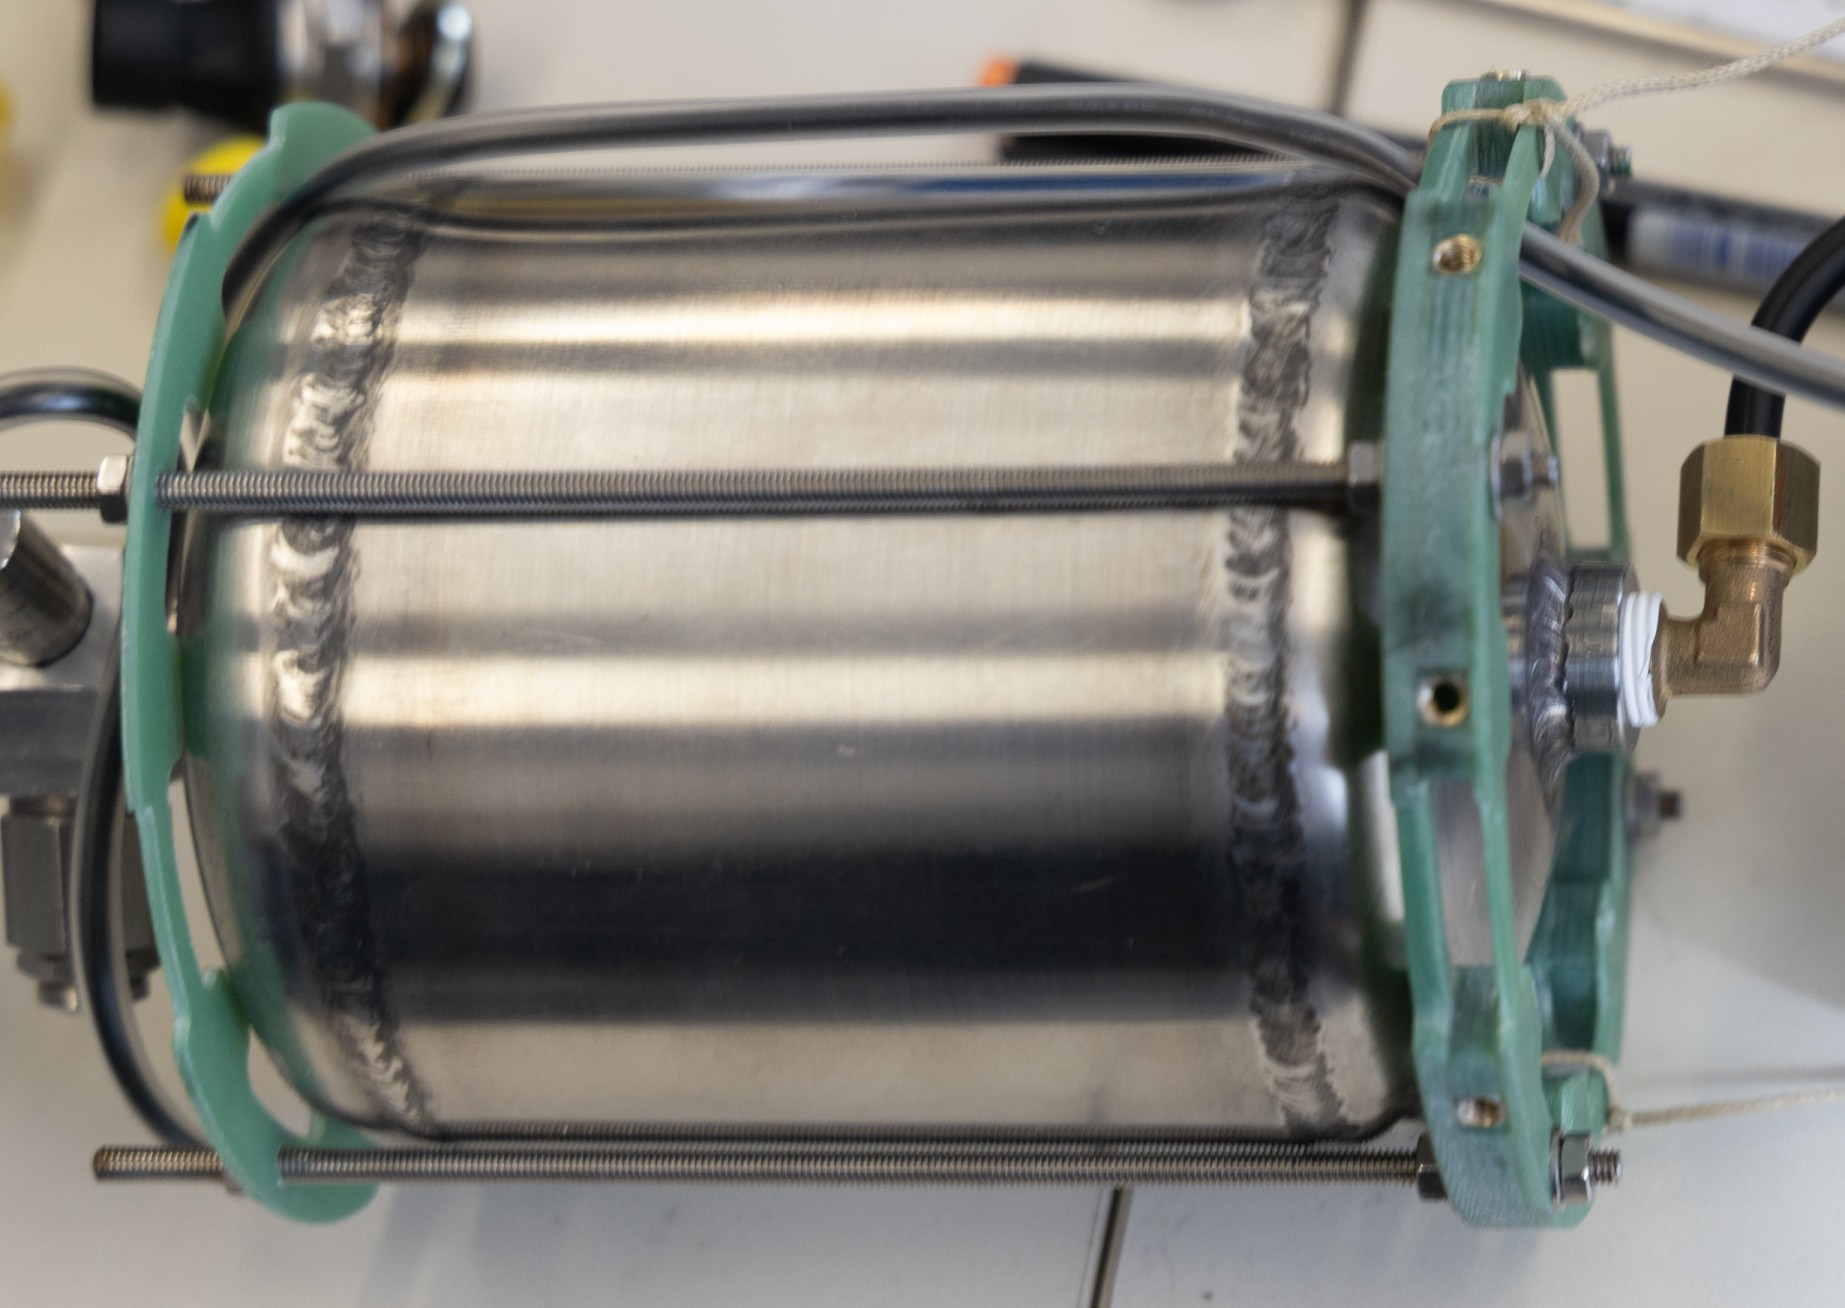
\includegraphics[width=0.7\textwidth]{Propulsion/fuelTankMounting.jpg}
\caption{Steel Prototype Fuel Tank in its mounting cage}
\label{fig:sysarch_prop_fuelTankMounting}
\end{figure}

The fuel tank also supports the fuel pressurization system but it is not rigidly connected to the rest of the propulsion system. Instead, the fuel tank is clamped in a cage made of GFRP plates and threaded rods (shown in \Cref{fig:sysarch_prop_fuelTankMounting}), which in turn is attached to the body tube via radial screws. During installation of the propulsion system into the body tube from the rear, the fuel system is pushed in by the rest of the propulsion system. It can then be manipulated from the front to seat the radial screws. As the fuel tank can be rotated within its mounting cage with a bit of force, the fuel systems rotation can then be finely adjusted to align the pressurant fill connection with the associated opening in the body tube. While the process may sound tedious, it is actually pretty simple and quick. To avoid the fuel system getting pulled out by the flexible fuel tube connecting it to the engine when pulling out the propulsion system, a piece of string connects the two subsystems and removes any tension from the fuel tube.

The connection between the fuel tank and engine is made with an aluminium-poliamide composite tube with an outside diameter of \SI{6}{\milli\meter} and a wall thickness of \SI{1}{\milli\meter}. It is flexible, light weight and compatible with standard compression ring fittings, making it well suited for this application. While the pressure rating given by the manufacturer is not sufficient for the application, it is given with a higher than needed safety factor, and the tube was successfully pressure tested to twice its maximum operating pressure.

\subsection{Pressurization System}

The fuel and oxidizer tanks are pressurized by nitrogen from two COPVs via mechanical pressure regulators. The COPVs with max. pressure of \SI{300}{\bar} and volumes of \SI{800}{\milli\liter} and \SI{250}{\milli\liter} for the fuel and oxidizer systems as well as the pressure regulators are COTS components, originally intended for pressurizing Paintball equipment.

The regulators exhibit less than ideal performance, with the fuel pressure dropping from \SI{40}{\bar} static pressure to \SI{30}{\bar} at startup due to the mass flow demand and then progressively down to \SI{25}{\bar} during the burn due to decreasing pressurant tank pressure. The oxidizer regulator behaves similarly with a pressure drop from \SI{50}{\bar} static to \SI{40}{\bar} at startup and down to \SI{35}{\bar} during the burn.
While this behaviour is far from ideal and additionally varies a bit from run to run, it is good enough for this vehicle.
The additional influence of the acceleration on the pressure differential between the top of the propellant tanks and the injector can be ignored due to the vehicles small size.

Active pressure control using electrically actuated valves and a software control loop was evaluated with good preliminary results but got abandoned in favor of the simple solution using mechanical regulators. For larger vehicles or more stringent pressure accuracy requirements, active control would be the preferred method though.

No pressurization valves are used, so the propellant tanks get pressurized as soon as the pressurant tanks get filled (the regulators include fill connections and check valves), which (apart from a partial pre-pressurization before oxidizer filling) only happens shortly before liftoff, see \Cref{sec:prop_pressfill}.

\begin{figure}[H]
\centering
\subfloat[Fuel]{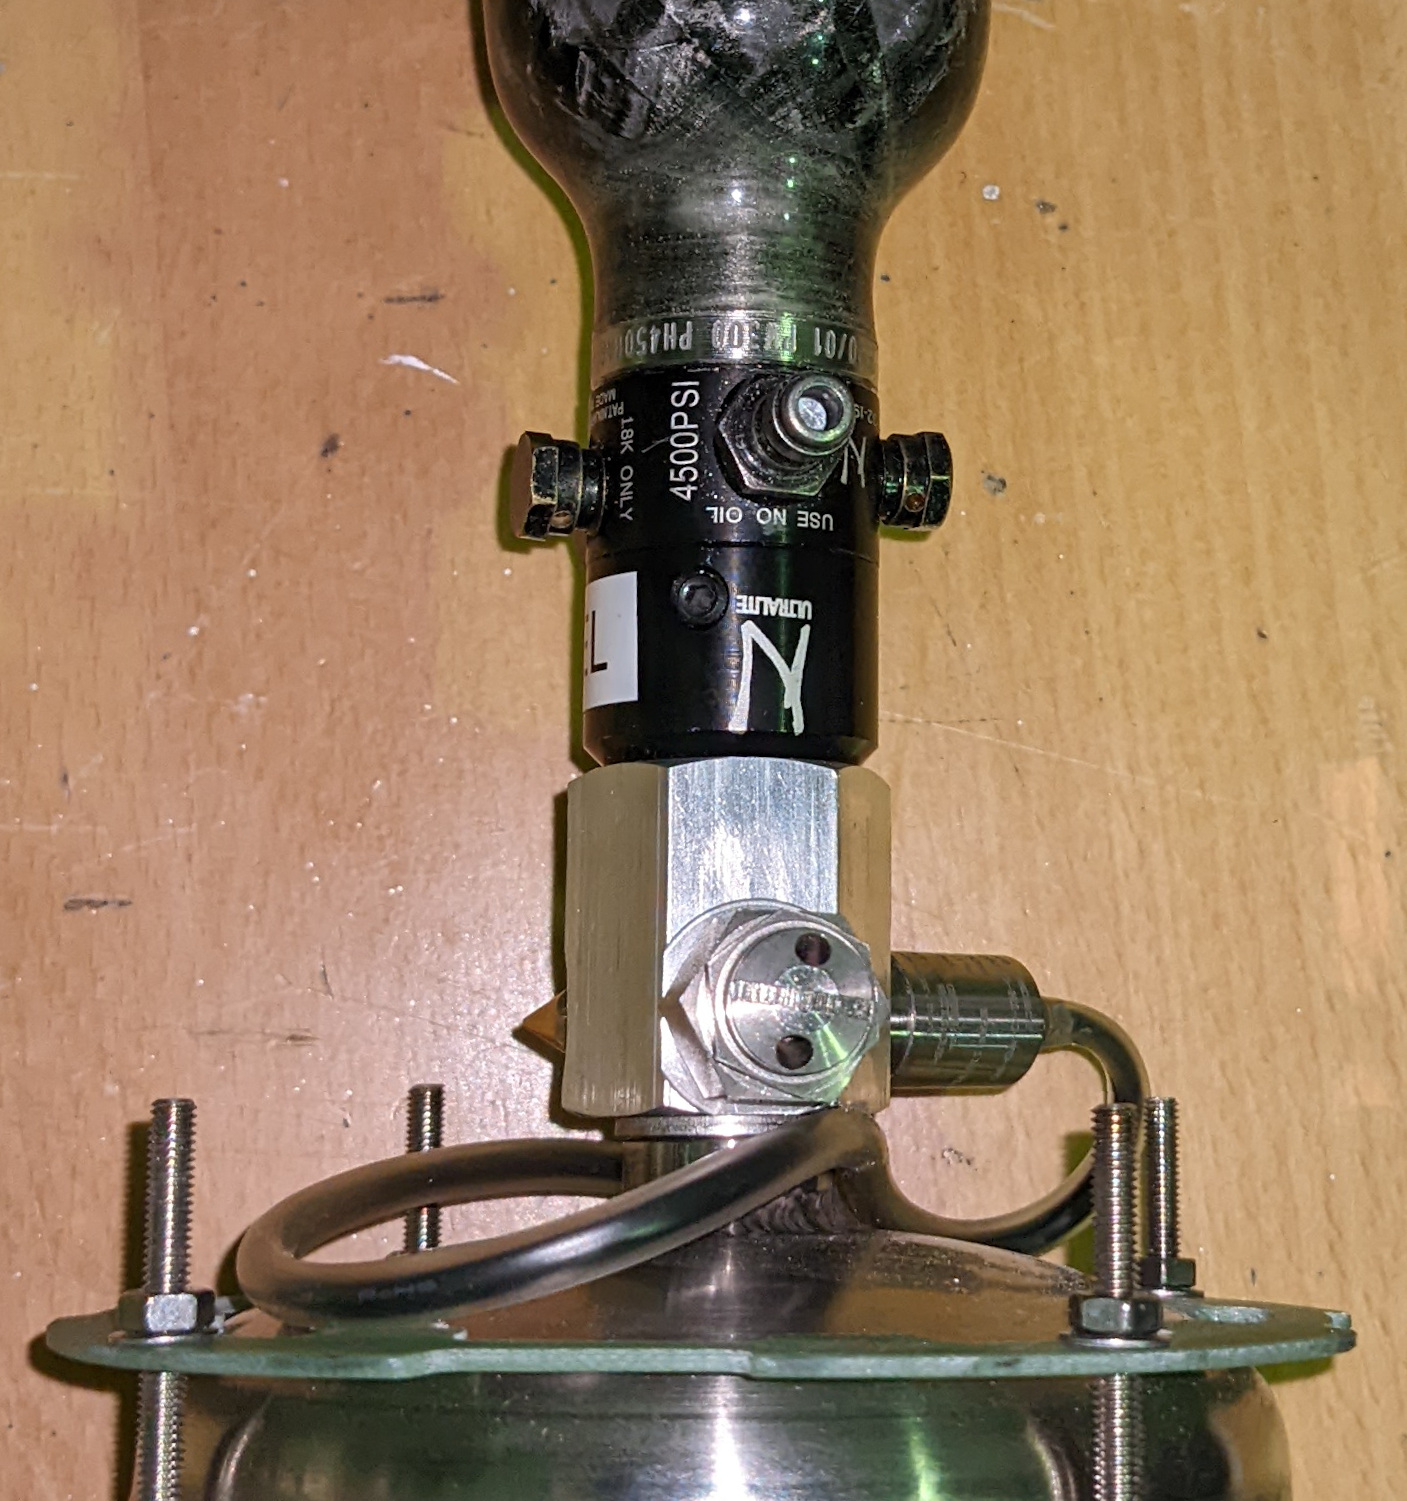
\includegraphics[width=0.3\textwidth]{Propulsion/fuelManifold.jpg}}
\subfloat[Oxidizer]{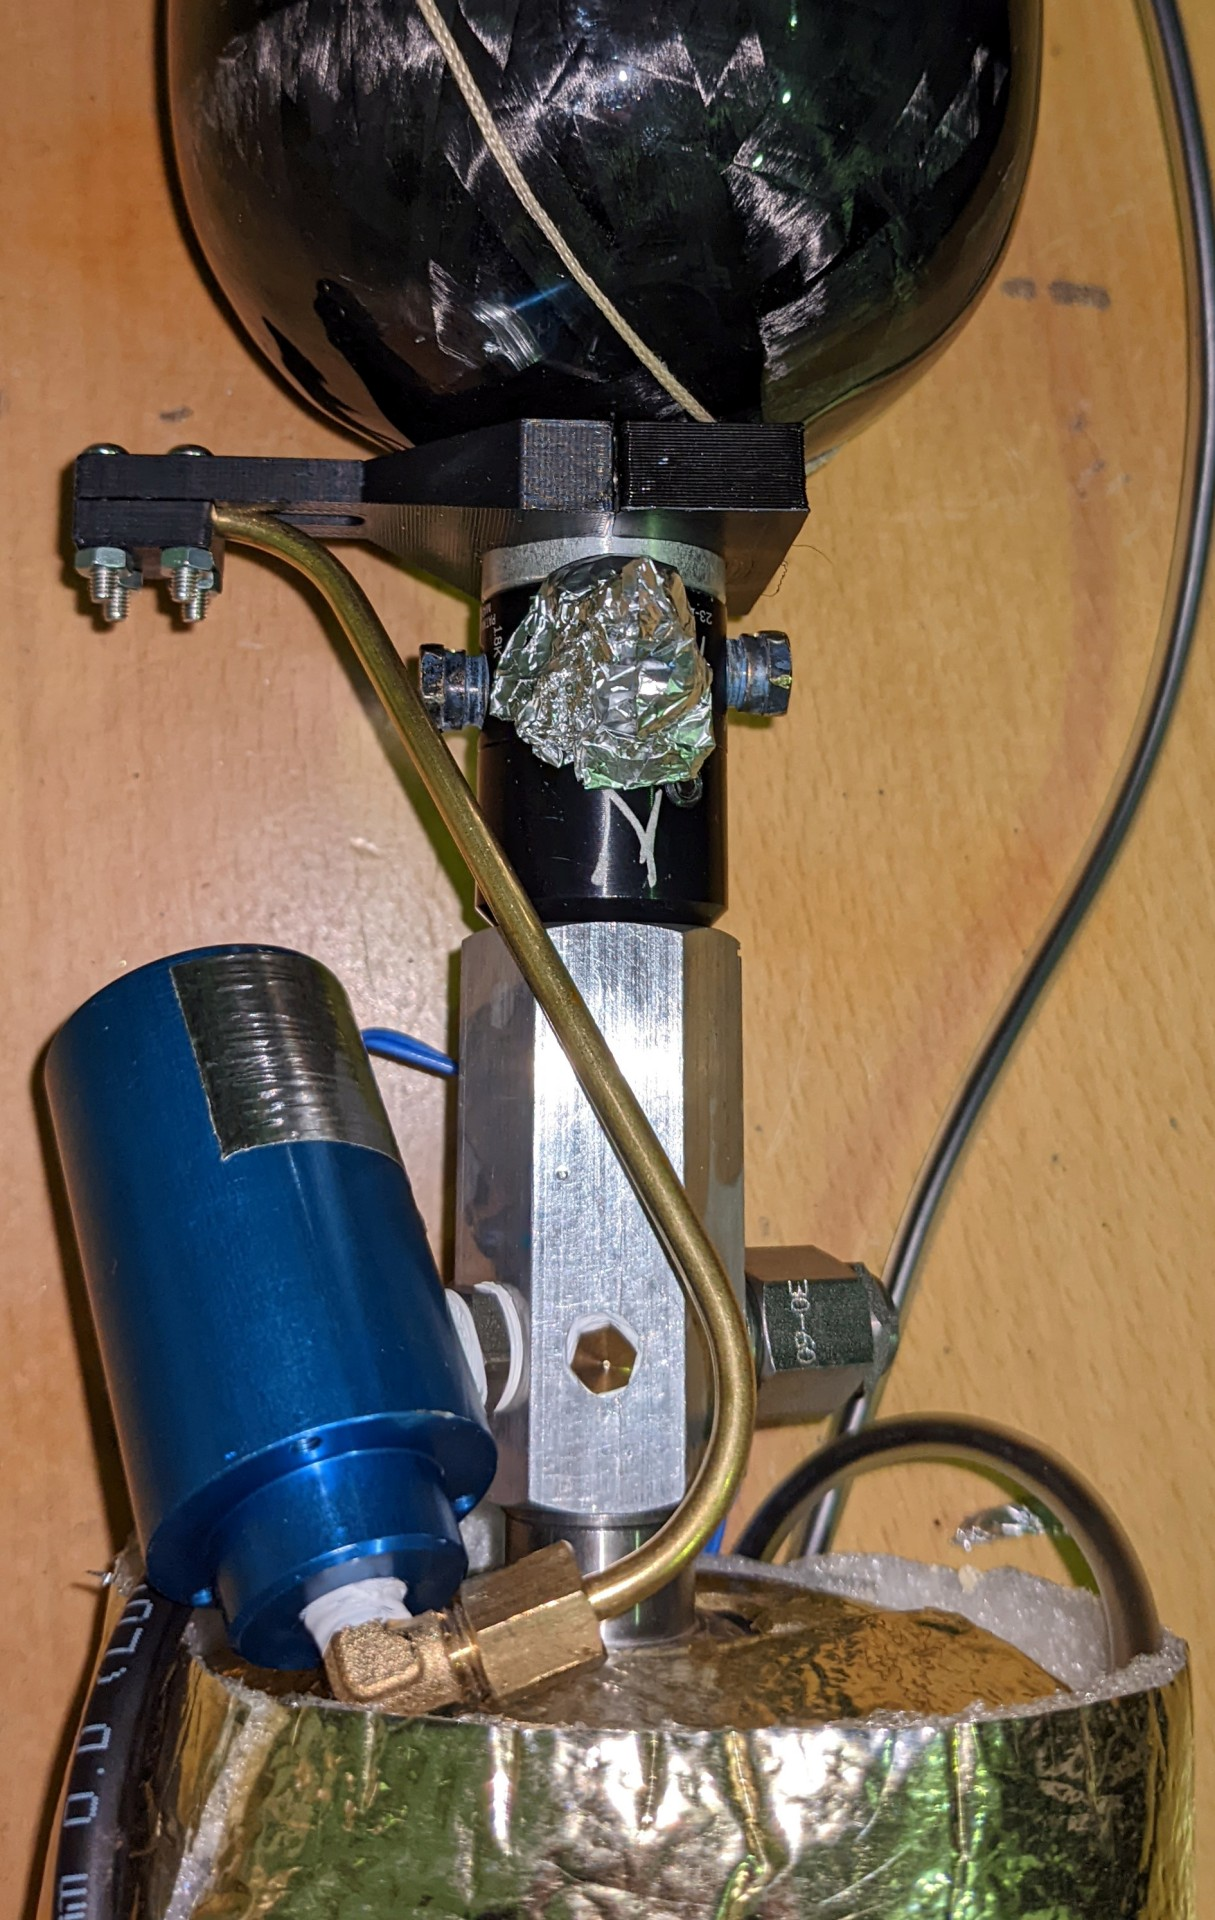
\includegraphics[width=0.3\textwidth]{Propulsion/oxManifold.jpg}}
\subfloat[Oxidizer]{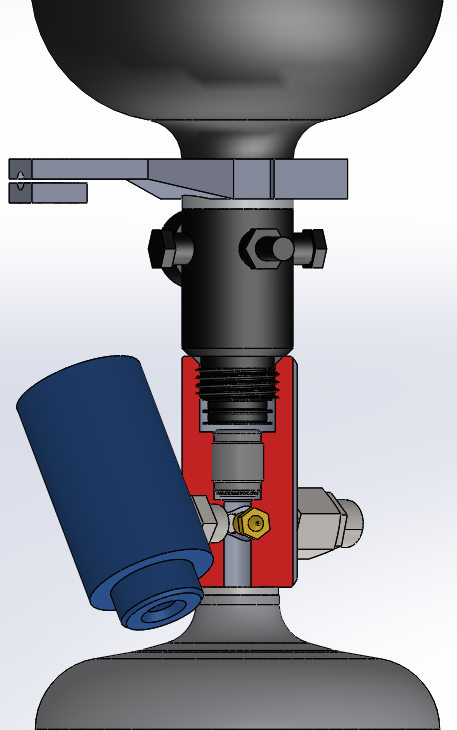
\includegraphics[width=0.3\textwidth]{Propulsion/oxManifoldCut.png}}
\caption{Pressurization manifolds with connected components}
\label{fig:sysarch_prop_pressManifolds}
\end{figure}

The output sides of the pressure regulators are screwed into the top of aluminium manifolds, which connects multiple components together. In case of the oxidizer, an inline check valve is integrated inside the manifold after the regulator to prevent any oxidizer flowing back into the pressurization system, this is not needed for the fuel side. The bottom side of the manifolds is screwed into the top of the propellant tanks. Connected on the sides of each manifold are a tank pressure sensor, a safety valve and a bleed orifice. The assemblies are shown in \cref{fig:sysarch_prop_pressManifolds}.

The safety valves are set to their maximum of \SI{60}{\bar}, well under the tanks proof and burst pressures. The bleed orifice consists of a \SI{0.1}{\milli\meter} 3D-printing nozzle that is used to slowly depressurize the system over time. This helps to safe the vehicle in case of a complete avionics failure and does not negatively impact normal operations. 

On the oxidizer manifold, a solenoid vent valve is installed as well, to allow for active regulation of the tank pressure and thus oxidizer temperature during and after filling, see \Cref{sec:sysarch_prop_oxLoad}. The output of the solenoid valve flows through a tube to an opening in the body tube, to not cause pressure spikes within the airframe that could trigger the recovery electronics, and to make the vented plume visible, which helps recognize the completion of the filling process.

The regulators include two burst discs, one with a \SI{517}{\bar} burst pressure to protect the pressurant bottle and one with a \SI{124}{\bar} burst pressure on the output. Since this output burst disc's burst pressure is much greater than the opening pressure of the safety valves, this burst disc is not expected to be needed unless the safety valves fail and an overpressure event is caused. In case of the oxidizer system, the burst disc can only protect against overpressure caused by a regulator failure, as overpressure originating from the oxidizer tank can't flow back to the burst disc through the check valve.

Both pressurization system assemblies are axially supported by the connection to their respective propellant tank. Radial support against the body tube for the pressurant tanks is provided by a GFRP spacer plate for the fuel tank and 3D-printed plastic spacers for the oxidizer tank.

\subsection{Engine, Valves and Fill Connections}
\label{sec:engine_valves_fill_connections}

\begin{figure}[H]
\centering
\subfloat{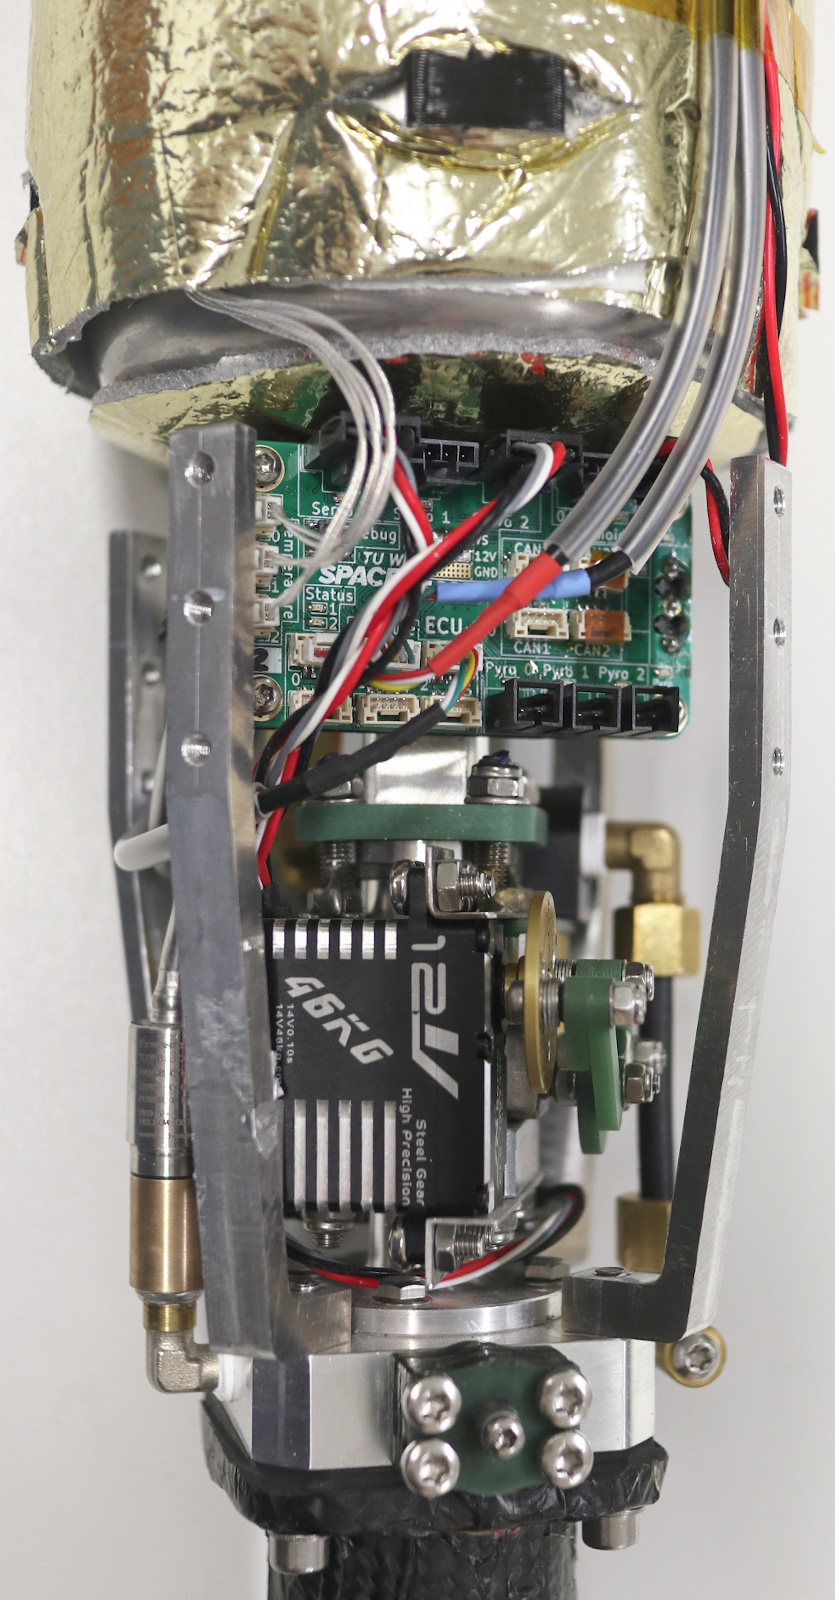
\includegraphics[width=0.25\textwidth]{Propulsion/engineAssy_1.jpg}}
\subfloat{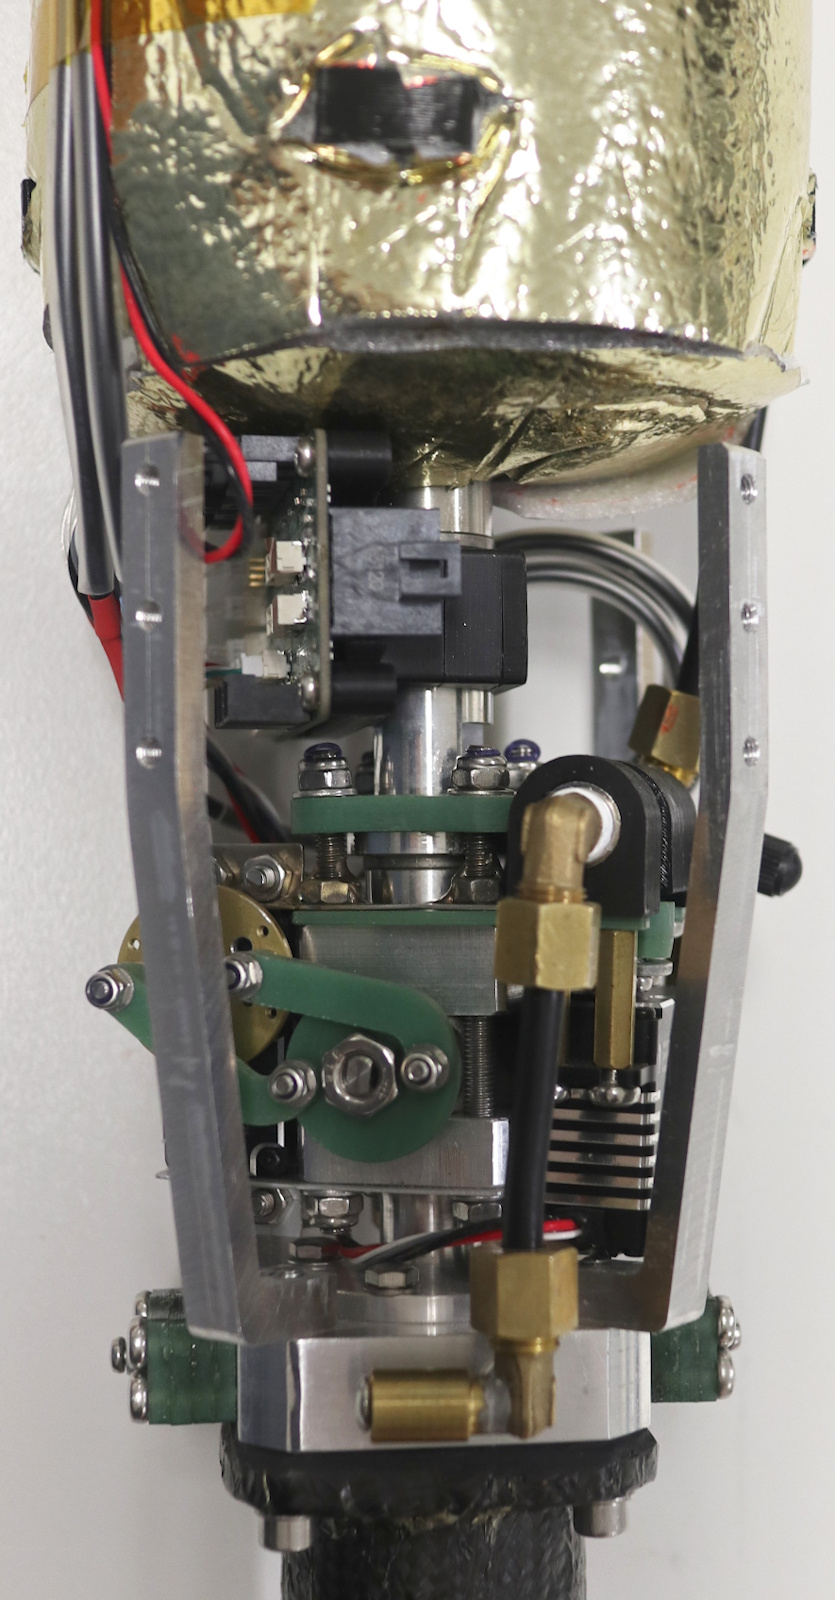
\includegraphics[width=0.25\textwidth]{Propulsion/engineAssy_2.jpg}}
\subfloat{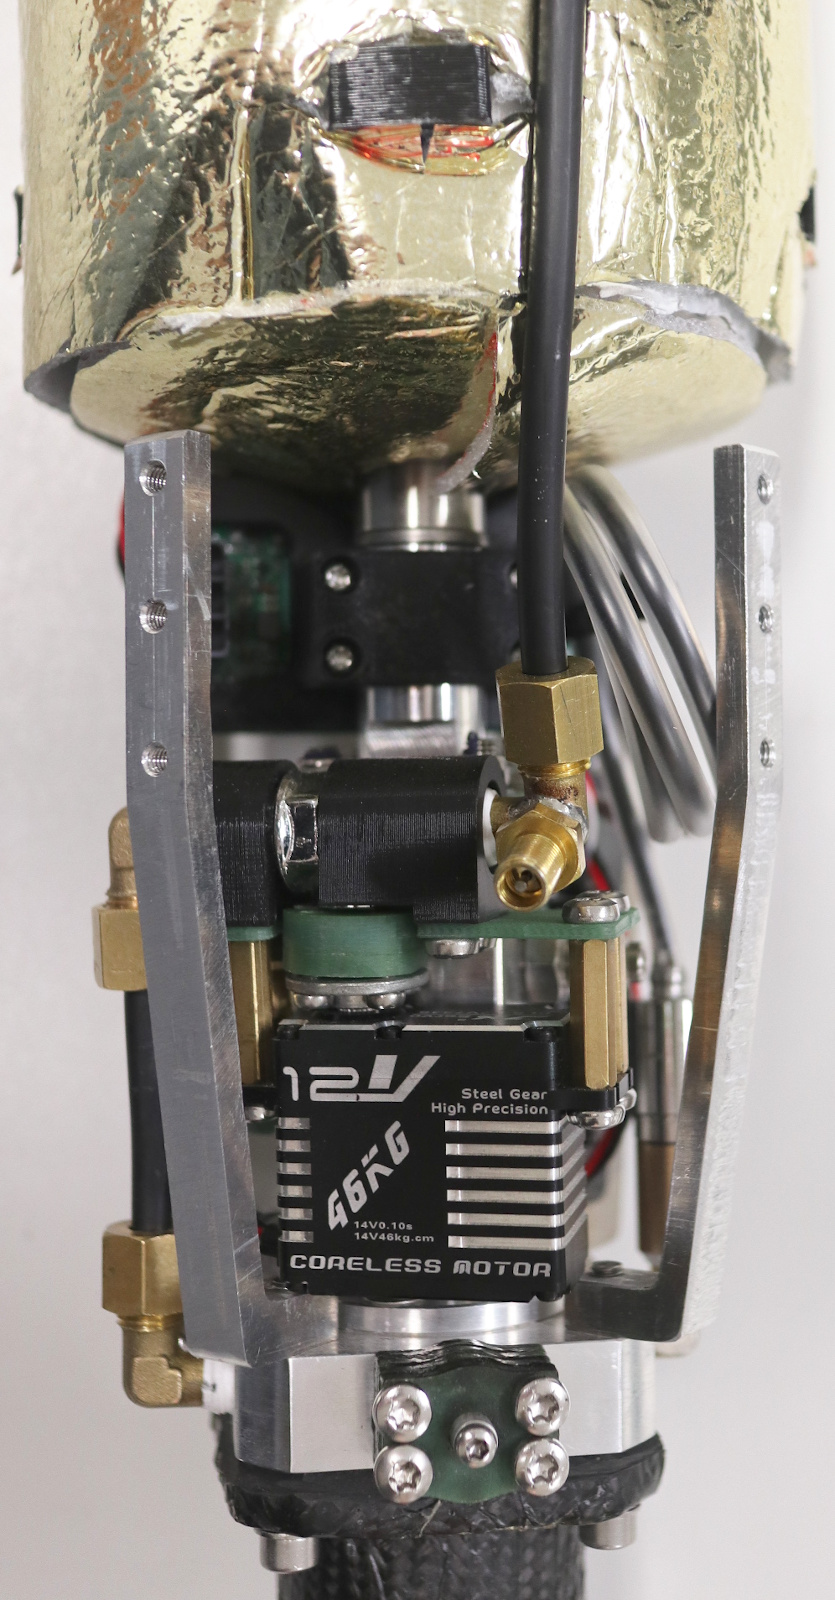
\includegraphics[width=0.25\textwidth]{Propulsion/engineAssy_3.jpg}}
\subfloat{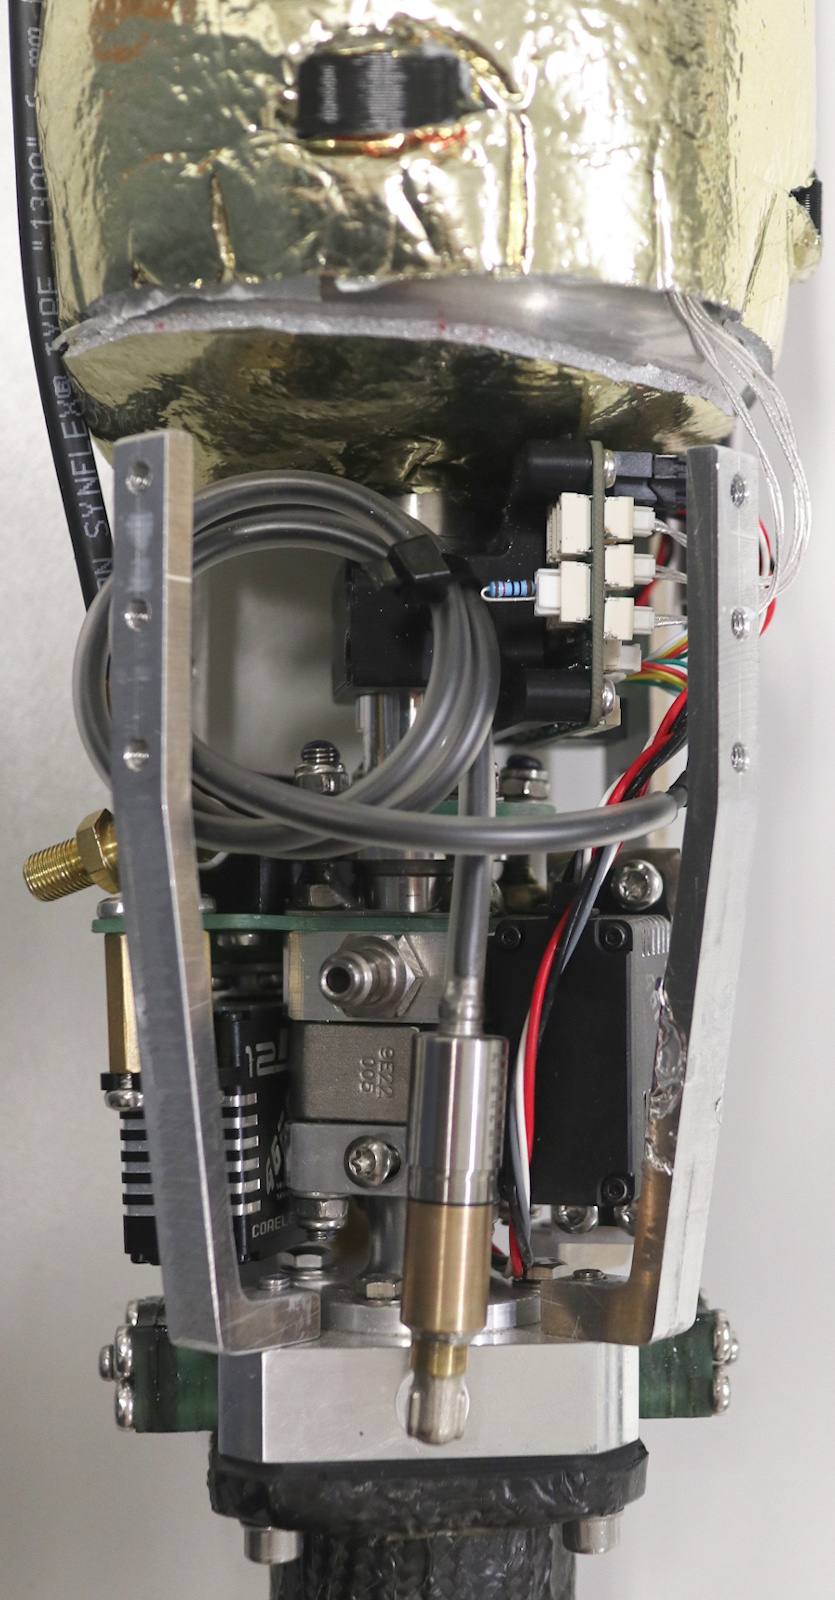
\includegraphics[width=0.25\textwidth]{Propulsion/engineAssy_4.jpg}}
\caption{Engine assembly, shown from multiple sides}
\label{fig:sysarch_prop_engineAssy}
\end{figure}

The engine assembly, shown in \Cref{fig:sysarch_prop_engineAssy}, consists of the engine with injector and thrust chamber, the  main propellant valves with actuators, a redundant integrated ignition system, propellant fill connections, pressure sensors, propulsion avionics and structural components. The assembly features a high integration density and low mass, which is achieved mainly by the use of a semi-custom oxidizer valve, custom manifold components and fill connections with integrated check valves. The avionics are described in detail in \Cref{sec:avi}, the other components in this section.

The central component of the assembly is the aluminium engine head. It sits atop the thrust chamber (\Cref{sec:prop_thrustchamber}) and is mounted to the airframe (\Cref{sec:aerostructure_lowercoupler}) via four aluminium struts that transfer most of the thrust force during powered ascent and carry the engine and oxidizer assemblies during descent. On the four sides of the engine head, the ignition system (\Cref{sec:prop_ignition}) is integrated, as are the fuel connection, a venturi for fuel flow regulation (\Cref{sec:prop_injector}) and a chamber pressure sensor connection via an elbow adapter.

Mounted to the top of the engine head is the injector (\Cref{sec:prop_injector}). Together they form an internal annular volume which is used for distributing fuel to the fuel injection orifices. The injector doubles as a part of the main oxidizer valve, whose other components are mounted on top. The propulsion avionics are mounted to the oxidizer tube above this valve, which doubles as a structural component. The main fuel valve and the actuators for both valves sit to the sides of the oxidizer valve assembly and are mounted to it.

\subsubsection{Main Valves and Fill Connections}\label{sec:sysarch_prop_mainvalves}

The main fuel valve is a small COTS ball valve, mounted to the side of the oxidizer valve.
An elbow fitting connects the valve to a short tube going down into the engine head. The associated fitting on the engine head also includes a connection to attach an injector pressure sensor. While the small sensors used in other parts of the system would fit here, this connection is only used for ground testing with larger sensors (that only fit with the Fincan removed), as the availability of the small type is limited and the measurement is not needed for flight.
Another elbow fitting connecting to the pipe going up to the fuel tank also has the fuel fill connection attached. It consists of a repurposed tyre fill connector with integrated check valve. While normally used for pressures below \SI{10}{\bar}, testing has shown it to still work reliably at pressures of \SI{60}{\bar} or higher. Connecting it close to the valve ensures that the tube leading up to the fuel tank is always filled with fuel and doesn't trap any air, assuring consistent engine startup behaviour.
The valve is actuated by a standard size high torque RC servo motor mounted co-axially.

The main oxidizer valve consists of the body and inner components of a COTS Swagelok 3-piece ball valve (with upstream vented ball) in combination with custom aluminium flanges.
The lower flange is part of the injector, avoiding an additional connections and setting the orientation of the valve assembly and all connections mounted to it while also saving space and mass. The component also includes a connection to attach a pressure sensor, which -- for the same reason described for the fuel side in the previous paragraph -- is currently only used for ground testing.
The upper flange includes the connection for filling the oxidizer tank, which uses a repurposed Paintball fill connector with included check valve. It is rated for up to \SI{300}{\bar} and is -- apart from the o-ring which was replaced by a FKM one -- made from materials compatible with nitrous oxide. Apart from making for a very compact assembly, this design also avoids any gas to be trapped between the fill port and valve during filling, which might introduce variability to the startup behaviour. A piece of fine stainless steel mesh is added inside the fill connector to act as a filter.
The main valve is actuated by a standard size high torque RC servo motor mounted to the side of the valve, with the servo axle and valve stem coupled via a pair of push/pull rods.

The four threaded rods holding together the oxidizer valve are welded to plates in pairs to lock their rotation, simplifying assembly. One of the plates is also used as a mounting point for the oxidizer valve servo. The rods extend up above the valve and are additionally used to connect the oxidizer tube to the upper flange, with a bonded seal in between. This arrangement allows adjustment of the rotation of the tube and the oxidizer tank and pressurization system connected to it. As all fluid connections above are threaded and sealed with bonded seals, this feature is needed to correctly set the direction of the oxidizer pressurant fill connection to be the same as the oxidizer fill connection.

As similarly light weight pressure regulators with adjustable fill port angle have become available, this feature can be removed when upgrading to one of these regulators. In that case, the extended rods are not needed anymore, which would allow for a simpler design. The upper flange and tube could be made as one part and the oxidizer valve could be held together by four bolts screwed from the top into threaded holes in the lower flange / injector. The oxidizer servo mount would consist of plates screwed to threads on the side of the flanges, and to the servo via threaded spacers. This modification was not made to the EuRoC 2022 design due to time constraints but is recommended for future builds. 

\subsubsection{Injector and Mass Flow Regulation}\label{sec:prop_injector}

The aluminium injector, shown in \Cref{fig:sysarch_injCut}, is a quadruple unlike-doublet impingement type, with four radial fuel jets impinging with four axial oxidizer jets. It is relatively simple to manufacture and has delivered good reliability and adequate performance in hot fire testing.

\begin{figure}[H]
\centering
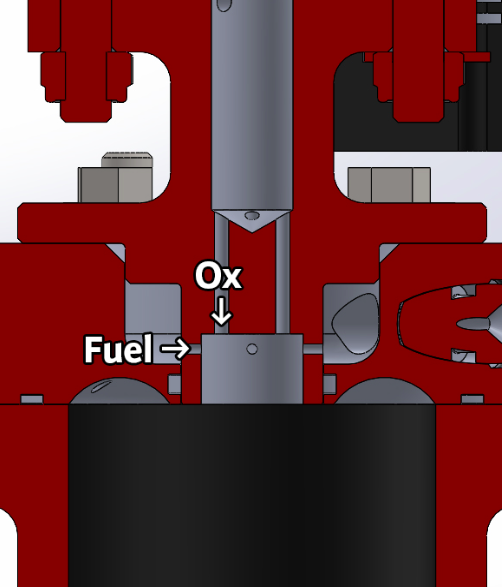
\includegraphics[width=0.5\textwidth]{Propulsion/injector_cut.png}
\caption{Cross section of the injector}
\label{fig:sysarch_injCut}
\end{figure}

The fuel mass flow is regulated by a cavitating venturi integrated into the engine head, which is shown in \Cref{fig:sysarch_prop_fuelVenturi}. Its throat diameter $A_t$ is \SI{1.4}{\milli\meter} and the experimentally determined discharge coefficient $C_d$ is 0.89. The mass flow through it for a given density $\rho$, vapor pressure $p_{sat}$ and inlet pressure $p$ is governed by the following equation, as long as the pressure drop is large enough to lead to cavitation at the throat:

\begin{equation}
\dot{m} = C_d * A_t * \sqrt{2 * \rho * (p - p_{sat})}
\end{equation}

The four fuel injector orifices with a diameter of \SI{1}{\milli\meter} are sized large enough to avoid cavitation and thus choking and small enough to cause a high injection velocity for good atomization and mixing.

\begin{figure}[H]
\centering
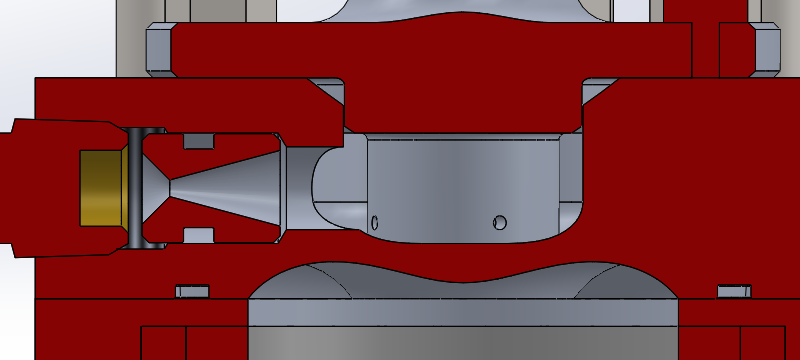
\includegraphics[width=0.8\textwidth]{Propulsion/fuelVenturi.png}
\caption{Engine cross section showing the fuel cavitating venturi. The brass fitting on the left is simplified.}
\label{fig:sysarch_prop_fuelVenturi}
\end{figure}

The liquid oxidizer with its vapor pressure significantly higher than the chamber pressure does not require a separate flow regulation device. Instead, it flashes to steam in the four injection orifices, which have a diameter of \SI{1.6}{\milli\meter} and a length of \SI{10}{\milli\meter}. This setup shows a similar behaviour of the mass flow only depending on the orifice geometry and inlet fluid properties for a sufficient pressure drop, as is shown in \cite{n2o_injector_measurements}. A model (included in \cite{orleg}) of this flashing flow behaviour was implemented in Python, based on the iterative approach described in \cite[L2.4/4.2]{vdi_waermeatlas}. It was experimentally verified to be accurate during cold flow and hot fire testing with carbon dioxide and nitrous oxide, and then used to size the oxidizer injector orifices.

With this approach and fixed orifice geometries, the propellant mass flows depend only on the fluid conditions (i.e. temperatures and pressures) at the engine inlets. The mass flows therefore being decoupled from the chamber pressure makes feed coupled instability unlikely and simplifies the feed system design.

\subsubsection{Ignition}\label{sec:prop_ignition}

Ignition is accomplished by a redundant pyrotechnic ignition system integrated into the engine head. While this design is more complex than traditional "stick through the nozzle" ignition systems, it has proven to be less troublesome, as the igniters can't be ejected prematurely. Additionally, wiring the igniters to the vehicle avionics is simplified.

\begin{figure}[H]
\centering
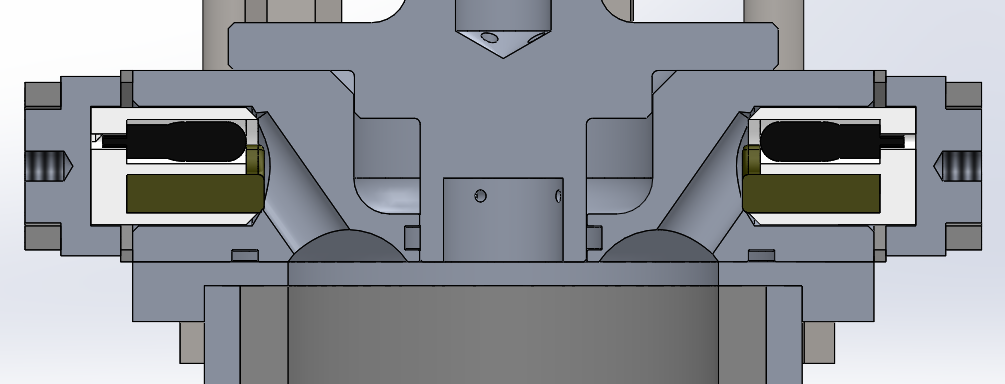
\includegraphics[width=\textwidth]{Propulsion/ignitionCut.png}
\caption{Engine cross section showing the ignition system.\\cartridges: white, e-matches: black, pyro mixture: brown}
\label{fig:sysarch_prop_ignition}
\end{figure}

Two 3D printed plastic cartridges with a diameter of \SI{10}{\milli\meter} and a length of \SI{12}{\milli\meter}, containing an e-match and about \SI{0.7}{\gram} of a mixture of potassium nitrate, sugar and magnesium (i.e. rocket candy with extra sparks) are installed in openings on opposing sides of the engine head, as shown in \Cref{fig:sysarch_prop_ignition}.
Breeches are mounted on top with four screws each, which not only act as gas tight covers but also as electrical contacts to the cartridges. The positive leads of the two igniter outputs of the ECU are connected to the breeches while the negative leads are connected to the engine head. While this arrangement can be a bit annoying at times due to bad electrical contact between the cartridge and engine head and/or breech, it avoids the need for gas tight wire feedthroughs, which caused problems in past designs.

After the e-matches ignite the mixtures, the igniters burn for roughly \SI{5}{\second}. The ignition flames with hot sparks are led into the combustion chamber by angled holes, meeting in the center, below the injector. 

The igniter cartridge installation takes about 10 minutes when done by an experienced team member, and is planned to be done in the prepping area.

\subsubsection{Thrust Chamber}\label{sec:prop_thrustchamber}

The ablatively cooled thrust chamber consists of a casing and a liner with a cylindrical section and a converging-diverging nozzle, bots seen in \Cref{fig:sysarch_prop_thrustChamber}. The conical nozzle geometry is not the most efficient, but allows for simple manufacturing.

\begin{figure}[H]
\centering
\subfloat[Casing]{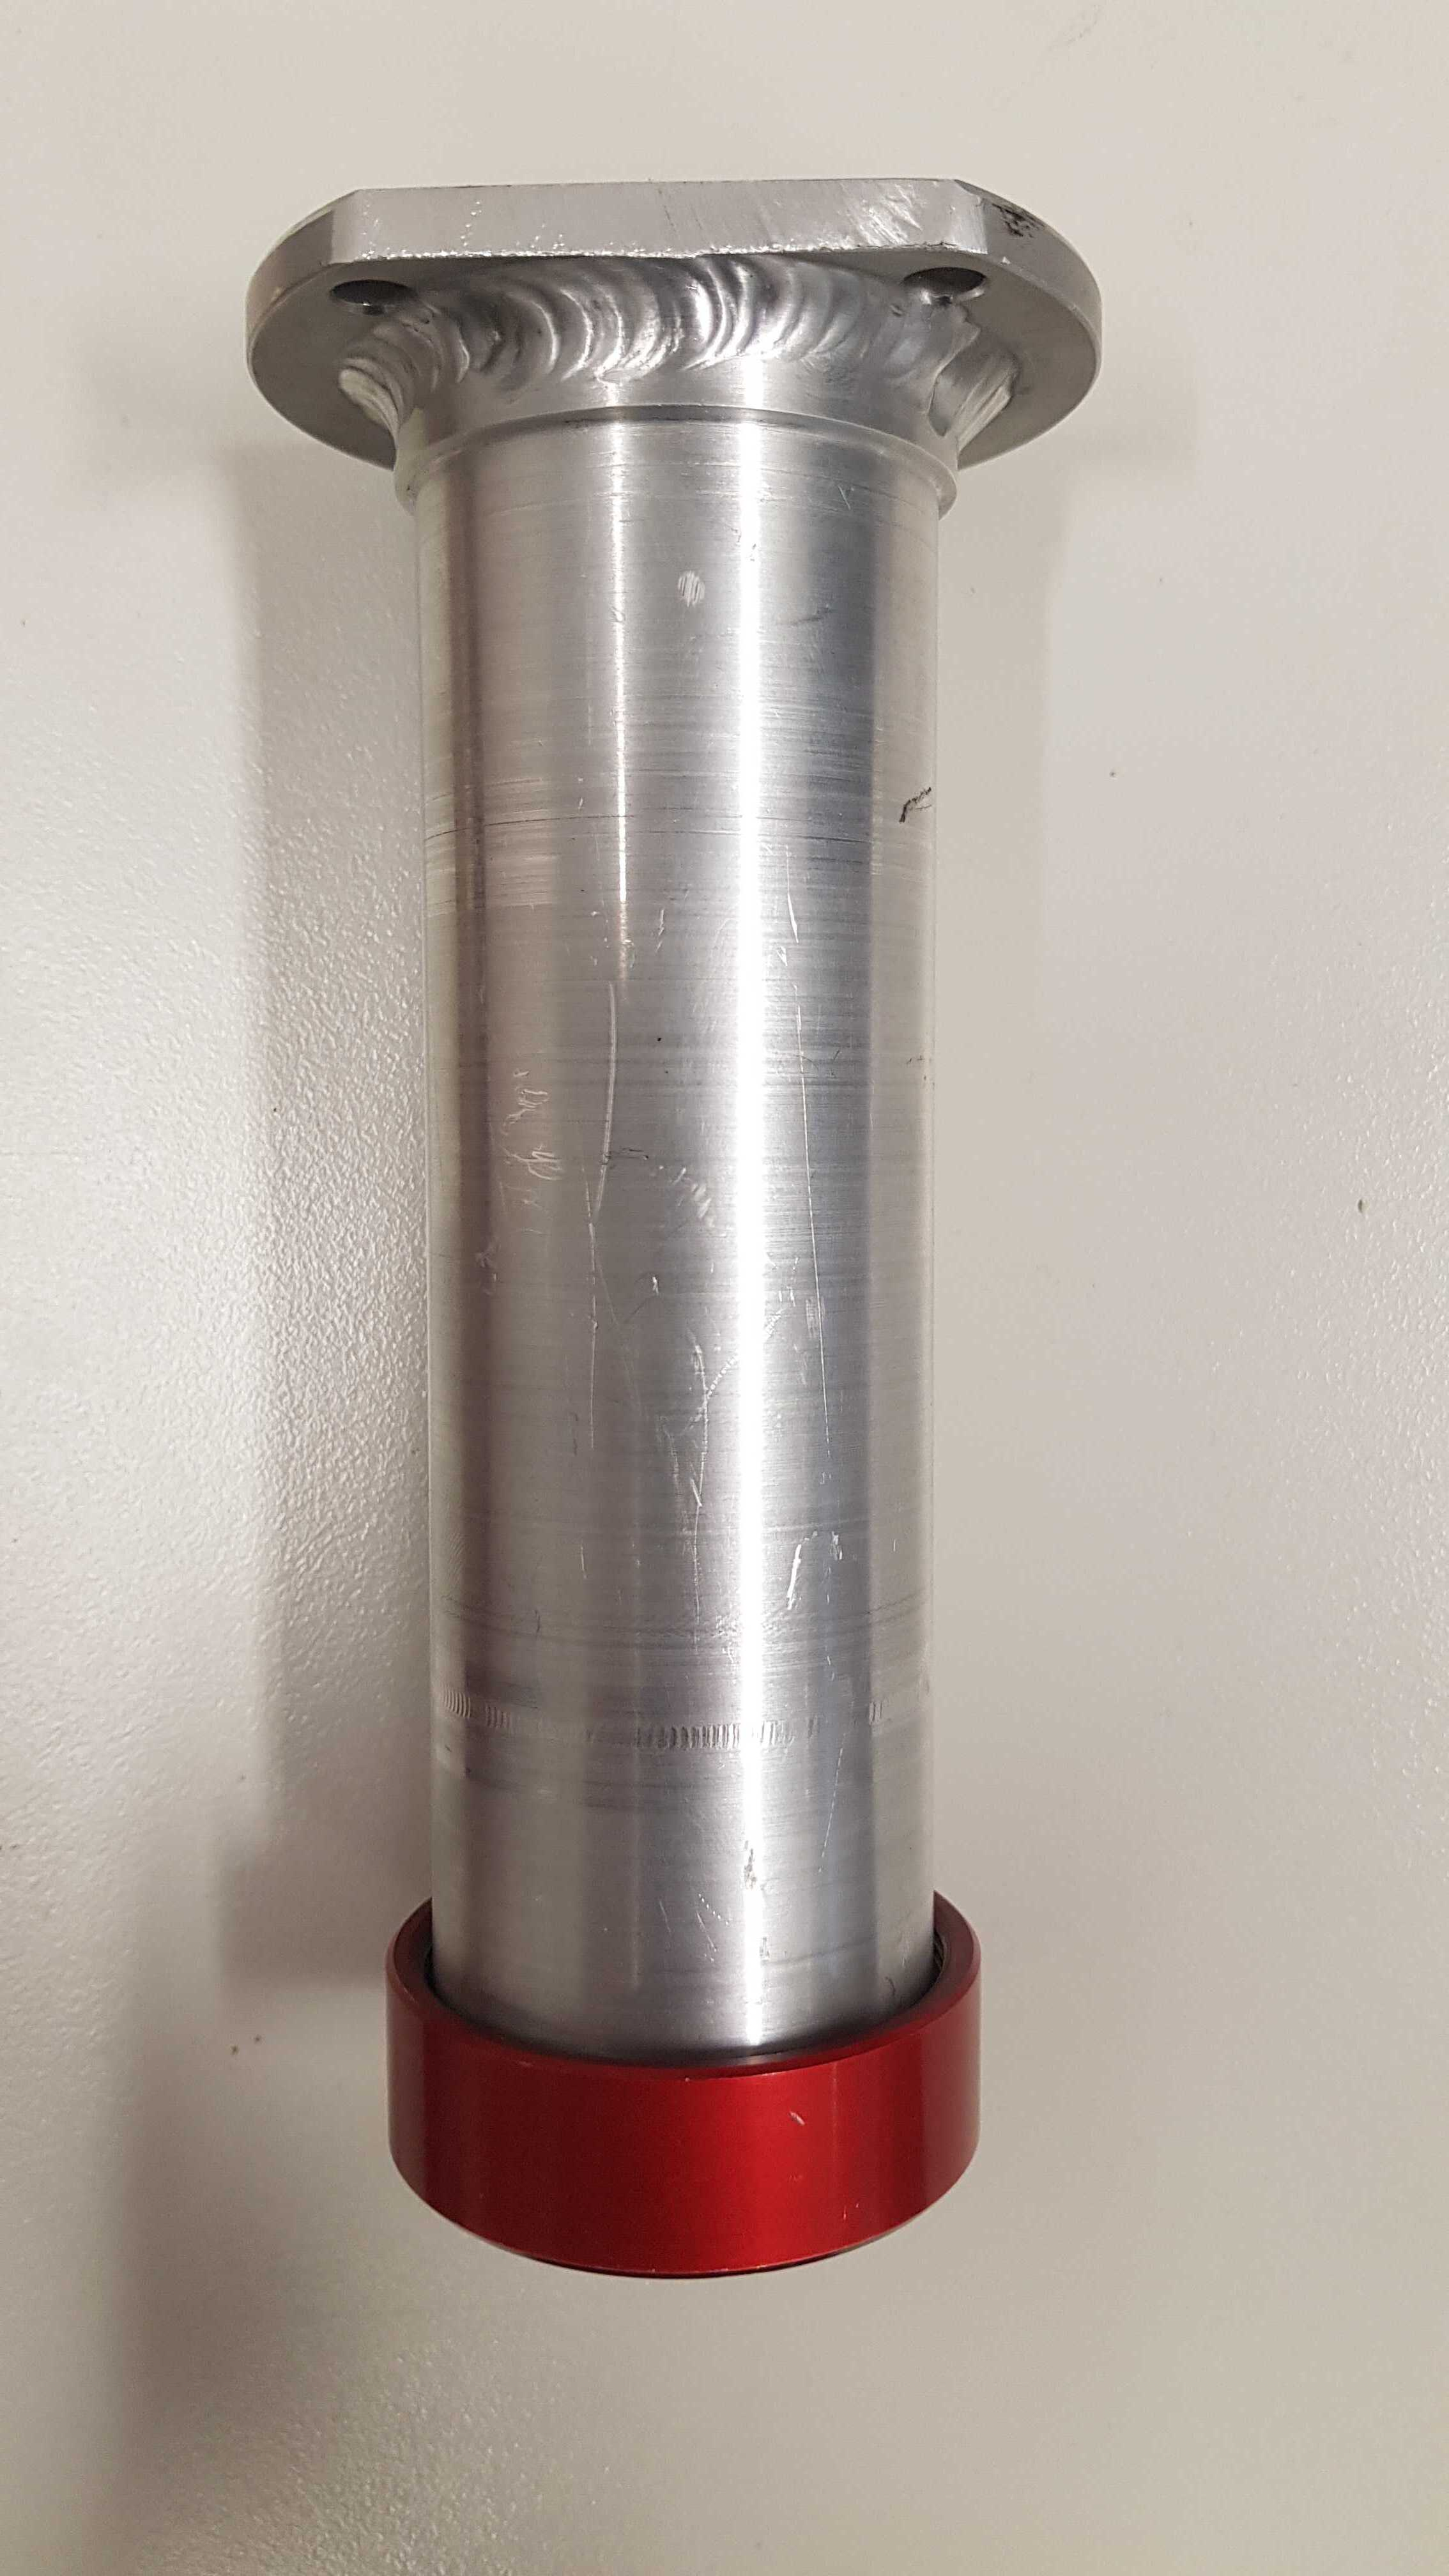
\includegraphics[width=0.3\textwidth]{Propulsion/chamberCasing.jpg}}
\subfloat[Liner]{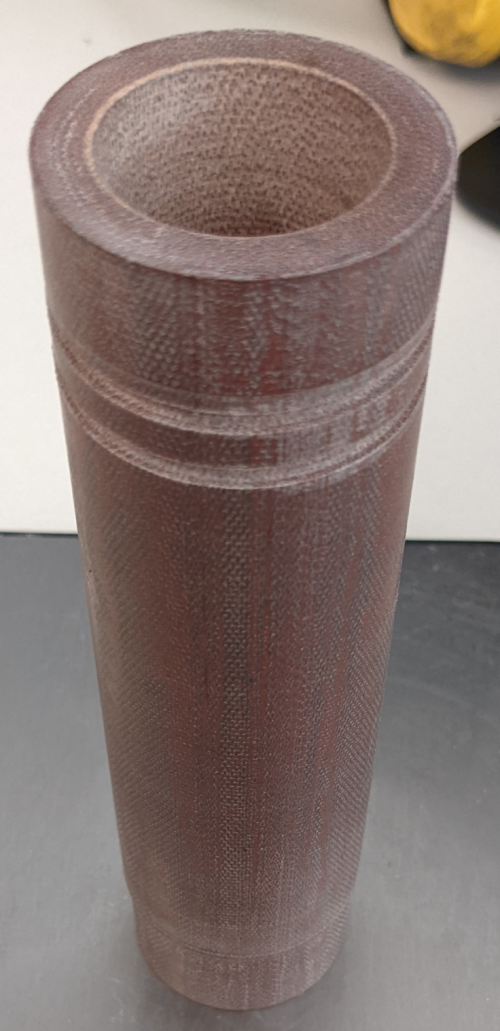
\includegraphics[width=0.3\textwidth]{Propulsion/chamberLiner.png}}
\caption{Thrust chamber}
\label{fig:sysarch_prop_thrustChamber}
\end{figure}

The cooling method was chosen as regenerative cooling is not feasible at this scale (fuel mass flow too low compared to heat flux, cooling with oxidizer is considered complex and risky due to possible decomposition) and film cooling is more complex to implement and increases propellant consumption.

The casing is manufactured from aluminium and consists of a tube section with a flange on one end and an external thread on the other. The flange is mounted to the engine head and sealed with an axial o-ring. After installing the liner, which is sealed to the casing using two radial o-rings, it is held in place by a retainer ring screwed onto the casing.

The ablative chamber liner and nozzle is combined into one component and consists of phenolic resin cotton fabric composite. It is turned out of commercially available round stock, making it a simple, affordable and safe option.

Laminating the thrust chamber from carbon fibre, glass fibre or cotton fabric and liquid phenolic resin was the initial plan, but the procurement of the resin proved to be very challenging. This, together with safety concerns lead to the abandonment of this approach. Using epoxy resins as widely available and safe replacement for phenolics was evaluated, but abandoned after repeatedly delivering unsatisfactory results in hot fire testing.

Cost and manufacturing time could be reduced by switching to a two part ablative design, this was however not pursued for the EuRoC 2022 design due to time constraints. Phenolic paper tubes are commercially available with custom dimensions and lower cost than solid phenolic cotton stock. The manufacturing of the chamber liner would then be as simple as cutting it to length. The nozzle could still be turned from phenolic cotton, but a more viable approach might be to use graphite instead. Using a chamber liner with sufficient thickness and a graphite nozzle would allow the assembly to be used for multiple firings of the engine, while the current one-piece phenolic cotton approach is limited by the high regression rate at the throat.

\subsection{Propellant Loading and Offloading}

\subsubsection{Fuel}

Fuel filling is done manually using a big syringe with a tyre fill adapter connected via a hose, allowing for a precise volume of fuel to be added. The fill adapter opens the check valve completely, allowing the fuel tank to also be drained using the same method. As the ullage gas in the tank needs to flow through the small bleed orifice during filling and draining, significant force on the syringe is needed to finish quickly.

\subsubsection{Oxidizer}\label{sec:sysarch_prop_oxLoad}

Connected to the fill port is the remotely controlled oxidizer fill system described in \cref{sec:groundsys_oxload}.
Oxidizer loading starts by activating the vent valve pressure regulation and setting it to \SI{30}{\bar}. Pressurant is then carefully filled until the vent valve gets activated, after which pressurant filling is stopped. The oxidizer tank is now filled with nitrogen at \SI{30}{\bar}.
Now, the oxidizer fill valve is opened, connecting the oxidizer bottle (cooled down to about \SI{0}{\celsius} to reach a vapor pressure of approximately \SI{30}{\bar}) to the fill port on the vehicle. The pre-pressurization with nitrogen prevents oxidizer from quickly rushing in at this moment, which would be a safety hazard considering the possibility of the nitrous oxide explosively decomposing. Also, the gas phase of the oxidizer in the tank is diluted by the nitrogen, further lowering the risk of a decomposition event. Next, heat is introduced into the oxidizer bottle, leading to a slight rise in vapor pressure. This, in combination with the vent solenoid valve still regulating the tank pressure to about \SI{30}{\bar} (and thus \SI{0}{\celsius}) leads to liquid oxidizer flowing from the bottle into the tank. The displaced gas in the tank gets vented while the heat used in the bottle for evaporation gets replenished by the external heat source.
The completion of the filling process is seen by liquid oxidizer being vented, creating a visible plume, and by the venting frequency changing suddenly. The filling process is stopped by closing the fill valve and deactivating the bottle heating.
If desired, the tank can be topped off by opening the fill valve again (and enabling the bottle heating if necessary), but this is rarely needed as the tank is insulated well and the boil-off rate is thus quite low.

During filling and until pressurization, the oxidizer vapor pressure is regulated to 30bar by the solenoid vent valve. The valve is then kept closed and the pressurant tank filled. The regulator is set to provide a static pressure of 50bar, which drops to 40bar operating pressure as soon as the main valve opens. This active pressurization (“supercharging”) speeds up the launch preparations and prevents cavitation in the feed system.

\subsubsection{Pressurant}\label{sec:prop_pressfill}

Pressurant in the form of nitrogen at up to \SI{300}{\bar} is loaded via the fill ports integrated into the Paintball pressure regulators. During normal flight preparation, the tanks are first partially filled to aid in the oxidizer fill procedure as described above. As the pressurant fill system is shared between the fuel and oxidizer systems, the fuel pressurant tank also gets partially filled in this step. This does not matter though and the system depressurizes within a few minutes through the bleed orifice.

Shortly before liftoff, the pressurant tanks are fully filled after the oxidizer vent solenoid gets switched from pressure control to closed. This is done by opening the fill valve before waiting for the propellant tank pressures to stabilize and then some more to ensure the pressurant tanks are completely filled. After finishing the pressurant fill process by closing the fill valve, liftoff should occur soon to avoid too much pressurant escaping via the bleed orifices. If there is a delay, pressurant can be topped off as long as the fill umbilicals have not yet been disconnected.



\newpage

\section{Aerostructure} %Liana
\label{sec:aerostructure}
The airframe consists of three main parts: the nosecone, the body tube and the fincan. These are connected by aluminium coupler rings, whereby the one that connects the nosecone and body tube is described in detail in the recovery section (\cref{sec:recovery}). Most of the parts are made in-house, so besides the idea behind the design, the process of manufacturing is outlined.

\subsection{Nosecone}
Based on the Von Kármán shape, the nosecone (shown in \Cref{fig:aerostructure_nosecone}) optimizes the airflow around the rocket and minimizes drag. Due to being made of glass fiber, it is transparent to electromagnetic radiation, making it the RF window of the rocket.

The glass fiber mats were wet laminated to a positive 3D-printed mold with epoxy resin in three layers. The surface was then sanded and touched up evenly in several passes before the 3d-printed core was removed.
This \SI{360}{\milli\meter} long center part is enclosed by the \SI{42.25}{\milli\meter} lathed aluminum tip that is screwed into a mounting piece at the top and a aluminium coupler ring serving as a recovery separation mechanism connecting it to the body tube at the bottom, which is described in more detail at \cref{sec:recovery}.

\begin{figure} [H]
\centering
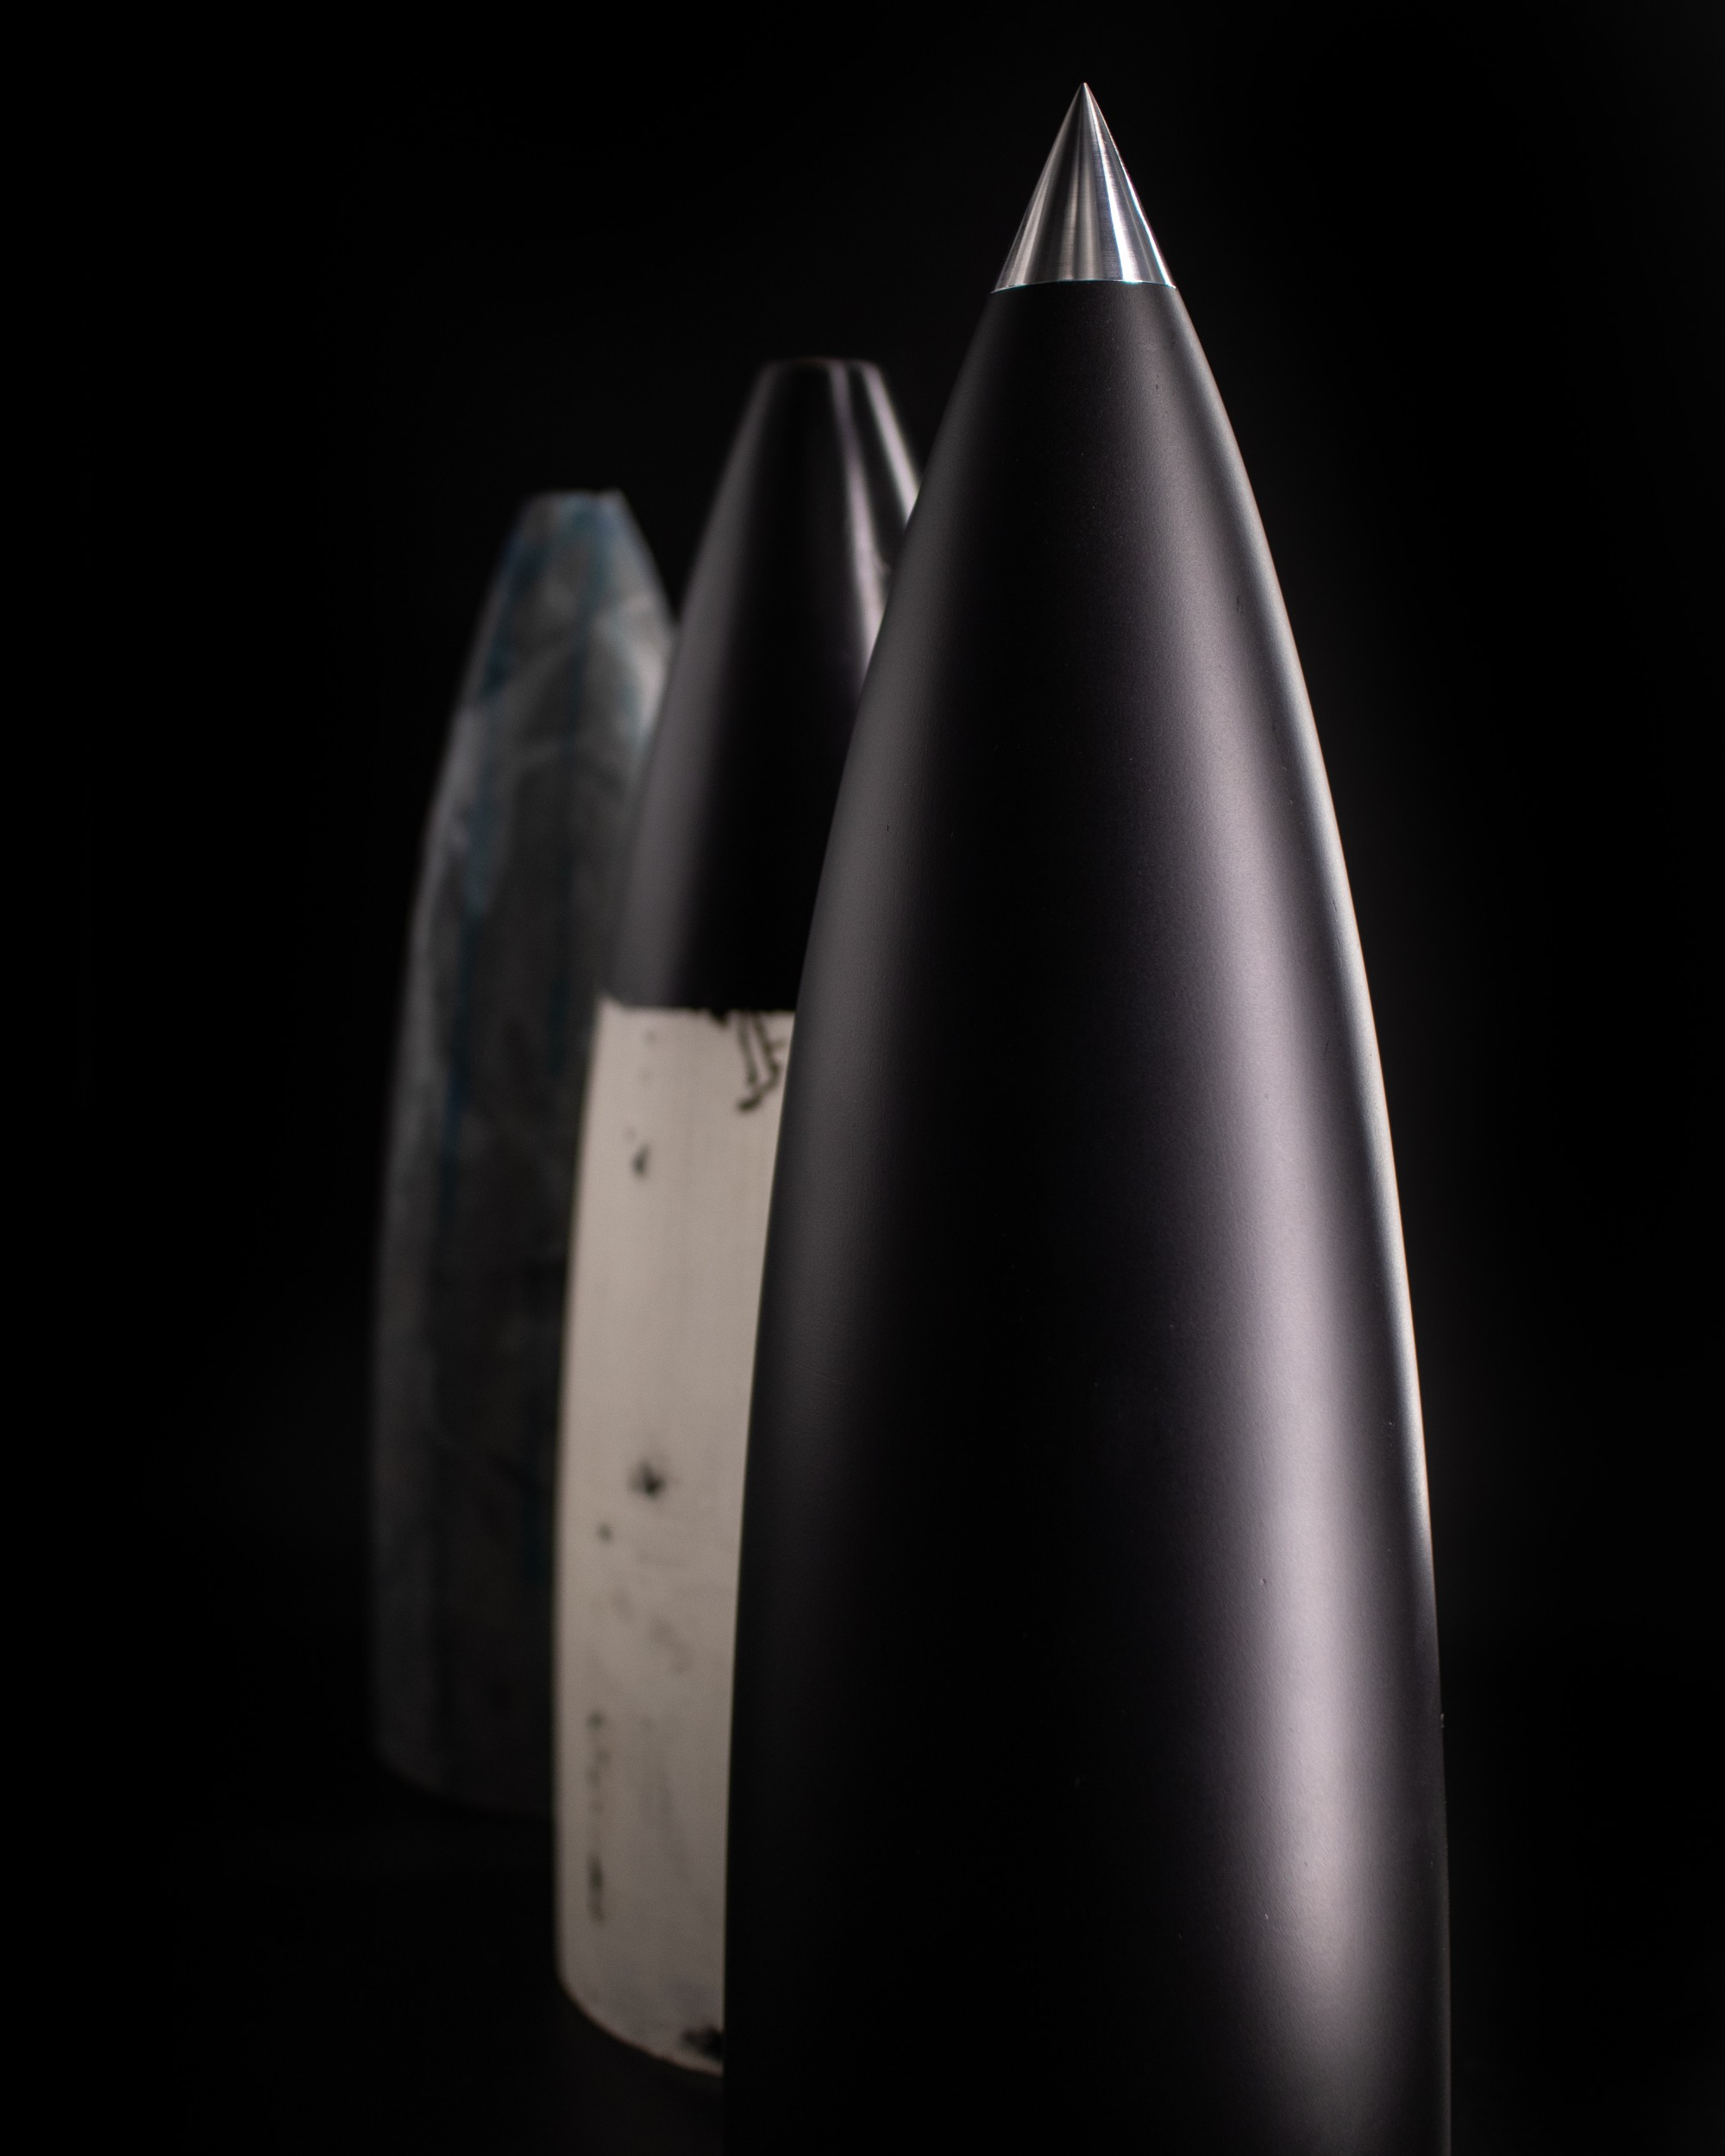
\includegraphics[width=0.5\textwidth]{Aerostructure/NC_4 (2).jpg}
\caption{Different versions of the nosecone, improvements from back to front (final version). The black paint was removed after a test flight and replaced with a white coat.}
\label{fig:aerostructure_nosecone}
\end{figure}

\subsection{Body Tube}
The body tube has an outer diameter of \SI{123}{\milli\meter} and a wall thickness of \SI{1.5}{\milli\meter}. It consists of radially wound carbon fiber inner layers and weaved outer layers and was manufactured to spec externally.

\subsubsection{Umbilical Feedthroughs}
To make fueling, arming and setting up pad-communication convenient, easily accessible connectors and mechanisms are necessary while the rocket is on the launchpad. For this purpose, openings for the connections are provided on the side of the airframe.

\subsubsection{Launch Pad Mechanical Interface}
The vehicle is connected to the launch rail using two rail buttons made of brass. The location of the upper rail button influences both the stability on the rail as well as the effective length of rail available for stabilization during launch. It is mounted with the screw that is also used to hold the fuel tank. The bottom rail button is used to support the weight of the vehicle while on the launch pad and to hold it down until successful engine ignition is confirmed. It is screwed to the airframe fincan coupler.

\subsubsection{Airframe-Fincan Coupler}\label{sec:aerostructure_lowercoupler}
Fincan and body tube are joined using an aluminium coupler ring that provides a tight fit and is held in place via radial screws. This ring is also where the thrust from the engine is introduced into the airframe, using four aluminium struts that connect the coupler ring to the engine head. This is explained in more detail under \Cref{sec:engine_valves_fill_connections}.

\subsection{Fincan}
To bring the center of pressure well below the center of gravity and thus ensure sufficient static stability, we opted for four fins and a lightweight carbon fiber construction. The fillets between fins and center piece are designed rather extensive, so that those areas are resistant enough.

The Fin profile is based on a symmetrical airfoil profile and was then adapted so that a positive mold could be 3D-printed in house. This mold was sanded and treated with several thin layers of coat to seal pores and after that with release agent. Then a four-part negative mold consisting of high-temperature epoxy tooling gelcoat and high-temperature epoxy moulding paste was taken. This was then used to laminate with pre-preg carbon fiber. For the fin cores Rohacell, a closed-cell rigid foam, was chosen. Those inlays are both essential for the stiffness of the fins and ensure that enough pressure is exerted on the laminate during the curing process. The Boards of Rohacell foam were CNC-milled to the correct form and then placed on the four layers of carbon fiber mats before the negative mold was assembled. The inside of the tincan was strengthened with another two layers of carbon fiber. After being sealed in a vacuum bag and cured by by being gradually heated to 135°C in the oven, the fincan was sanded, cut down to the lengh of \SI{300}{\milli\meter} and prepared for painting (shown in \Cref{fig:aerostructure_fincan})

\begin{figure} [H]
\centering
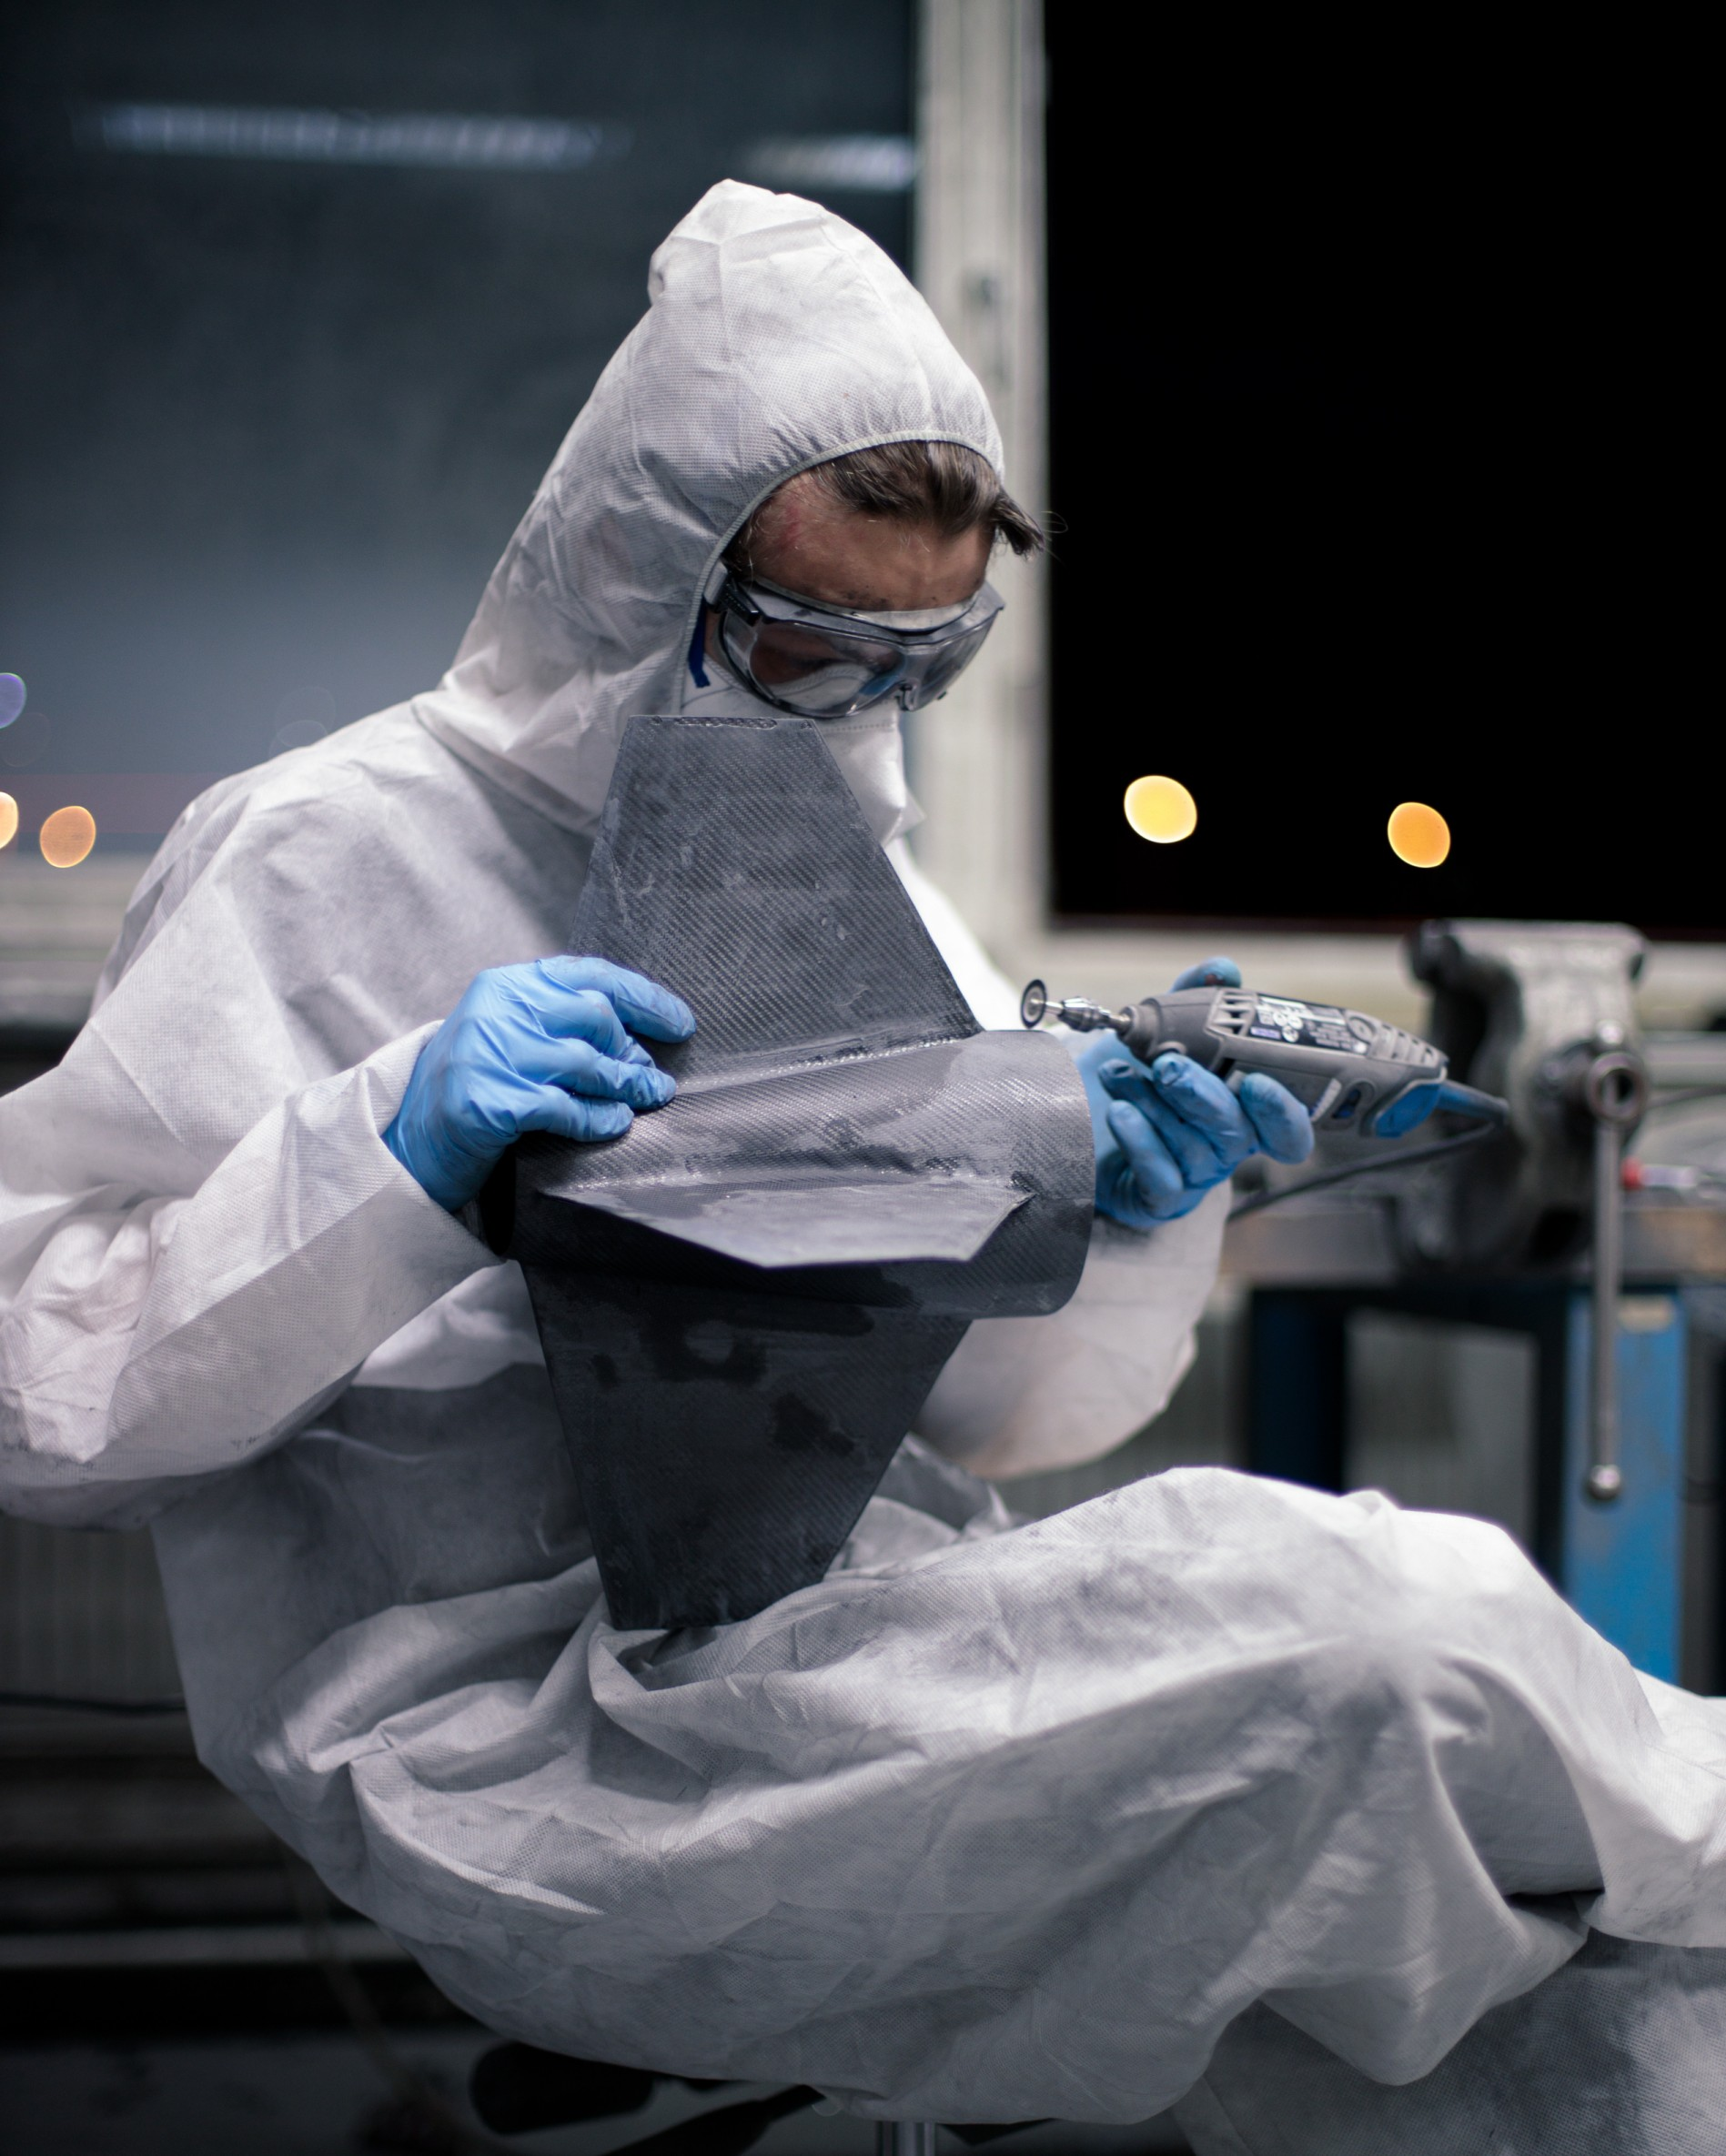
\includegraphics[width=0.5\textwidth]{Aerostructure/Fincan-3.jpg}
\caption{Surface sanding after curing of the Fincan.}
\label{fig:aerostructure_fincan}
\end{figure}

\subsection{Livery Design and Surface Finish}
To accomplish a flawless look as well as create a surface that mitigates some of the solar heating experienced in the EuRoC launch environment, the airframe is painted white. The decision was made in favor of lacquer and against adhesive foil, since the latter has proven to be both unsightly and less resistant. Furthermore, painting allows to not have solid black markings, but to leave the carbon fiber underneath visible, which displays the lamination work and the texture of the airframe.

On the body tube the team name, the project name, the academic affiliation and the sponsor logos are arranged into a minimalistic design. The fins all feature the Team ID and the Austrian flag. Each of them additionally displays a unique but simple graphic pattern of black and white to allow ground-based observers to track and record the launch vehicle’s altitude.

To achieve a satisfactory result, first the flaws were repaired with epoxy resin, then the whole airframe was sanded and coated with transparent primer. After drying, stencil stickers were applied in the places of the markings. The white paint was then sprayed on and allowed to harden. The stickers were then carefully removed and the airframe covered with a clear, matte two-component coat.

\newpage

\section{Recovery}
\label{sec:recovery}

\subsection{Deployment System}

Recovery is accomplished by a two stage parachute system. At apogee, the nose cone is separated from the body tube via our custom designed clamp band mechanism. It consists of two coupler rings (one mounted to the body tube and the other one to the nose cone) tightly clamped together via a spring steel band.

\begin{figure}[h]
\centering
\subfloat[Clamp band Connection]{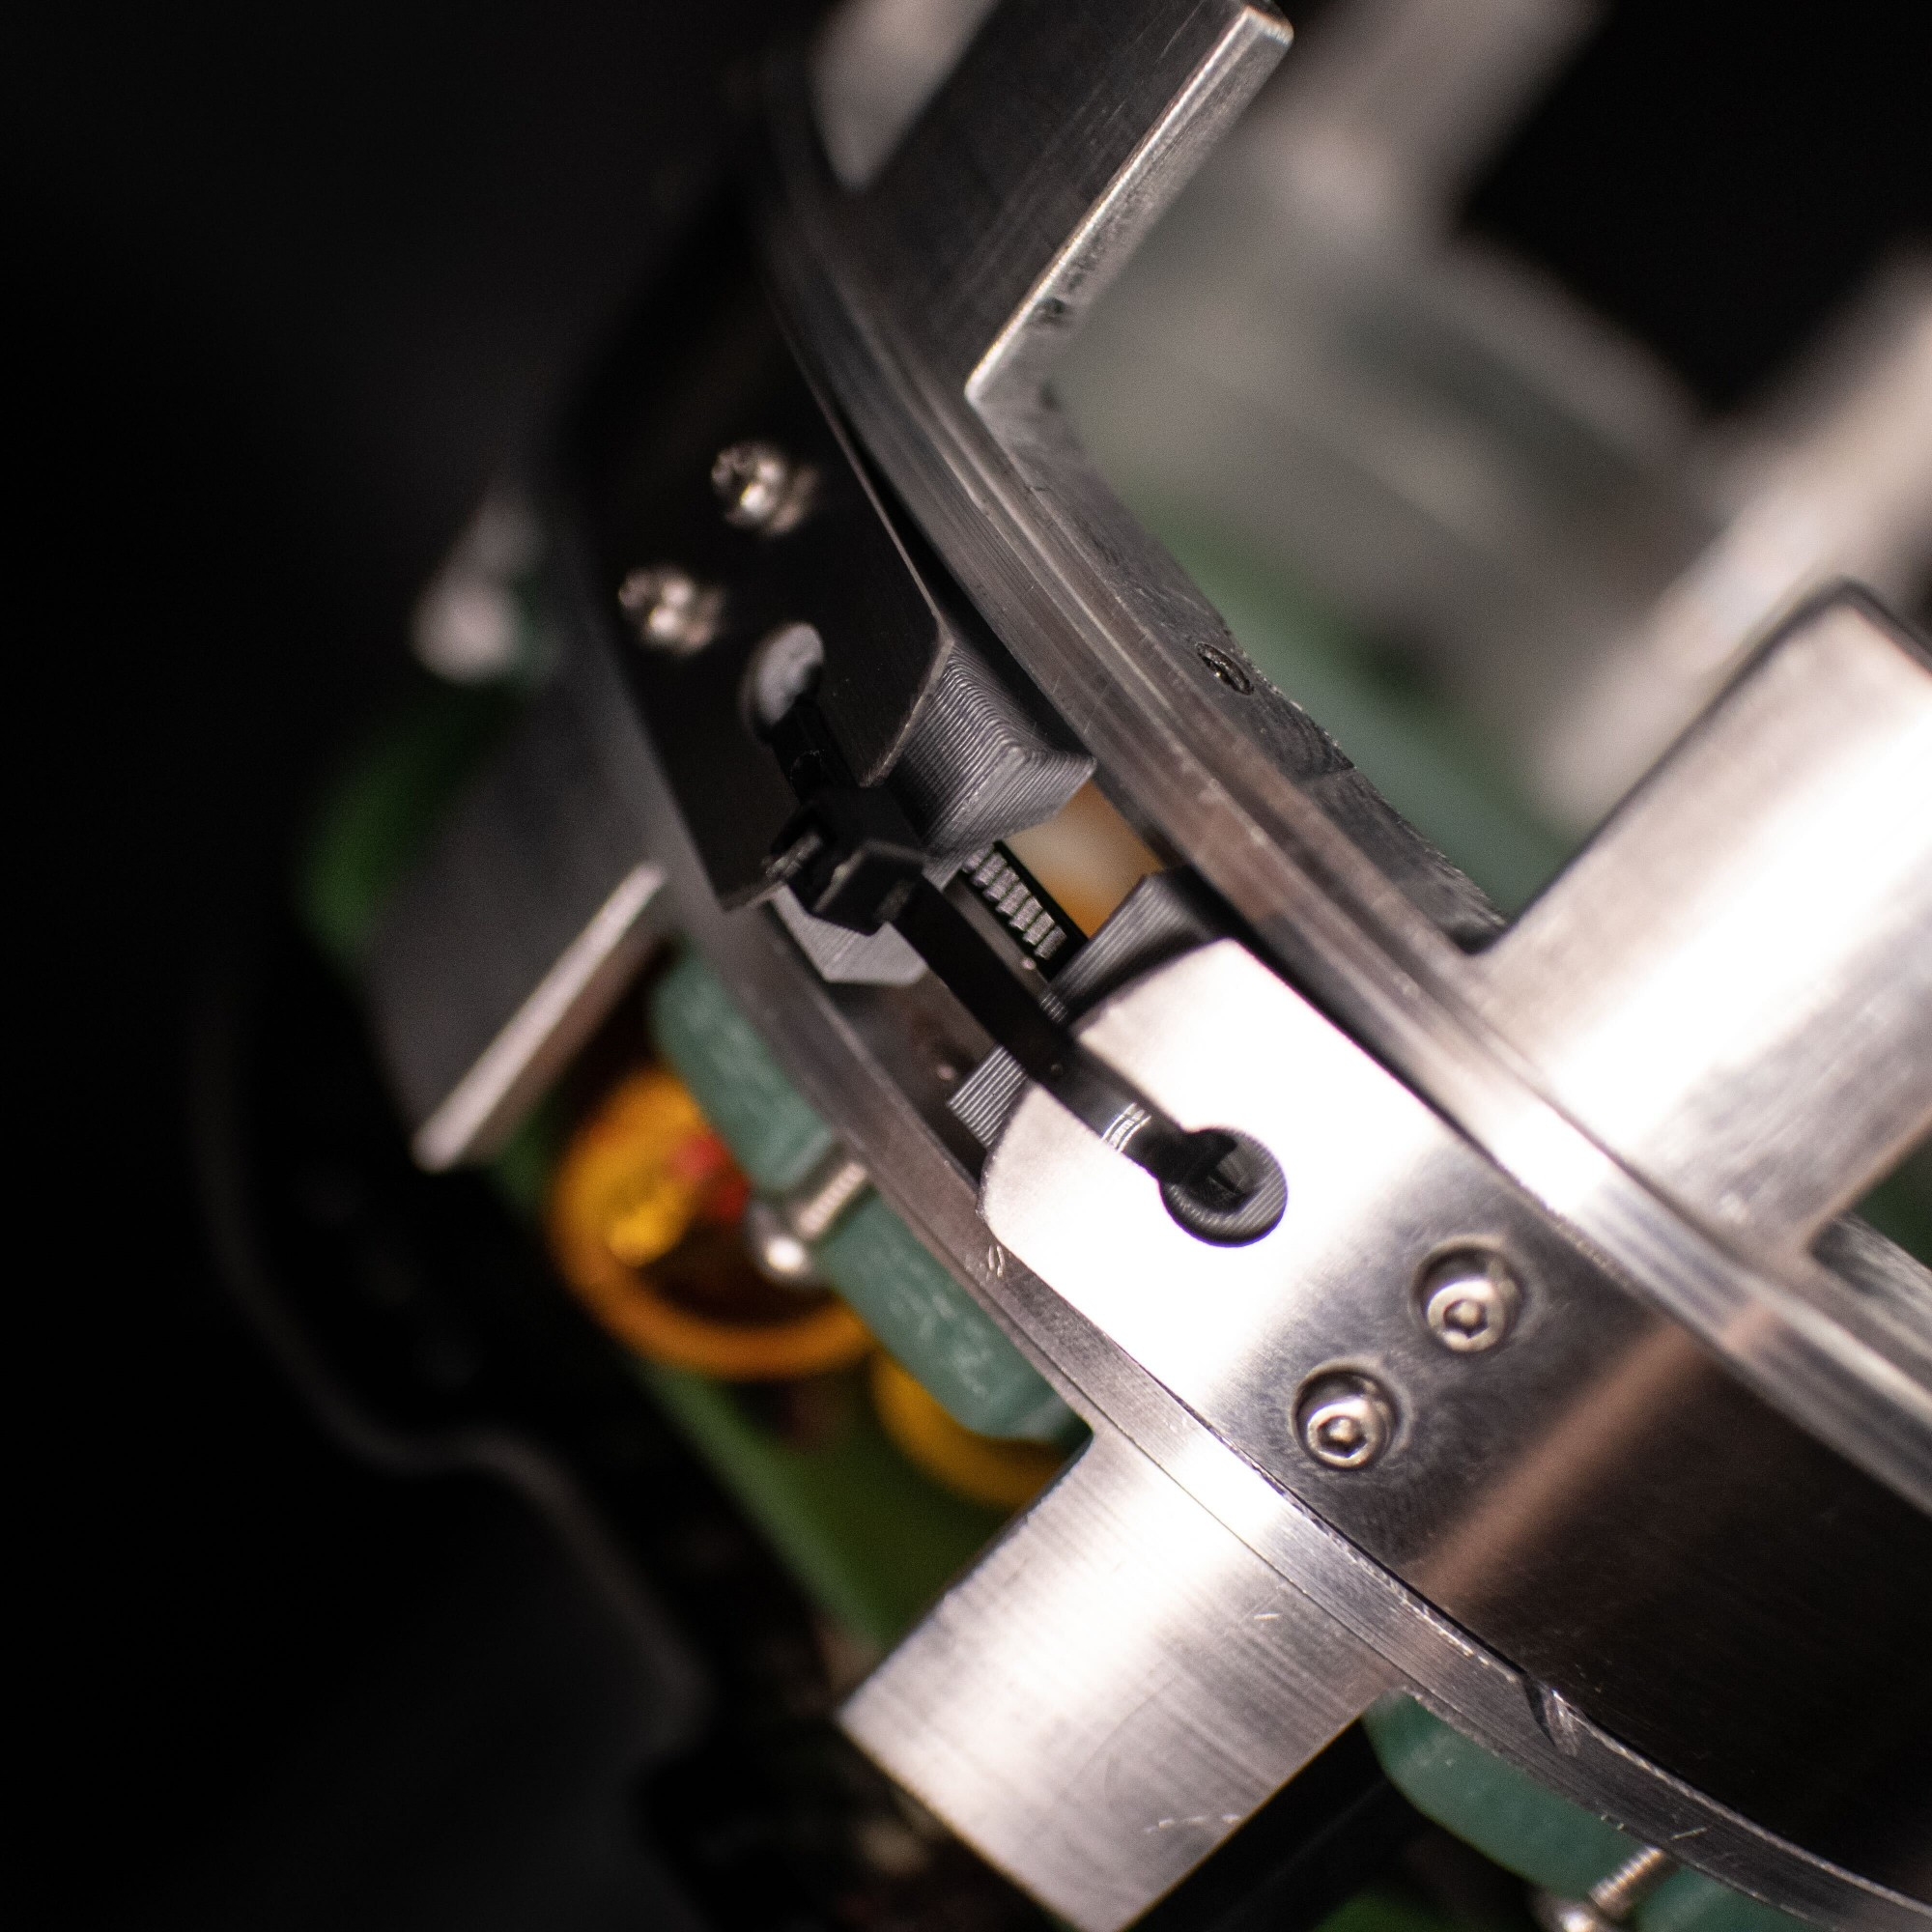
\includegraphics[width=0.4\textwidth]{Recovery/clampband_1.jpg}}
\subfloat[Clamp band coupled to body tube]{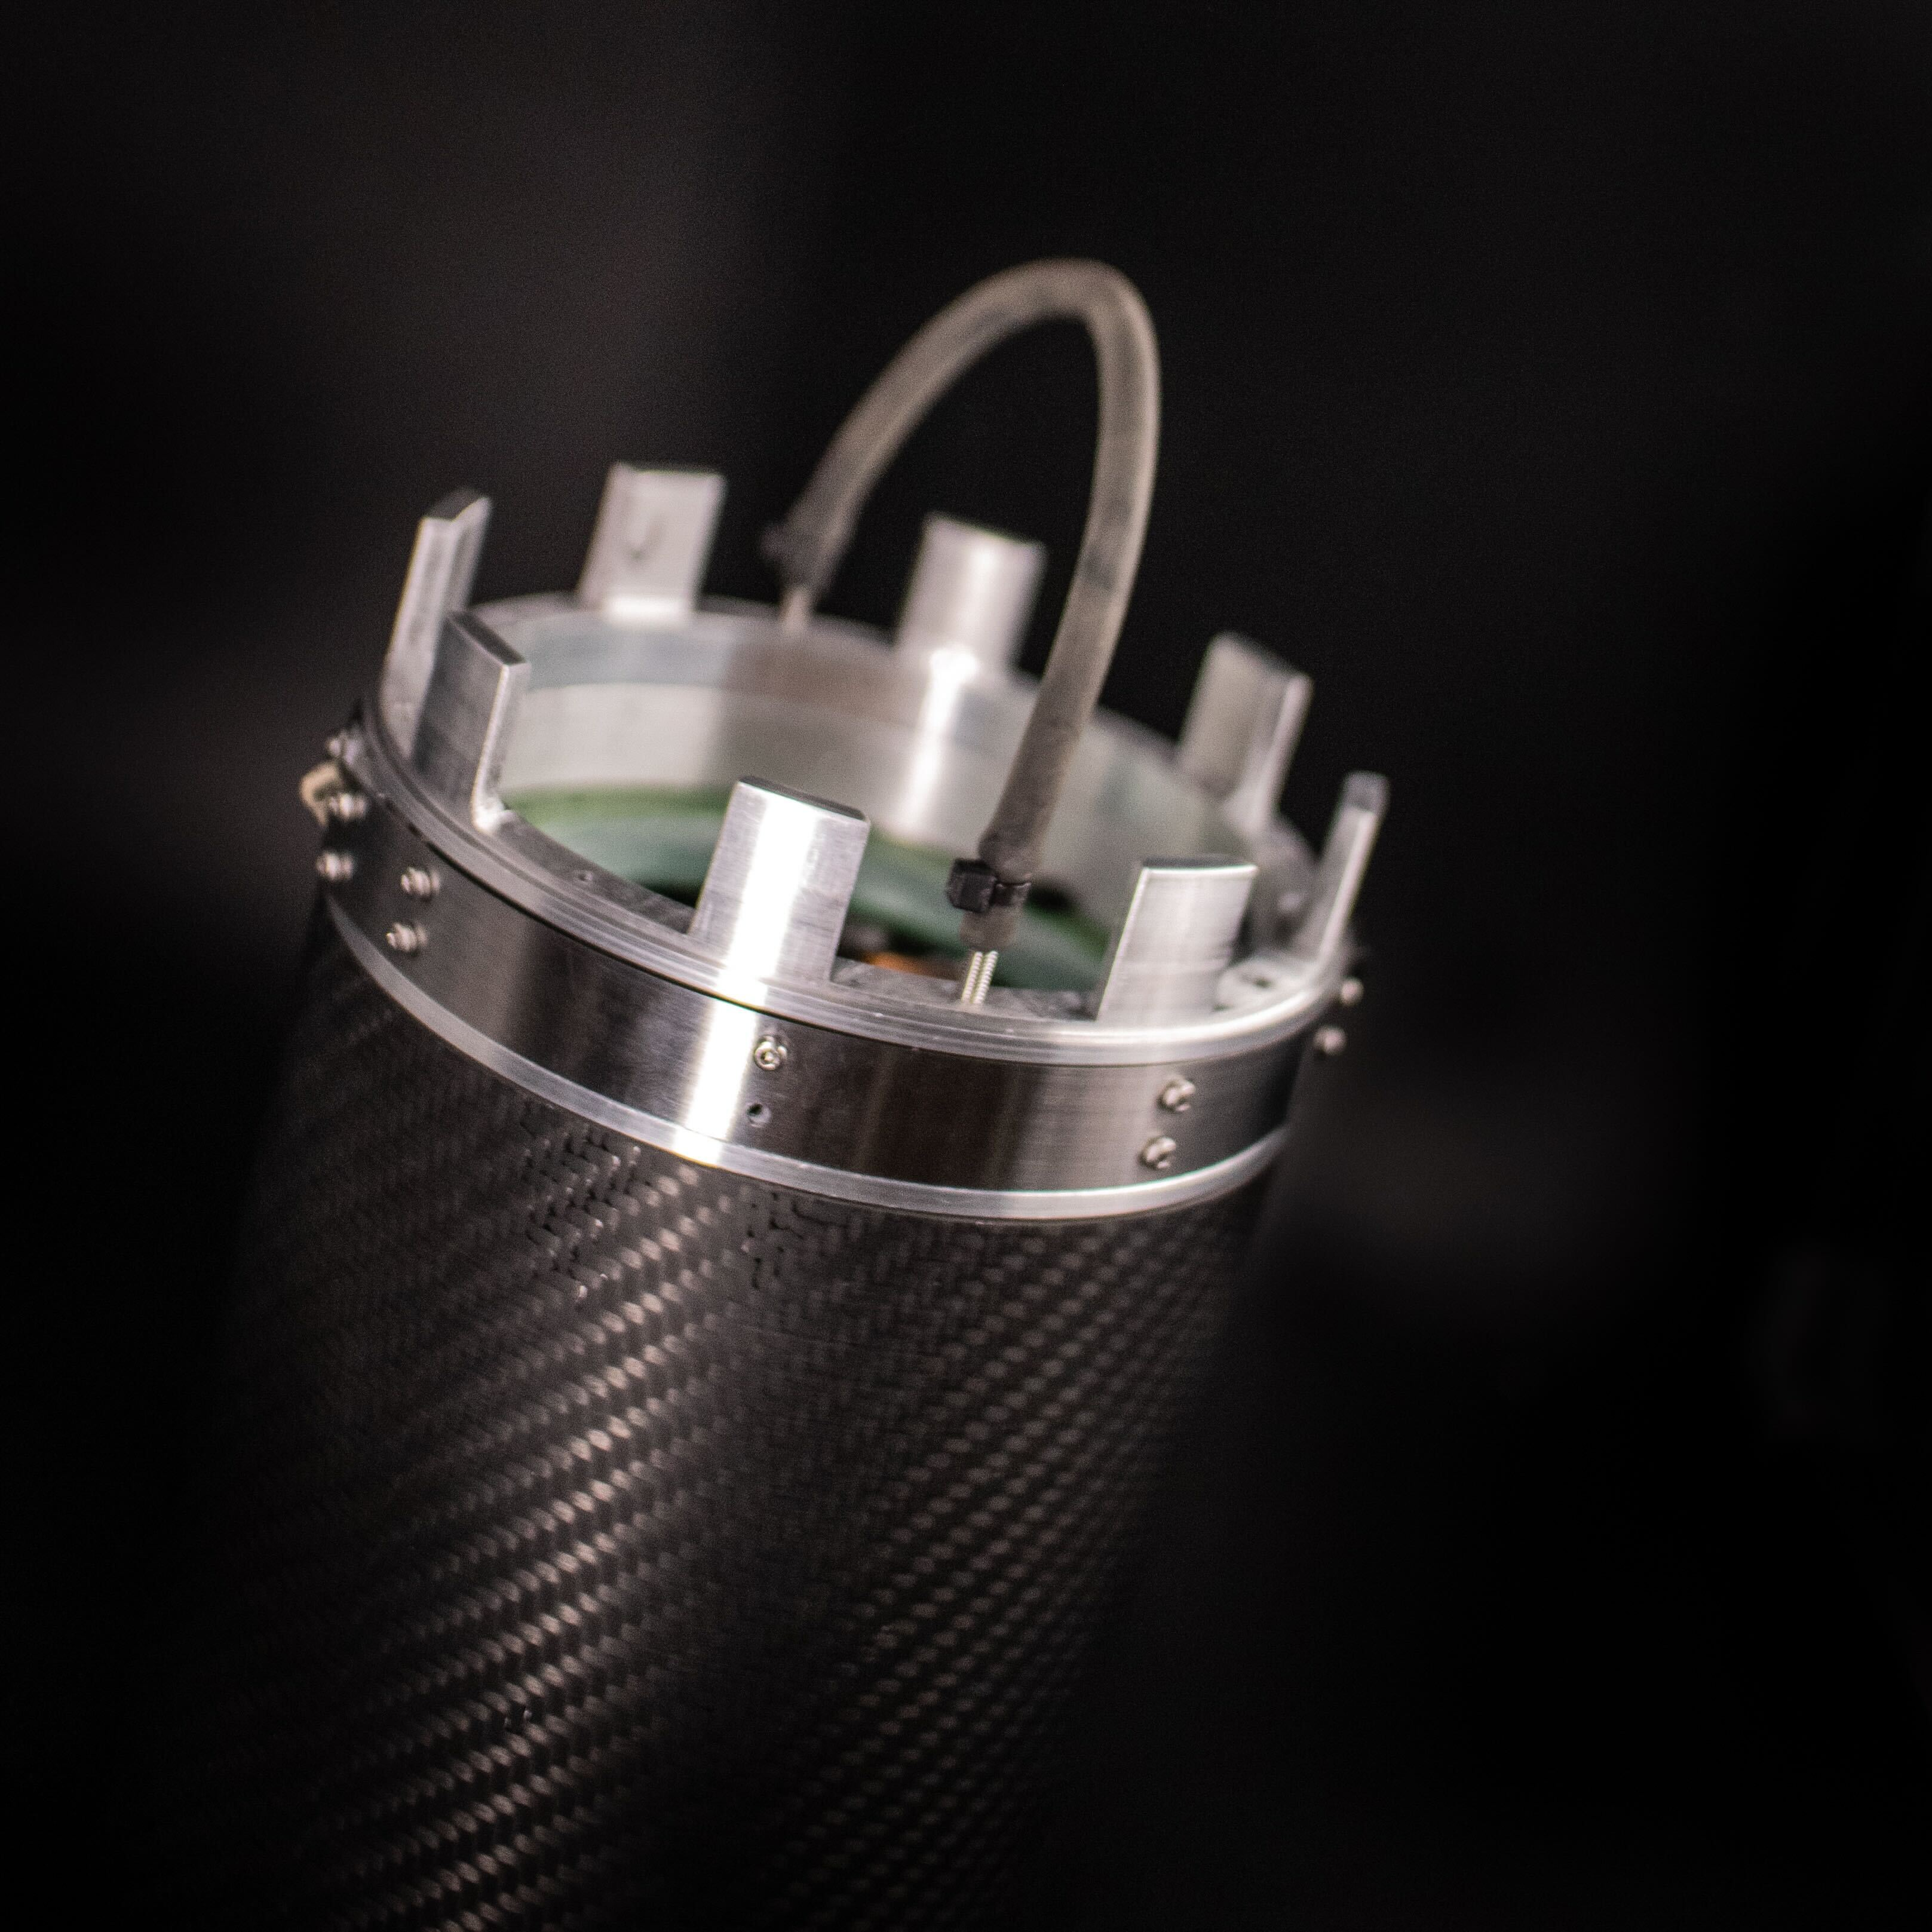
\includegraphics[width=0.4\textwidth]{Recovery/clampband_2.jpg}}
\caption{Clamp band Assembly}
\label{fig:clampband}
\end{figure}

 The clamp band is released by one of two redundant pyrotechnic line cutters severing a line that connects the two ends of the clamp band. The spring steel band separates from the coupler rings (still connected to the main tube by a short line) and releases the connection between them. The coupler on the nose cone is then catapulted away from the bottom coupler ring. This is accomplished by four strong slingshot rubber tubes, ensuring a clean and reliable separation even at high airspeeds (and thus high drag force on the nose cone). Along with the nose cone, a small cup, housing a drogue parachute, is pulled away, releasing the drogue chute.

\subsection{Parachute}

\begin{table}[h]
\centering
\begin{tabular}{ll}
Drogue Chute Diameter & \SI{340}{\milli\meter} \\
Drogue Chute Type & Round \\
Main Chute Diameter & \SI{1400}{\milli\meter} \\
Main Chute Type & Pull-down Apex
\end{tabular}
\caption{Chute Specs}
\label{tab:chute_specs}
\end{table}

During the drogue phase, the vehicle descends quickly (about \SI{35}{\meter\per\second}) and in a controlled manner. The nose cone with the rubber band mechanism and the drogue cup is suspended directly from the drogue with a line shorter than the drogue line to avoid collisions between the nose cone and the body tube. The main parachute and its lines are packed into a deployment bag, which is housed in a cup mounted to the lower section. A few hundred meters above ground, a second set of line cutters severs the connection between the drogue line and the vehicle and another line that keeps the main deployment bag from sliding out of its cup. This puts tension on the line connecting the drogue line and the main deployment bag, allowing the drogue to pull out the main deployment bag. Tension on the main line opens the deployment bag, allowing first the lines and then the parachute to be pulled out of it in a controlled manner. The rocket now descends at about \SI{7.6}{\meter\per\second}.
In this final landing configuration, the drogue and nose cone assembly stay connected to the deployment bag and main parachute. The system has been successfully validated in multiple ground tests, and in a test launch to \SI{700}{\meter} using a mockup airframe propelled by a solid motor. Small modifications are planned to increase reliability and to allow for easier assembly/preparation. Additionally, the parachute sizes will be adapted to the increased vehicle mass.

\subsection{Failure during Test Flight}
On our most recent test flight of the rocket, the recovery has failed by the drogue chute line ripping during the initial drogue deployment. With the rocket then being in free fall the main chute line never had a chance of holding. After carefully studying the received data and video footage of the test flight, the failure has been identified to most likely be caused by the following: The wind speeds encountered at launch day were higher than expected, leading to a higher horizontal velocity at apogee. This of course means that the airspeed, when deploying the drogue, was higher, increasing the load on the lines. Additionally, quite thin drogue lines were chosen based on pre-existing knowledge and experience within the team, which in conjunction with a drogue that was too large and a non-functional shock absorber lead to the lines snapping.
These issues will be rectified in the new recovery system for EuRoC. Since all of the identified causes of the recovery failing have been eliminated and a successful recovery test flight (not using our liquid propulsion, instead having a dummy solid booster) was conducted, we are confident that the recovery system will perform nominally for our flight at EuRoC.

\newpage

\section{Payload}
\label{sec:payload}

\uH's payload is part of STS1 (SpaceTeamSat1), a different TU Wien Space Team project. SpaceTeamSat1 is a 1U cubesat, its primary mission is to design and build a cubesat completely in-house that will eventually fly orbit in space and survive the conditions there. The secondary mission of STS1 is to give students the opportunity to run their own Python scripts in space. The scripts are executed on a Raspberry PI CM 3+, which is connected to several sensors via an I2C bus. The sensors include temperature, magnet, gas, acceleration and more.

\begin{figure}
    \centering
    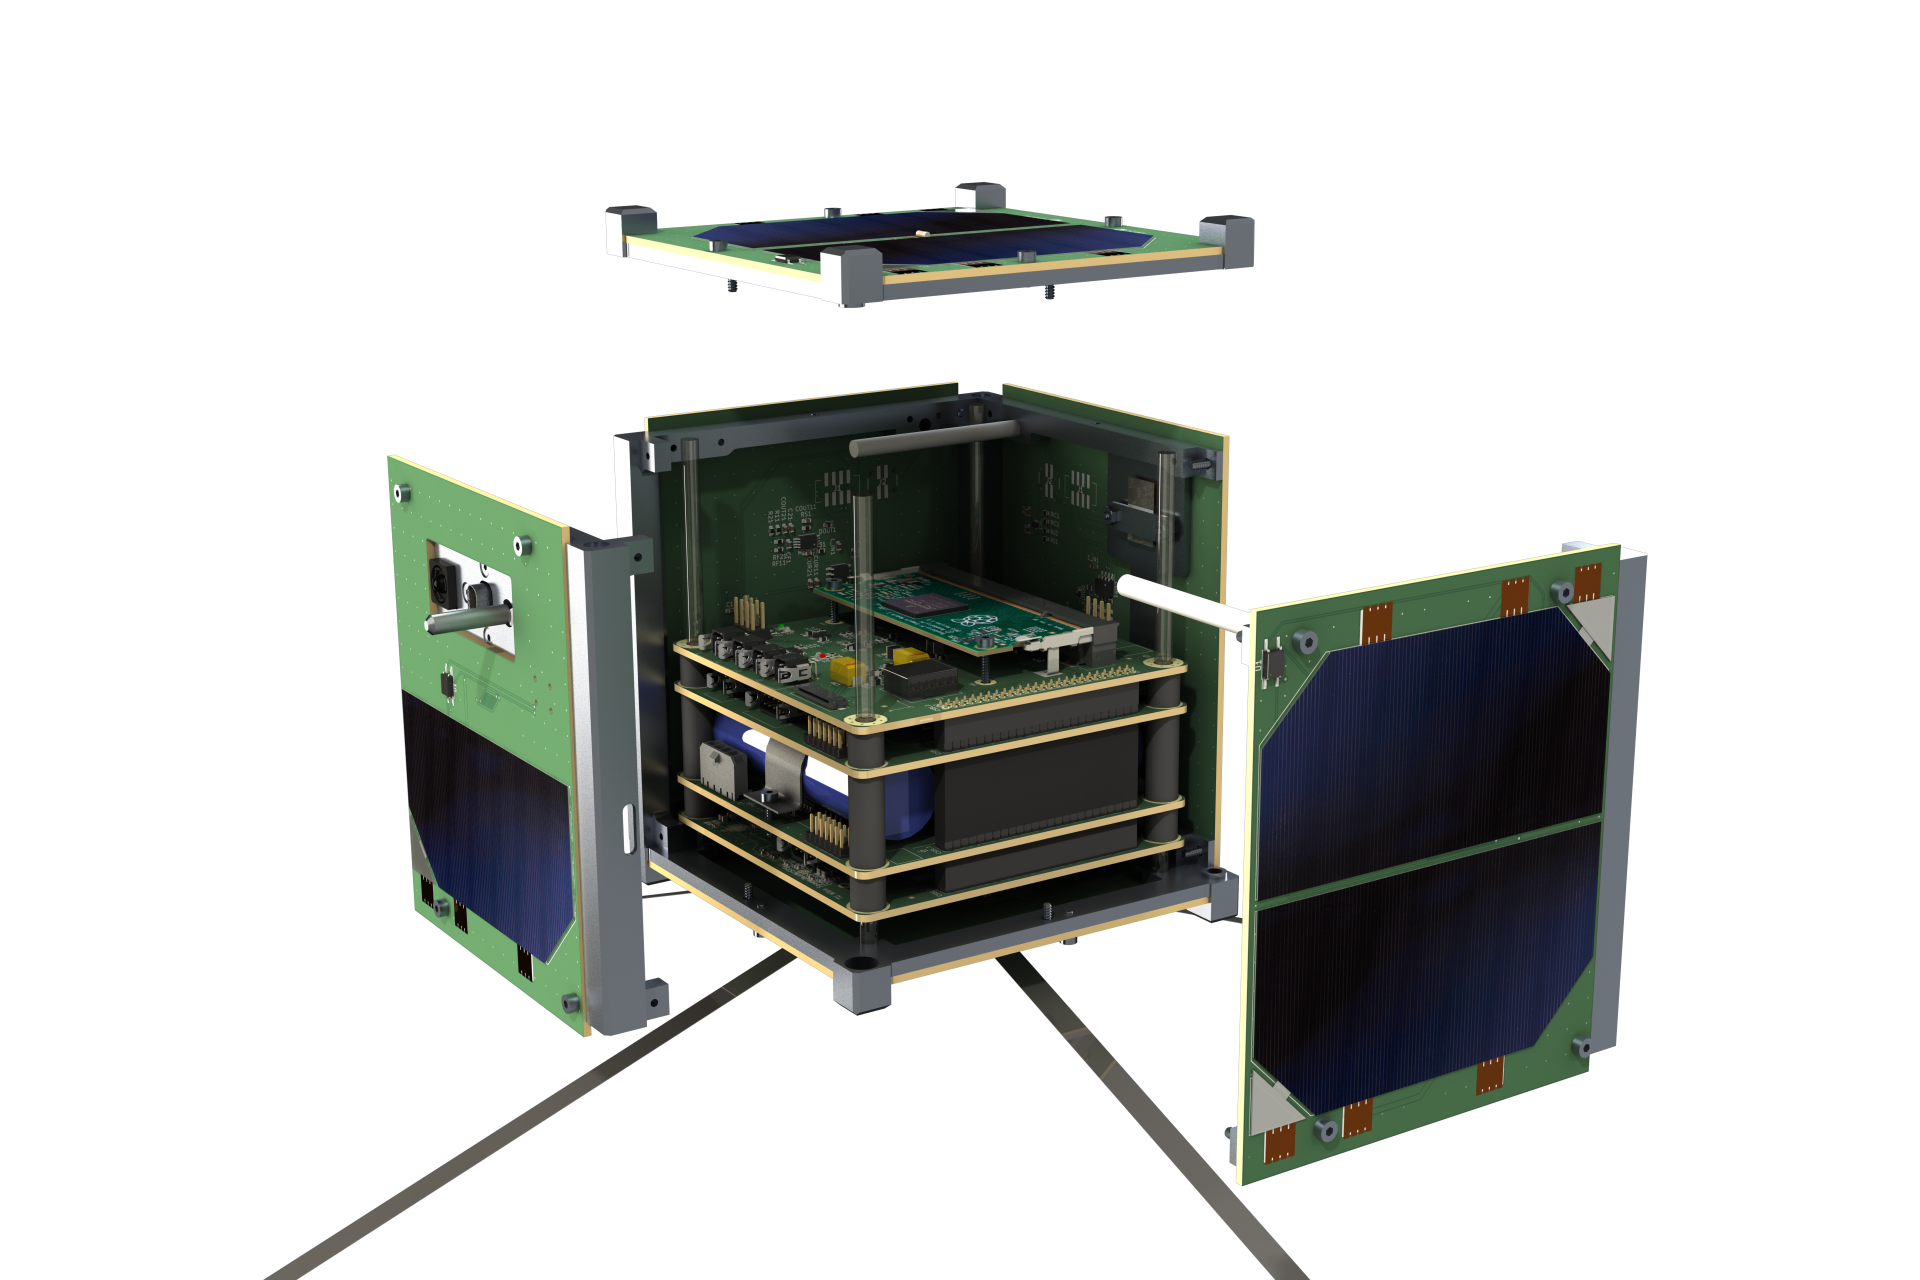
\includegraphics[width=0.7\textwidth]{Payload/STS1_Payload.png}
    \caption{Payload: STS1 Render}
    \label{fig:payload_render}
\end{figure}

This inter-project collaboration offered itself as the \uH launch is a great opportunity to flight test some of the hardware for the cubesat and because \uH needs to fly a payload anyways. Since the full 1U cubesat wouldn't fit inside the \uH airframe only the EDU subsystem is going to be flown.

To fulfill the internal goals for the payload the education subsystem of STS1 and a power supply is required. The whole assembly is installed in a \SI{100}{\milli\meter} x \SI{100}{\milli\meter} x \SI{50}{\milli\meter} housing with a total mass of \SI{1}{\kilogram}, this meets the requirement of four PocketSats with a mass of \SI{250}{\gram} each.

\newpage

\section{Avionics}\label{sec:avi} %Paul, Markus, Lukas

It is advised to read section \ref{sec:software} in 
advance to fully comprehend the following content.

\subsection{Subsystem Block Diagram (SSBD)}
The avionics subsystem is divided into multiple different modules as shown in \cref{fig:avi_ssbd}. 
Those include the three custom designed ARM based units: ECU (engine control unit), PMU (power management unit) and RCU (radio control unit), two COTS Altimax G4 altimeter as well as the mandatory Eggtimer TRS. 

\begin{figure}[H]
    \centering
    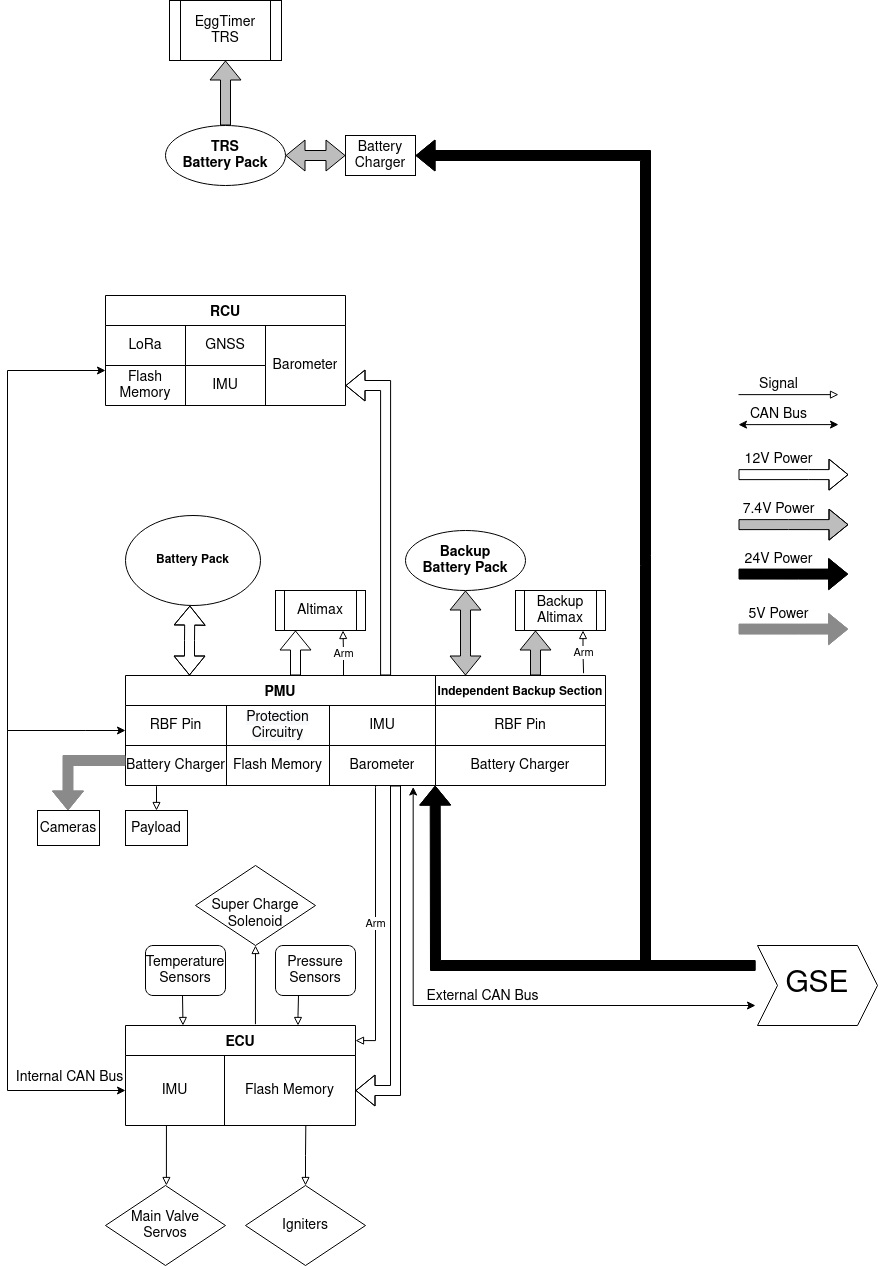
\includegraphics[scale=0.4]{Avionics/Avionics_Blockdiagram.png}
    \caption{Subsystem Block Diagram, see \cref{fig:gse_ssbd} for the block diagram for the GSE}
    \label{fig:avi_ssbd}
\end{figure}

\subsection{Physical Architecture}
The following section describes our three custom units, all equipped with an ARM processor and two CAN-FD interfaces: \textbf{ECU}, \textbf{PMU} and \textbf{RCU}.

The ECU (engine control unit) contains all the electronics necessary for the liquid propulsion system. This includes circuitry for controlling the main valve servos, the supercharge solenoid as well as the igniters. It also has inputs for the chamber and tank pressure sensors, for the tank temperature sensors and current and servo position feedback. A \SI{32}{\mega\bit} external NOR-flash-chip allows for the logging of all data packets sent to mission control in full sampling speed. This is especially useful during flight, where the data transmission speed is limited by the LoRa communication.

The PMU (power management unit) is powered by a 3S1P Li-Ion 18650 and features over-current protection, voltage and current monitoring. It also contains an IMU and a barometric pressure sensor for redundancy reasons, and logs all its data to flash memory. The PMU interfaces with all the other avionics, supplies them with power and bridges between the two CAN-FD busses. Located on a separated part of the PCB, an independent backup section powered by a backup battery pack charges and arms the backup Altimax Altimeter. Moreover, the PMUs RBF (Remove before Flight) pin circuit switches on the igniter voltage, carried to the ECU on its own power cable, separately, allowing an ECU power-up without ignition capability and, thus, ensuring that the ECU can not activate the igniters in operation modes, where the pad crew is present.

The RCU (radio communication unit) consists of communication and sensing hardware. A GNSS module, an IMU and a barometric pressure sensor collect important data for recovery and post processing. Again, all data is logged to external flash memory. A \SI{433}{\mega\hertz} LoRa module sends data to the ground station.

\subsection{Operational modes}

Safe:
Once the rocket is mounted the RBF pin is pulled halfway, which powers on all avionics onboard. At this point data is redundantly sent via \SI{433}{\mega\hertz} LoRa and the rocket can be fully controlled by our Mission Control software via a \SI{2.4}{\giga\hertz} directed radio link, the only exception being the ignition, which is still physically disconnected from power by the RBF pin. Thus,  the final pad preparations including fueling and preparing oxidizer filling are done in this mode.

Armed:
Once the on-pad preparations are done and the pad area is vacated, the RBF pin is pulled out completely, which exposes the ignition circuitry to power. The whole system is now operational. When the launch window opens oxidizer filling begins, marking the last event before launch.

Internal Control:
After oxidizer loading is completed the rocket is put into internal control, where the ECU begins its internal sequence.

Holddown:
If neither hold nor abort is commanded by the operator or the ECU, the ignition sequence is automatically started. After ignition the holddown clamps are still engaged holding the rocket firmly on the launchpad. The rocket stays in holddown mode until sufficient engine performance is detected by measuring combustion chamber pressure.

Lift-off:
If suitable chamber pressure is detected by the ECU, it commands the launch pad to release the holddown clamp. The rocket leaves the launchpad, disconnecting the electrical umbilical cord, and, thus, the power and CAN connection to the launch pad. This leaves us with only the unidirectional LoRa communication. The rocket is now fully controlled by the ECU. 

Powered Ascent:
During the powered ascent phase, data is being sent to Mission Control at all times. At the end of the planned burn time, the ECU closes the main valves to shut down the engine, also known as Main Engine Cutoff (MECO).

Unpowered Ascent:
With the ECU having finished it's internal sequence, the SRAD avionics only remain active to transmit data, shifting focus towards the COTS altimeters detecting apogee.

Recovery:
Once apogee is detected, the two-phase recovery begins with the ejection of the nose cone and drogue chute. This marks the last operation mode of the rocket. See \cref{sec:recovery} for more details on the recovery process.

\subsubsection{Pre-Launch Sequence}

The Pre-Launch Sequence is conducted on our self developed Web-Client.
It contains a dynamic and interactive Piping and Instrumentation Diagram (P\&ID/PnID) for monitoring and controlling all components, the tanking system as well as avionics inside the rocket. A checklist is carefully being processed that states each step needed for preparing and tanking the rocket for launch. Each step is announced by the Launch Commander and is re-validated and executed manually by Mission Control. At T-10 seconds internal control is activated and the rocket self-checks for any malfunctions during engine startup and launch.

\subsubsection{Abort Sequence}

In case of any malfunctions during engine startup either the internal control system can abort or Mission Control can send an abort to the rocket manually. In either case the main valves are instantly closed to prevent any thrust generation. After that a separate checklist is conducted manually to revert the system back to a safe state.

\subsubsection{CAN protocol}

To establish a steady communication with ground systems as well as the rocket, the CAN-FD protocol is used. The whole setup is split into three busses that are all connected to an Ubuntu server. Since the CAN bus is disconnected from the rocket at lift-off, a separate internal CAN bus is used to maintain communication between ECU, RCU and PMU. The PMU is able to bridge CAN messages between the internal and external CAN busses. A self developed protocol is used on top of the CAN-FD protocol to establish the controllability and flexibility needed for Mission Control.

%\subsection{Failure Analysis}

%\subsubsection{Module failure scenarios}


%\subsubsection{Testing strategies}

\newpage

\section{Ground Systems}
\label{sec:gndsys}
\subsection{Launch Pad} %Johnny

For the launch pad, the newly constructed Space Team launch pad will be used. It is large enough to fit all ground system components and with a new rail extension the now \SI{7}{\meter} launch rail is long enough to allow the rocket to take off at a decent speed. Since it is already built, it saves time and resources which would be required to construct a new one, specific to \uH. \cref{fig:gro_lp} shows the launch pad in usage.

\begin{figure}[H]
    \centering
    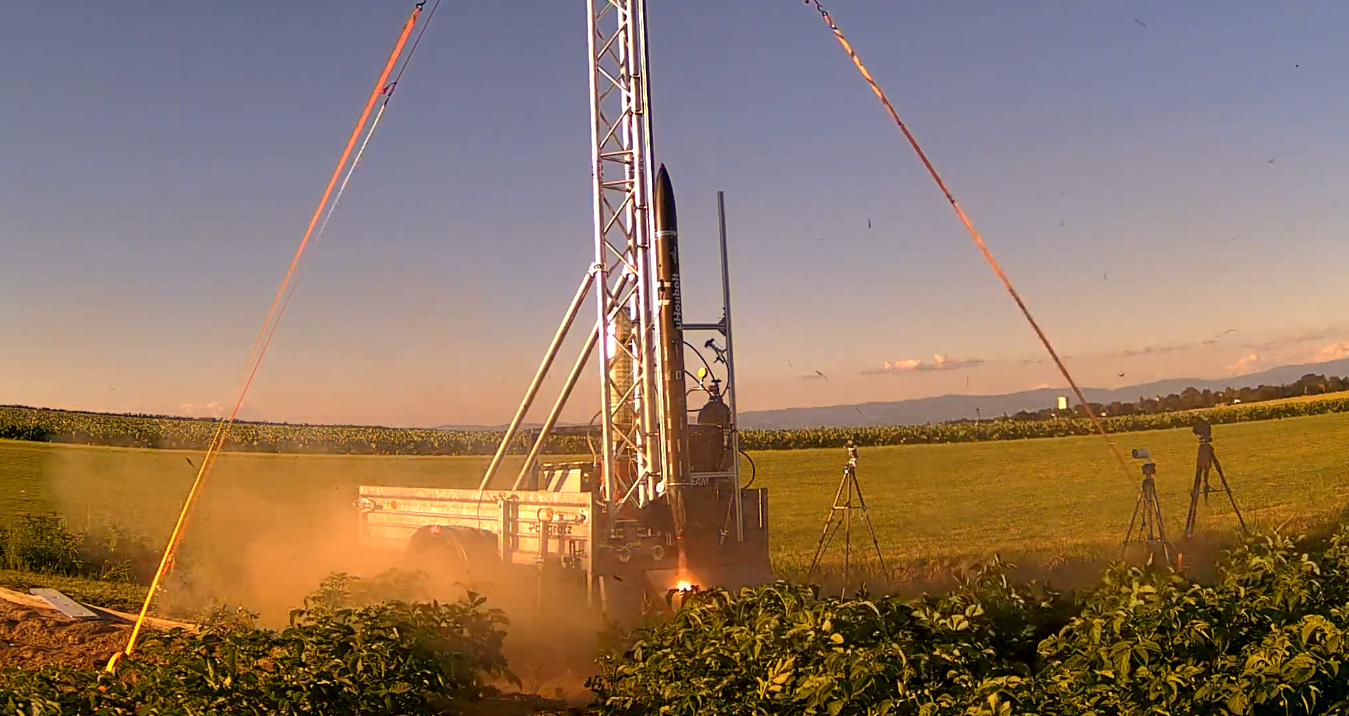
\includegraphics[width = \textwidth]{GroundSystems/uhb_on_rail.png}
    \caption{Launch Pad with \uH during lift-off on first test flight}
    \label{fig:gro_lp}
\end{figure}

\subsubsection{Rail}
The launch rail consists of pieces of 30x\SI{30}{\milli\meter} aluminium extrusion profile, each mounted to one corner of a section of triangular aluminium truss. Pipe clamps screwed into one side of the profiles are used to connect the profile to the truss sections. The whole rail consists of  three truss sections, two of them measuring \SI{2.5}{\meter}, one at \SI{2}{\meter}, which are connected by slotting the ends of one section into the ends of the previous section and securing them with cross bolts. The extrusion profiles on top are then aligned using long sliding blocks in the lateral grooves, resulting in a seven meter long continuous launch rail. The rail buttons on the rocket ride in the dorsal groove.
One of the truss sections is mounted to the launch pad trailer using hinges. This allows the lowest rail section to be folded down during transport. For a launch the other two rail sections are added and the whole rail, once in the upright position, is braced against the trailer as well as guyed to the ground. See \cref{fig:gro_lp}.

\subsubsection{Holddown} \label{sec:holddown}
While the rocket will be guided along the rail using rail buttons its vertical movement will be restricted by an additional holddown system. Two bars are placed on the top and bottom of the lower rail button. The top bar is connected to a pivoting mechanism, while the bottom bar is connected to a plate with a force measurement system. By measuring the weight of the rocket while tanking the fill level of the oxidizer tank can be estimated. During the ignition sequence, the upper bar of the holddown system prevents a premature liftoff. As soon as the chamber pressure (and thus the thrust) is high enough, the system unlocks the pivoting mechanism with a COTS RC servo motor and releases the rocket. This ensures that a liftoff can only happen when the engine performs as expected and accelerates the vehicle to a velocity sufficient for aerodynamic stability when leaving the launch rail. It also offers an additional abort scenario in case of a loss of control over the fuel or oxidizer valves by constraining the rocket to the launch rail for the entire burn duration.

\subsection{Tanking Infrastructure}

The tanking infrastructure (containing oxidizer and pressurant loading system) is mounted on the trailer next to the launch rail. It contains all the necessary plumbing and electronics to remotely tank oxidizer and pressurant and disconnect the umbilicals before the launch.

\begin{figure}[h]
    \centering
    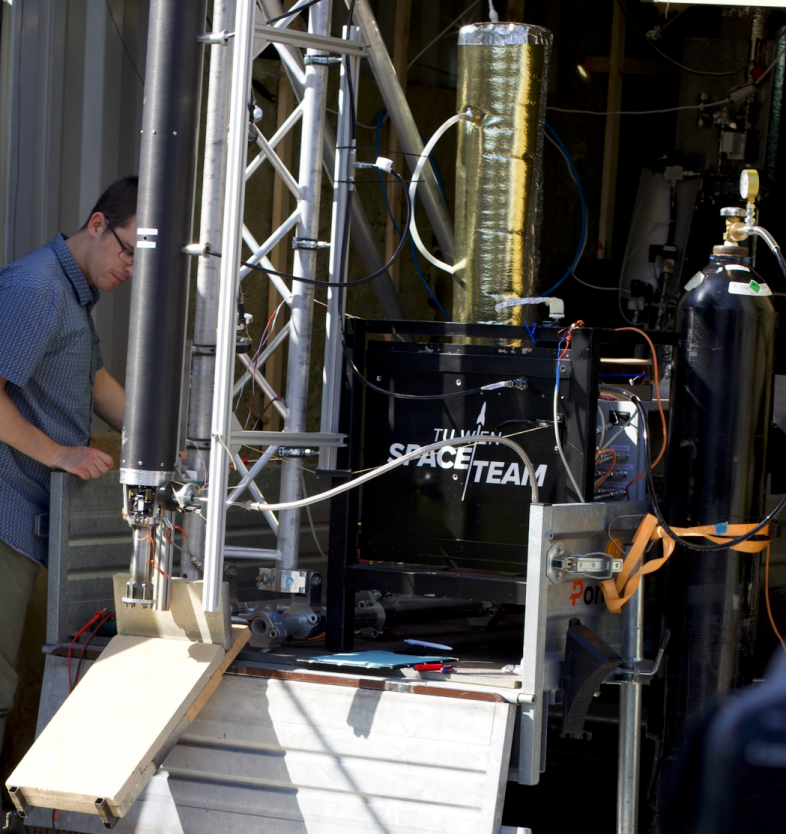
\includegraphics[width=0.5\textwidth]{GroundSystems/gse_uhoubolt.png}
    \caption{Rocket on rail (left) and oxidizer \& pressurant loading system (right)}
    \label{fig:gse_umbilicals}
\end{figure}

\subsection{Oxidizer Loading System}
\label{sec:groundsys_oxload}

See \cref{sec:sysarch_prop_oxLoad} from the Propulsion chapter for a more complete description of the process. This chapter mostly focuses on the physical setup. For a piping diagram see \cref{fig:full_pnid}.

Nitrous Oxide is supplied from a standard gas cylinder which is mounted upside down in the propellant loading system. A heat exchanger jacket is placed over the cylinder in order to be able to control its temperature. In cooling mode the jacket is supplied with water slightly above \SI{0}{\celsius}, while in heating mode the water has \SI{30}{\celsius}.
The hot and cold water is stored in two insulated tanks on the back of the propellant loading system.

This heat exchanger jacket mostly consists of a modified PVC drainage pipe.
To install the gas cylinder the bottom flange of the heat exchanger jacket is placed upside down on the bottle neck, with the valve sticking through a hole in the flange and secured using a nut which fits the threads normally used for the bottle cap. The cylinder is then turned on its head and the bottom flange inserted into a cradle on the propellant loading cart where it is secured using cross pins. Then the jacket is installed and fastened to the bottom flange using three toggle latches around its outside. Lastly the cooling/heating system is connected to the heat exchanger using two hoses equipped with quick-connect fittings. The feed line enters the heat exchanger on the bottom while the return line exits it on the top.

At this point the nitrous oxide cylinder can be connected to the oxidiser loading system and the oxidiser and pressurant umbilicals can be connected to the rocket. Before the start of actual oxidizer loading the tank inside the rocket needs to be pre-pressurized with nitrogen which uses the same pressurization system as the final pressurization before launch via the pressurization umbilicals.

After completion of the filling process (indicated by liquid being vented through the solenoid valve instead of gas), the fill valve is closed. Opening a vent valve in the oxidiser loading system depressurizes the umbilical in preparation for its remote controlled detachment. This is needed as the quick disconnect fittings in use for the umbilicals can't be remotely disconnected under pressure. The entire oxidizer loading process starting from opening the fill valve to the oxidizer tank being full takes about one minute.

The pressurant fill system then supplies nitrogen from a standard \SI{300}{\bar} cylinder to the two pressurant tanks in the vehicle. Same as the oxidizer loading system it also uses two valves for filling and umbilical venting, but it does not need a temperature management system.

%This is achieved by holding the N2O bottle at a temperature of at least \SI{10}{\celsius}. The tank in the rocket will be colder than this, because some of the nitrous oxide already in the rocket will be bled off to reduce the temperature, using the same effect as is tried to counteract in the source tank with the heating.

%It is imperative to not increase the temperature too much, because nitrous oxide goes critical at \SI{36.5}{\celsius} which encourages the spread of decomposition processes (due to e.g. impurities) of the nitrous oxide which is a big safety risk.

The individual steps that need to be executed during the filling procedure are listed in section \ref{sec:oxidizer_loading}.

\subsubsection{Temperature Control}
Switching between the heating and cooling cycle is facilitated by actuating two 3-way valves, one in the feed line, one in the return line and only turning on the hot or cold water feed pump.

The water in the heating cycle is brought to temperature using a \SI{3}{\kilo\watt} water heater controlled by a temperature sensor inside the hot water reservoir, while the cooling cycle temperature is maintained by periodically dumping dry ice into the cold water reservoir. Although water ice can also be used if dry ice is not available, using dry ice is the preferred option, since it doesn't influence the water level in the system.

\subsubsection{Electronics Components}

\begin{figure}
    \centering
    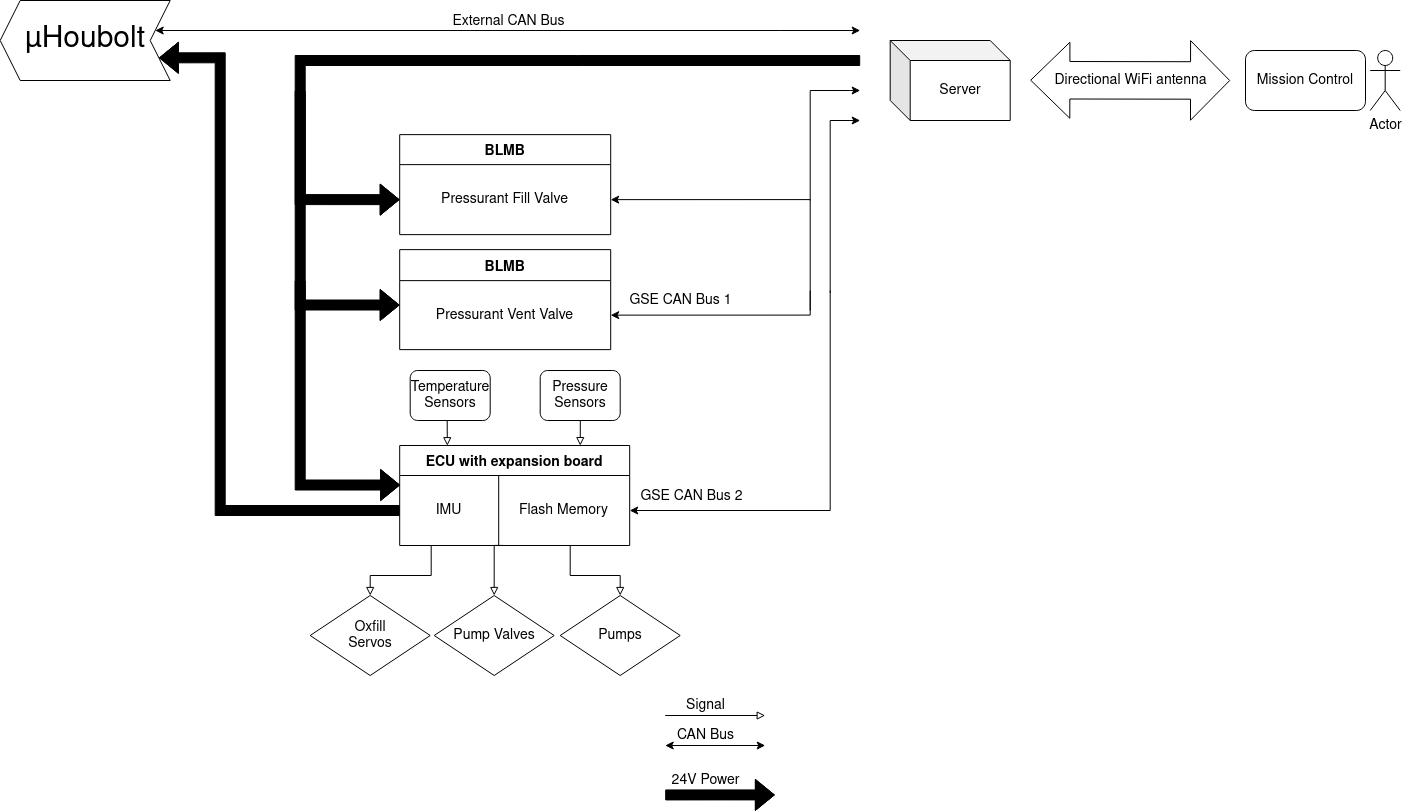
\includegraphics[width=0.9\textwidth]{GroundSystems/GSE_Blockdiagram.png}
    \caption{Subsystem Block Diagram, see \cref{fig:avi_ssbd} for the block diagram for the Avionics.}
    \label{fig:gse_ssbd}
\end{figure}

The Ground Support Equipment, including the oxidizer loading system uses a modified version of our Engine Control Unit PCB, with the outputs for the igniter being repurposed for driving the water pumps through relays. The nitrogen pressurization also takes care of the oxidizer tank pre-pressurization and utilizes two SRAD Turboservos which replaced COTS servo motors as those couldn't provide a high enough torque for actuating the valves at such high pressures, which also have their accompanying BLMB (Brushless Motor Board) PCB connected. All of these components are connected via CAN to Mission Control.

The Turboservos are SRAD servo motors which utilize a brushless DC motor connected to a servo gearbox and a rotary encoder. The control PCB is connected directly to the CAN bus and takes position commands which it translates into movement for the motor to reach the desired position which is then checked in a control loop with the rotary encoder.

The water temperature is being measured with two submersible NTC Resistors which can measure the temperature accurate to +/-\SI{0.5}{\percent}.


\subsection{Pressurant Loading System} %Johnny
%P\&ID
%Safety Analysis, Eignungsnachweis kritischer Komponenten\\ \\

\subsubsection{Overview}
The pressurant tanks inside the rocket, which are actually paintball tanks rated for \SI{310}{\bar} are pressurised to \SI{300}{\bar} through two seperate umbilicals which are fed from a nitrogen gas cylinder, as can be seen in \cref{fig:full_pnid}. Since the target pressure in the rocket's tanks is the same as the pressure inside the full nitrogen cylinder a pressure regulator is not required. Pressurisation of the rocket as well as depressurisation of the oxidiser loading system can be remotely controlled using two motorised valves.

\subsection{Umbilicals} %Johnny
\label{sec:umbilicals}

\subsubsection{Electric Connection}
The electrical umbilical is magnetically connected to a port at the top of the vehicle. During lift-off the electrical umbilical will automatically disconnect as the rocket moves along the launch rail.

\subsubsection{Fluid Umbilicals}
The fluid umbilicals are connected at three points along the side of the rocket. The upper two supply the pressurant gas while the lower one provides the oxidiser. Thus the two pressurant umbilicals consist of flexible high pressure gas line that is able to withstand the \SI{300}{\bar} inside the pressurant system. The oxidiser umbilical is a piece of flexible tubing compatible with nitrous oxide, which is reinforced with metal braiding along the outside. All three fluid umbilicals terminate in quick-disconnectors that have their counterparts on the rocket. The ends of the umbilicals are connected to the strongback that is pulled away from the rocket before the launch. In order to not apply any unnecessary torque to the rocket that could damage the rail or the railbuttons umbilical disconnectors (see \cref{fig:umbilical_disc}) are used to separate the lines from the rocket.
They are spring loaded devices that are placed over the quick-disconnects. When the strongback is pulled back it first pulls a pin (uper left) out of the umbilical disconnector that releases the spring, which presses against the airframe using a pusher plate (black). A lip at the front of the tube engages with the quick-disconnect and releases it. The strongback, which is connected to the umbilical and disconnector through the line in the lower left then pulls the device away from the rocket.

In order for this system to work reliably the oxidiser and pressurant lines first have to be depressurised.

\begin{figure}
    \centering
    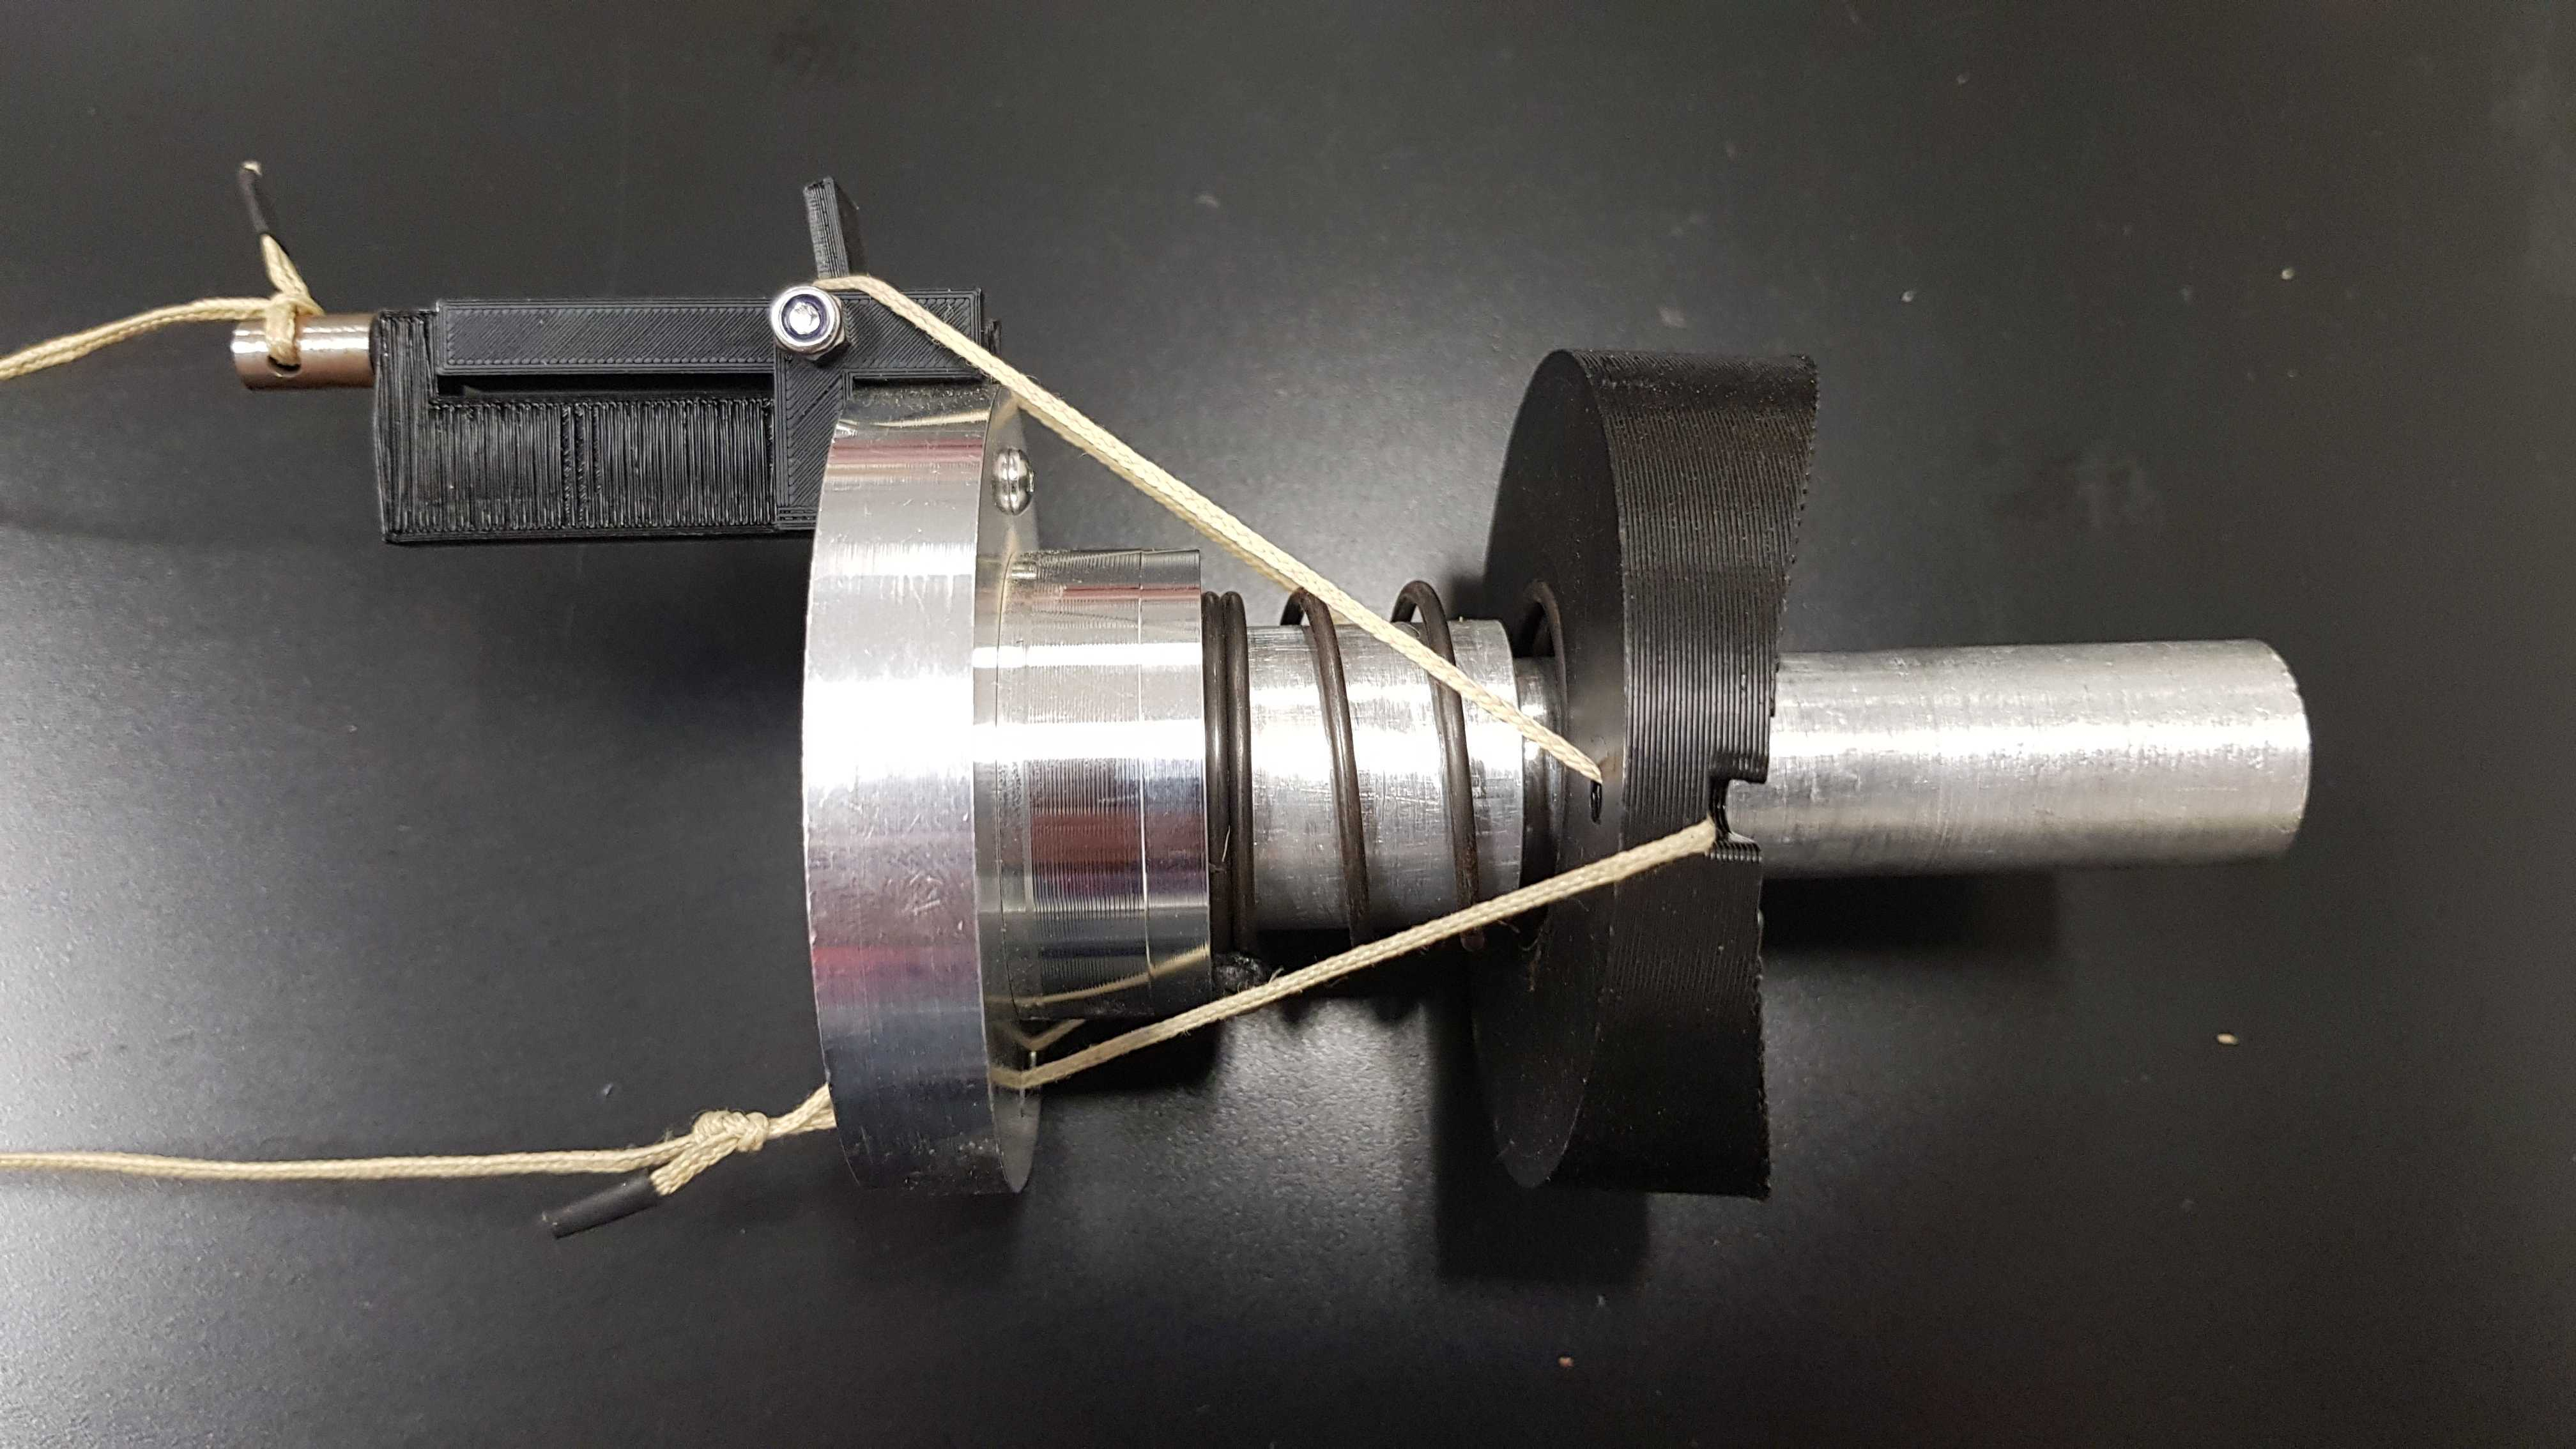
\includegraphics[width=0.9\textwidth]{GroundSystems/Umbilical_Disconnect.jpg}
    \caption{Umbilical Disconnector}
    \label{fig:umbilical_disc}
\end{figure}

\subsection{Ground Support Equipment Electronics}

This section has overlap with information on the Mission Control Software, so if interactions are unclear it is advised to read \cref{sec:software} from the appendices which covers the the software architecture.

Similarly to the rocket itself, the electronics in the launch pad are connected to the main Ubuntu Server via CAN Bus and is controlled via the same Low Level Server and Mission Control data flow as the rocket. There are three components in the GSE: A modified ECU (Engine Control Unit) board whose igniter outputs are wired to the cooling and heating pump of the oxidizer loading system, and two BLMB (Brushless Motor Board).

The launch pad is wired to the Ubuntu Server in a mobile rack with a CAN cable and the server rack is connected to the Mission Control with a directed radio link. In the server rack, connected directly to the server via LAN, a Raspberry Pi single board computer with a LoRa shield is used for the \SI{433}{\mega\hertz} radio connection to the rocket during flight.

The entire GSE is powered using mobile power generators and during launch preparations the electronics umbilical also provides power to the rocket, keeping the internal batteries charged until automatic disconnect at lift-off.

\newpage

\chapter{Concept of Operations}
\label{chap:conops}

\section{Rocket lifecycle during EuRoC}
\begin{enumerate}
    \item Rocket gets presented at the exhibition.
    \item On the day before the launch, the rocket gets assembled, the recovery section prepared and the electronics checked.
    \item On the launch day we bring the rocket to the launch site and start going through the launch day checklists.
    \item After landing we recover the rocket and bring it back to the launch.
    \item After inspection of the rocket, we bring it back to the exhibition area.
\end{enumerate}

\section{Launch Procedure}

\subsection{Vehicle Assembly}
\begin{enumerate}
\item Pulling the RBF.
\item Testing electronics - running test and launch sequence.
\item Inserting the RBF halfway.
\item Starting fuel loading process (see chapter ref \ref{Fuel Loading}).
\item Checking the water state (cooling and heating cycle).
\item Checking that the igniter electronics are deactivated.
\item Installing the igniters.
\item Mounting the Fincan to the body tube.
\item Vacating the launch area.
\end{enumerate}

\subsection{Mission Control Setup}
\begin{enumerate}
\item Connecting directed radio link and Raspberry Pi with LoRa shield to server.
\item Powering on server, Mission Control PC and monitors.
\item Connecting Mission Control PC to server via LAN.
\item Opening Mission Control Web-Application on Web-Browser.
\end{enumerate}

\subsection{Launch Pad Setup}
\begin{enumerate}
\item Mounting flame diverter.
\item Connecting GSE to directed radio link.
\item Filling water reservoirs.
\item Flipping, installing and sealing oxidizer bottle inside temperature exchange mantle.
\item From now on continuously check and add ice to cold water reservoir.
\item Installing pressurant bottle.
\item Sliding rocket onto launch rail.
\item Mounting T-nut underneath lower rail button.
\item Securing and closing holddown above lower rail button.
\item Connecting oxidizer, pressurant and electrical umbilicals.
\item Pulling RBF pin halfway to power on avionics.
\item Checking sensors and actuators, verifying movement and calibration, via Mission Control.
\end{enumerate}

\subsection{Fuel Loading} \label{Fuel Loading}
\begin{enumerate}
\item Closing fuel main valve.
\item Mounting the tyre fill adapter connected to the syringe filled with ethanol to the fuel inlet section to open the check valve completely.
\item Applying force to the syringe to fill the tank with a precise amount of fuel and enabling the ullage gas to exit the tank through the small bleed orifice.
\item Removing the syringe from the rocket after filling.
\item Covering the rocket’s fuel inlet section.
\end{enumerate}

\subsection{Final Pad preps}
\begin{enumerate}
\item Opening oxidizer bottle and checking for leaks.
\item Opening pressurant bottle and checking for leaks.
\item Staring pad cameras.
\item Pulling RBF pin to connect power to ignition circuitry.
\end{enumerate}

From this point onwards the rest of the preparations until launch can be done completely remotely. 

\subsection{Oxidizer Loading}
\label{sec:oxidizer_loading}
Pressure and temperature data is closely monitored throughout the whole process.
\begin{enumerate}
\item Closing oxidizer main valve.
\item Activating and setting the vent valve pressure regulation to 30 bar.
\item Closing pressurant vent valve.
\item Opening pressurant tanking valve for filling pressurant until vent valve gets activated. Then closing pressurant tanking valve.
\item Closing oxidizer vent valve.
\item Opening oxidizer fill valve to start the oxidizer loading.
\item Activating the heating cycle in the oxidizer bottle.
\item Quickly closing oxidizer fill valve when plume (venting liquid oxidizer) is visible.
\item Deactivating the heating cycle/activating the cooling cycle in the oxidizer bottle.
\item Opening oxidizer fill valve again after a stabilization of the venting frequency.
\item Quickly closing oxidizer fill valve when plume is visible. 
\item Opening oxidizer vent valve.
\end{enumerate}

\subsection{Pressurant Loading}
\label{sec:pressurant_loading}
\begin{enumerate}
\item Deactivating vent valve pressure regulation.
\item Opening pressurant tanking valve.
\item Waiting for stable pressurization.
\item Closing pressurant tanking valve.
\item Opening pressurant vent valve.
\item Activating umbilical retract of pressurant and oxidizer tanking lines and verifying clean separation.
\end{enumerate}

\subsection{Internal Countdown and Launch}
\begin{enumerate}
\item Activating the rockets internal control via Mission Control after Go/NoGo.
\item The rocket does a continuity check on the igniters, if continuity is given,  start internal countdown.
\item The rocket checks for proper engine performance after ignition. This is measured by a proxy measurement of combustion chamber pressure. The threshold is set beforehand by Mission Control and is usually set to around \SI{10}{\bar}.
\item If proper engine performance is detected by the rocket, it sends a signal to the Launch Pad to release the holddown.
\item Lift-Off is achieved once the electrical umbilical that is magnetically held in place gets disconnected by the rocket moving out of reach.
\end{enumerate}

Until lift-off there is still a possibility for manual abort from Mission Control. Beginning with lift-off and the electrical umbilical disconnecting the rocket is monitoring itself and no manual abort is possible. The rocket is now in powered ascent phase.

The entire engine burn duration is \SI{8}{\second} long, after which the main valves are closed and we have achieved MECO (Main Engine Cut Off). Since the propellant tanks are sized for this \SI{8}{\second} burn duration, alternatively the engine could also just be left open to run out of propellant (which should happen roughly \SI{8.8}{\second} after ignition). This approach has the advantage of not needing to open the main valves again for complete depressurization.

From then on, the rocket is in unpowered ascent until apogee is detected and recovery is triggered.

\subsection{Recovery}
\begin{enumerate}
\item Opening vent valve pressure regulation.
\item Closing vent valve pressure regulation when the tanks are fully depressurized.
\item Opening fuel main valve for remaining fuel unloading.
\item Separation of the nose cone from the body tube at apogee.
\item Drogue chute release at apogee.
\item Main chute release \SI{250}{\meter} altitude. Backup Altimax triggers at \SI{200}{\meter}.
\item Recovering the rocket after landing.
\end{enumerate}

\subsection{GSE Safing}
\begin{enumerate}
\item Stopping all cameras.
\item Closing the oxidizer bottle.
\item Closing the pressurant bottle.
\item Vacating the pad area.
\item Opening oxidizer fill valve.
\item Opening pressurant tanking valve.
\item Checking all pressure data to verify a full depressurization of the system.
\item Announcing "safe state".
\end{enumerate}


\newpage

\chapter{Conclusion and Outlook}
\label{sec:conclusion}

Our motivation back when starting the liquid propulsion project within the Space Team was both to be able to work on extremely cool technologies and learn a lot while trying to develop our own rocket engines, as well as pushing the boundaries of what is thought to be possible for a student team to achieve. Throughout the over three years since the first endeavours in liquid engines, we have learned so much about the technology and its limits, developed extensive testing infrastructure and built a staggering amount of prototypes.

The project we have actively worked on has slowly morphed from the gigantic Houbolt rocket to the small scale technology demonstrator \uH and we also branched out into sub-projects like GATE, a Houbolt-sized engine concept to go along with our large engine test stand - but the main goal has stayed the same: pushing boundaries. We have managed to build and operate the largest rocket engine in Austria, built a reliable small scale engine to be used in \uH and now have a rocket to demonstrate these capabilities.

However, all of this would be in vain if all this progress gets lost once the project concludes. No one can be part of such an ambitious project during their free time forever and as such the probably most important part of the project is the final documentation of it. Once all is said and done and the pressure of internal goals and milestones has passed, we plan to clean up and organize our project files; from CAD models to PCB designs, software infrastructure and engine designs. When that is done it is planned to release everything needed to make a "\uH 2.0" to open source - but that's not all! \uH has been a tremendous undertaking, but we do have plans for the future internally as well: Having now proven we can build a reliable engine, it's time to do more interesting things with it than just aimlessly shooting a rocket into the sky. The next twinkle in our eyes is $\mu$Houverer, a craft that can propulsively take off and land powered by a bi-liquid rocket engine.

\newpage

\chapter{Appendices}
\label{sec:appendices}

\section{System Data}

\begin{table}[h]
\centering
\begin{tabular}{|l|l|}
\hline
\textbf{Mass (Dry)}                     & \SI{8950}{\gram} \\ \hline
\textbf{Mass (Wet)}                     & \SI{12040}{\gram} \\ \hline
\textbf{Tank Volume (Fuel)}             & \SI{900}{\milli\liter} \\ \hline
\textbf{Tank Volume (Ox)}               & \SI{2400}{\milli\liter} \\ \hline
\textbf{Length}                         & \SI{2100}{\milli\meter} \\ \hline
\textbf{Diameter (Body)}                & \SI{123}{\milli\meter} \\ \hline
\textbf{Diameter (Fins)}                & \SI{383}{\milli\meter} \\ \hline
\textbf{Pressurant Pressure}            & \SI{300}{\bar} \\ \hline
\textbf{Oxidizer Pressure}              & \SI{40}{\bar} \\ \hline
\textbf{Fuel Pressure}                  & \SI{30}{\bar} \\ \hline
\textbf{Pressurant Pressure}            & \SI{300}{\bar} \\ \hline
\textbf{Nominal Thrust}                 & \SI{600}{\newton} \\ \hline
\textbf{Combustion Chamber Pressure}    & \SI{15}{\bar} \\ \hline
\textbf{Burn Duration}                  & \SI{8}{\second} \\ \hline
\textbf{Max Speed}                      & \SI{307}{\meter\per\second} (Mach 0.92) \\ \hline
\textbf{Apogee}                         & \SI{3}{\kilo\meter} \\ \hline
\textbf{Descent Rate (Drogue)}          & \SI{39}{\meter\per\second} \\ \hline
\textbf{Descent Rate (Main)}            & \SI{7.6}{\meter\per\second} \\ \hline
\textbf{Altitude Main Chute Deployment} & Main Altimax: \SI{250}{\meter}, Backup Altimax: \SI{200}{\meter} \\ \hline
\textbf{RF (LoRa) Frequency}            & \SI{433}{\mega\hertz} \\ \hline
\end{tabular}
\caption{General System Data}
\label{tab:system_data}
\end{table}

\section{Detailed Test Reports}

\subsection{Ground Test Demonstration of Recovery System}

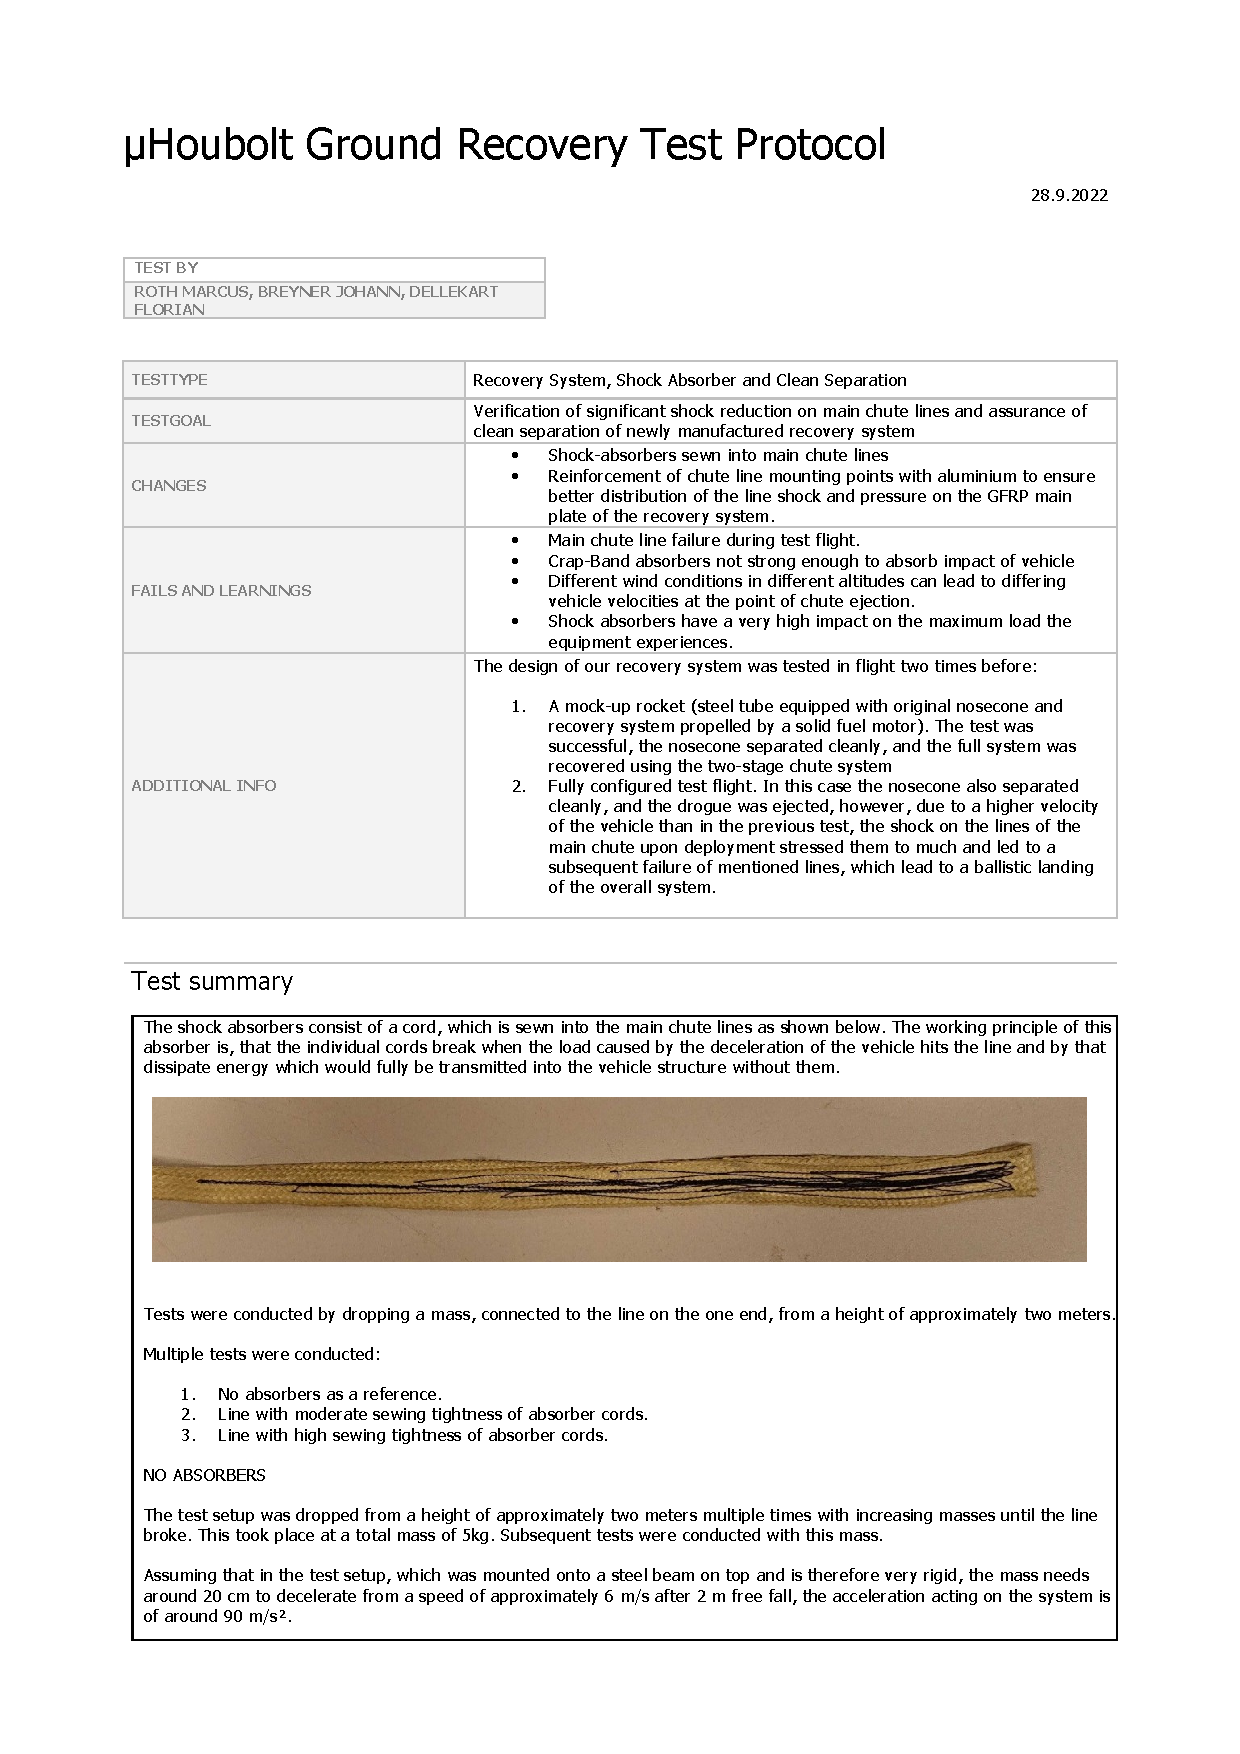
\includepdf[pages={1-4}]{Appendices/uHouboltRecoveryTestProtocol.pdf}

\newpage

\subsection{Flight Test Demonstration of Recovery System}

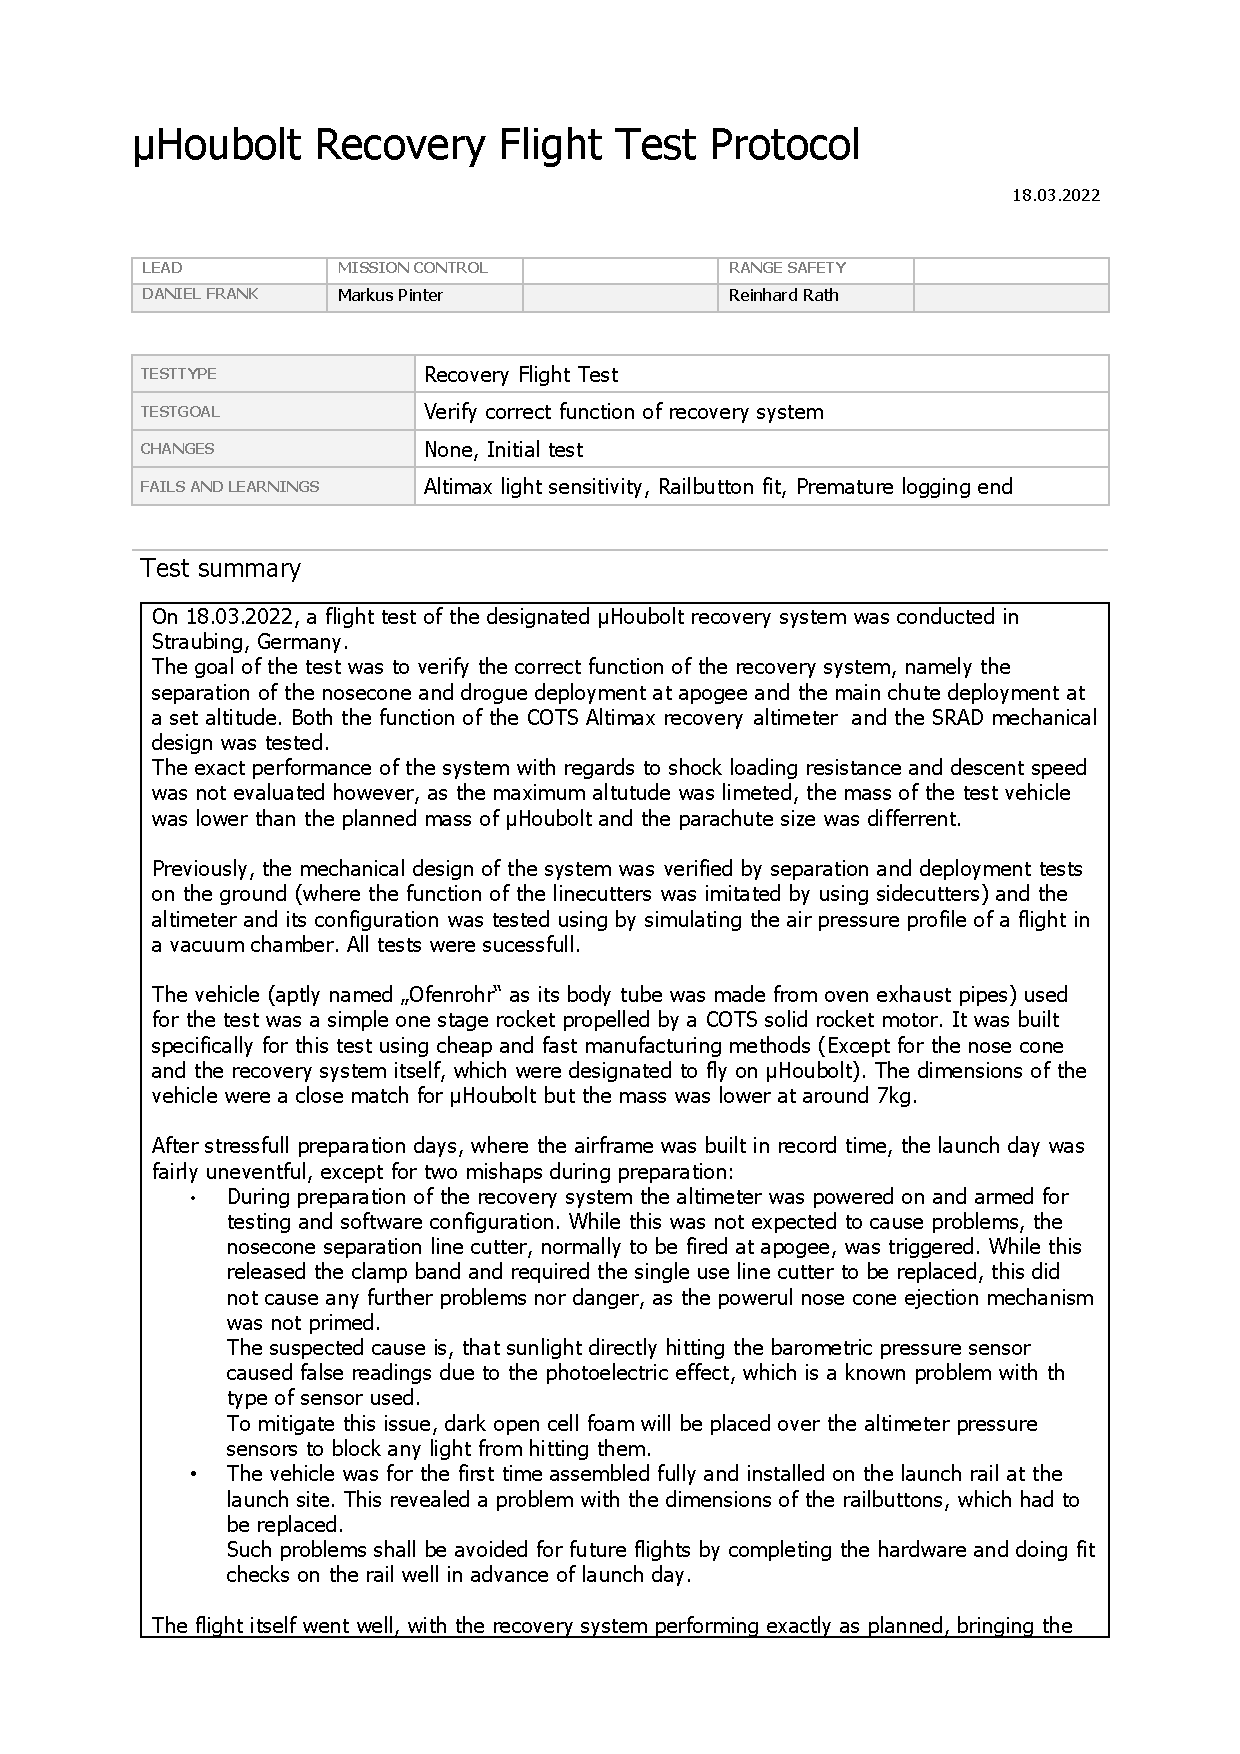
\includepdf[pages=-]{Appendices/uHoubolt_Recovery_Flight_Test_signed.pdf}

\subsection{Static Hot-Fire}

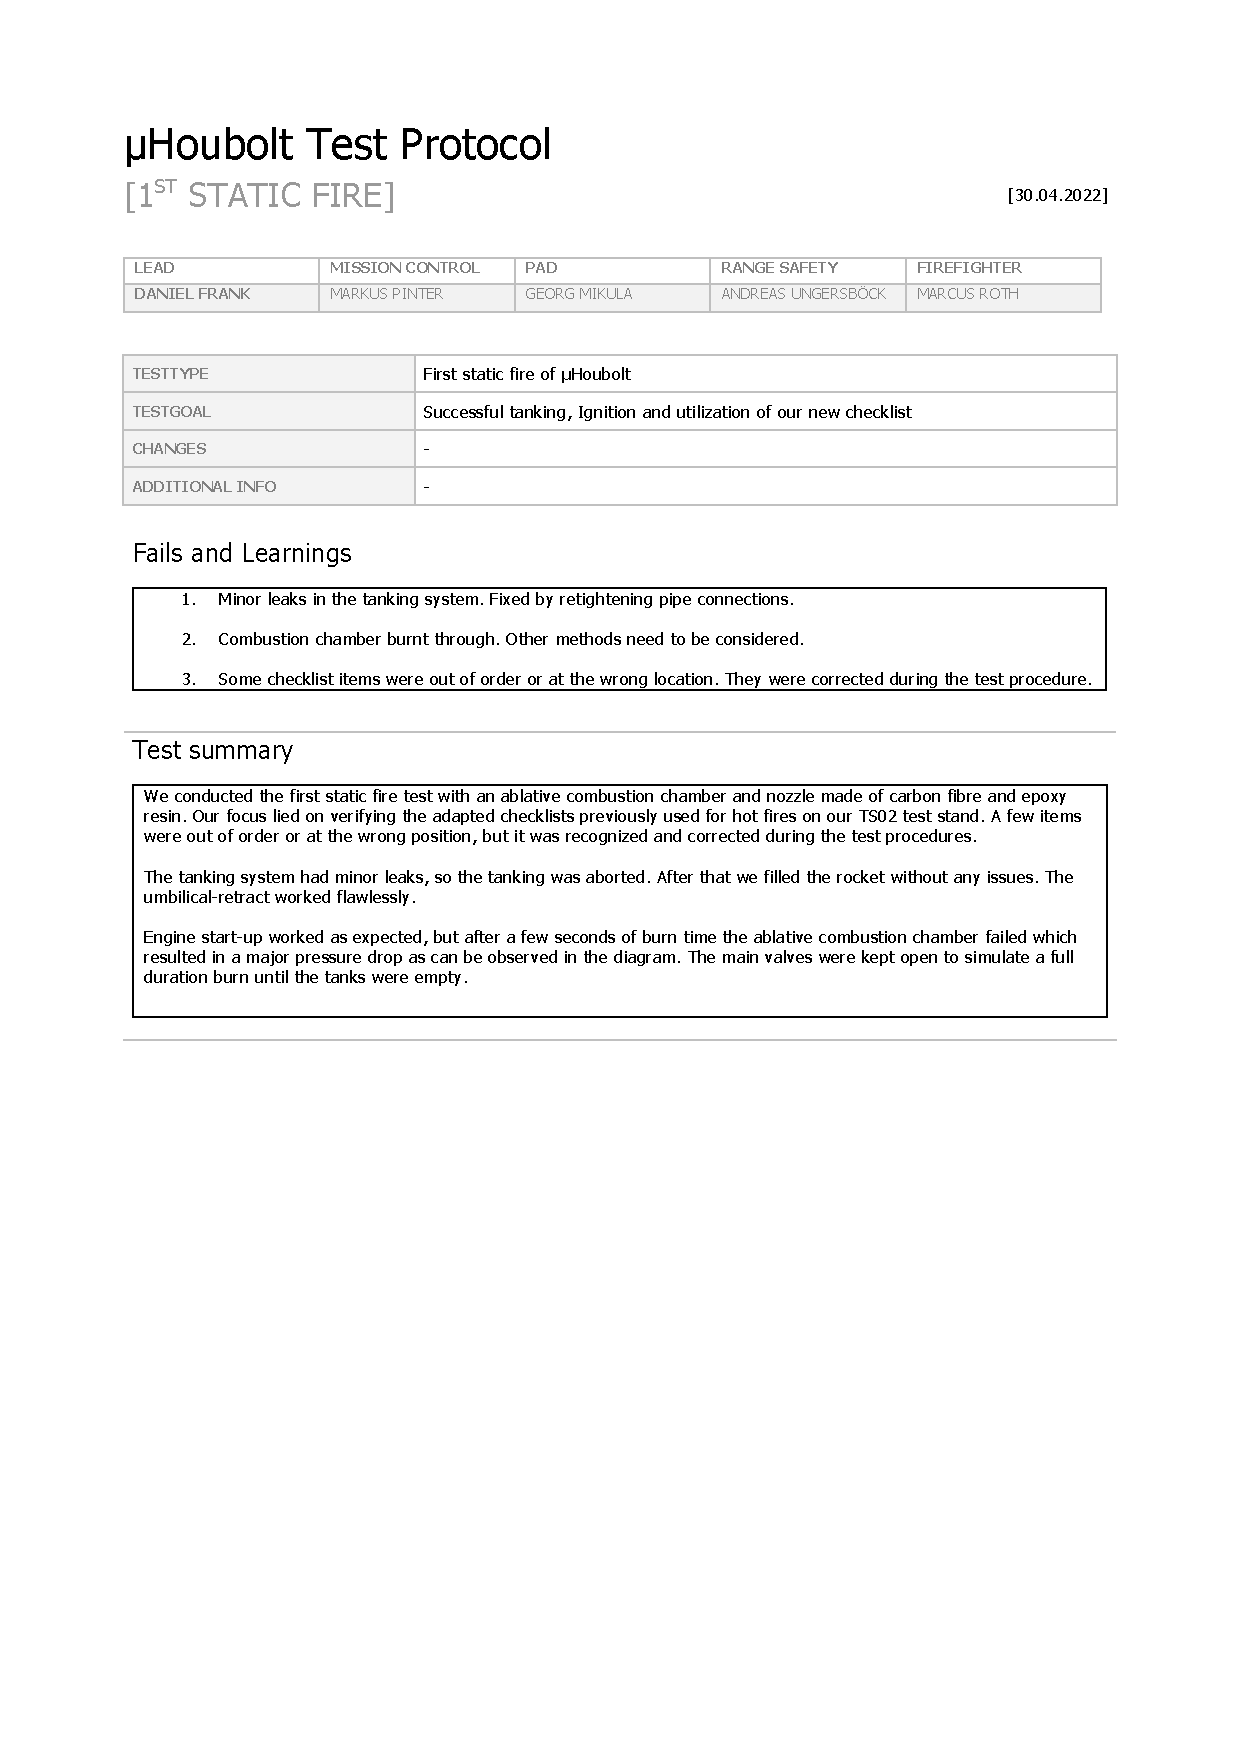
\includepdf[pages=-]{Appendices/uHoubolt_static_fire_220430_protocol.pdf}
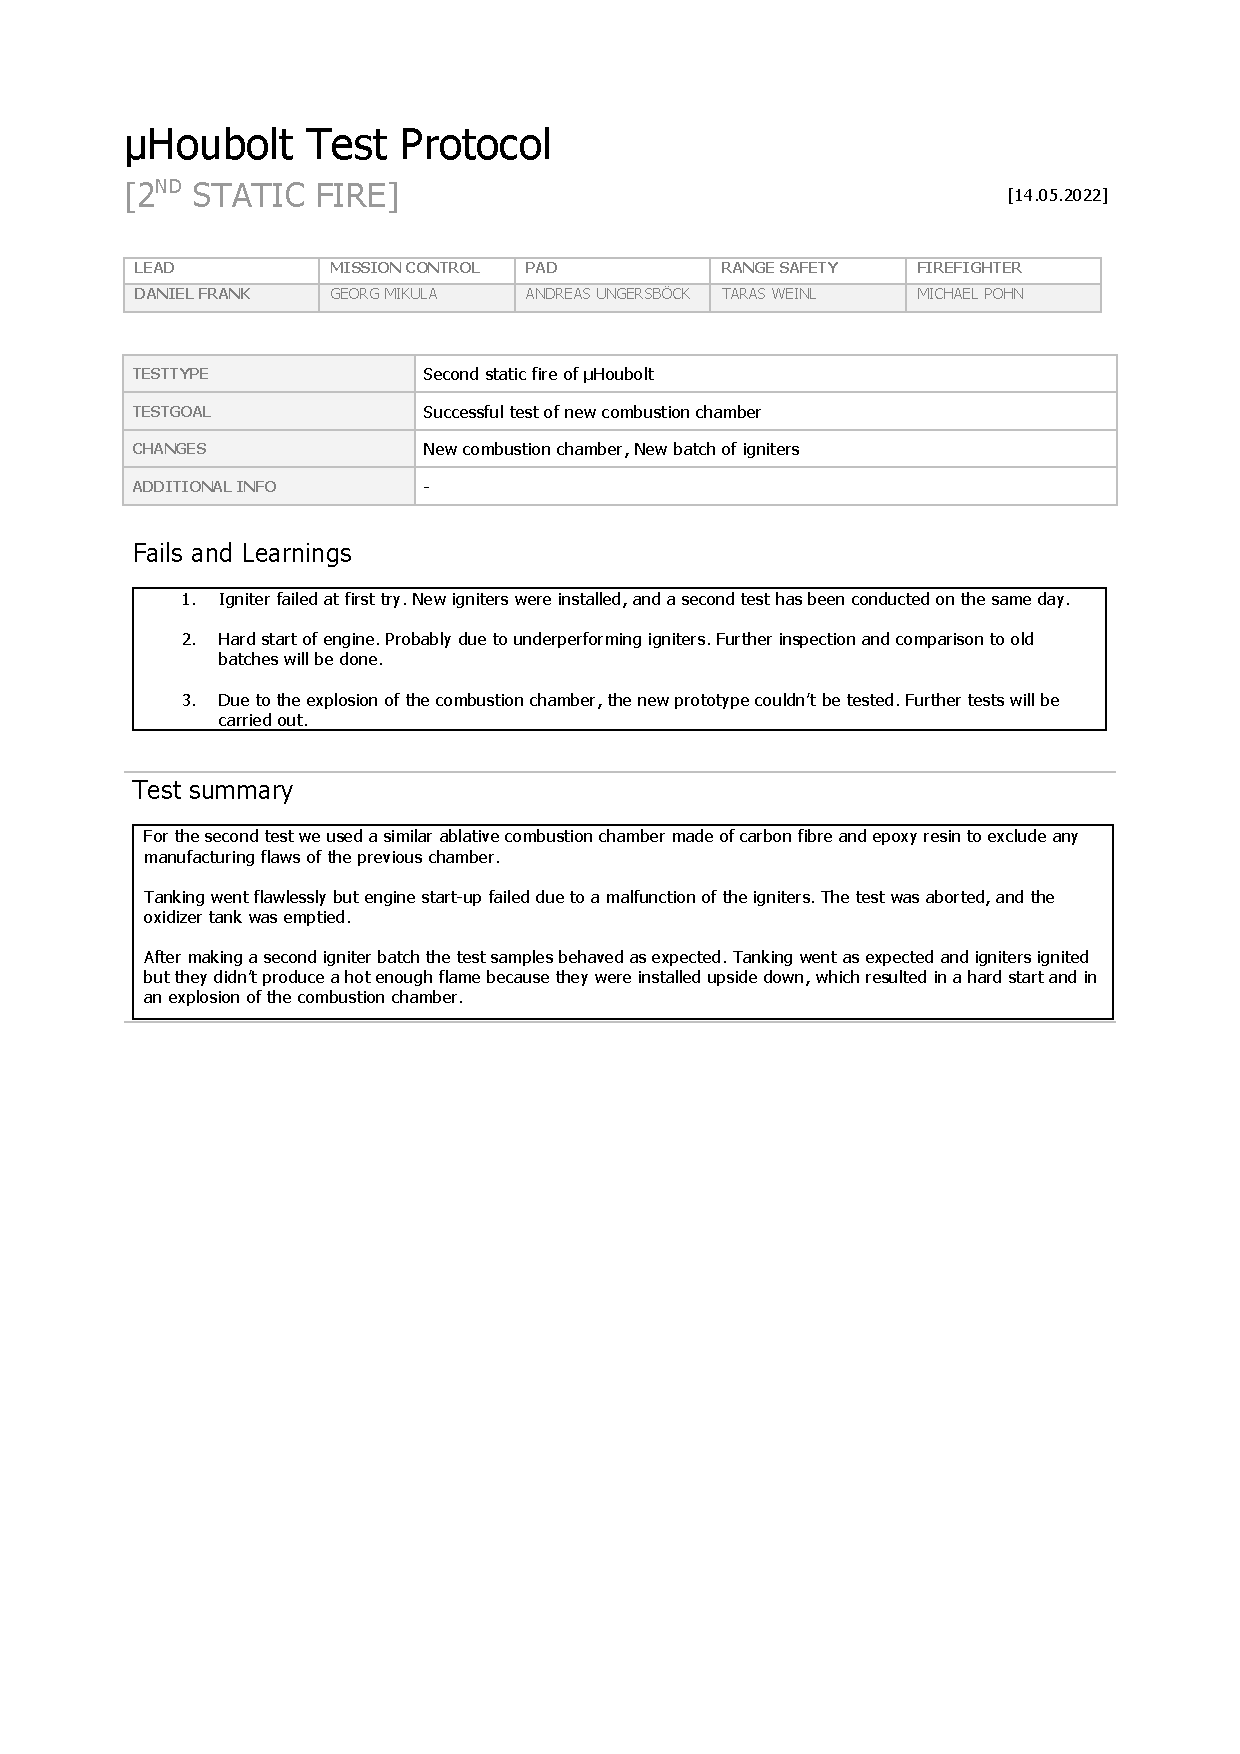
\includepdf[pages=-]{Appendices/uHoubolt_static_fire_220514_protocol.pdf}
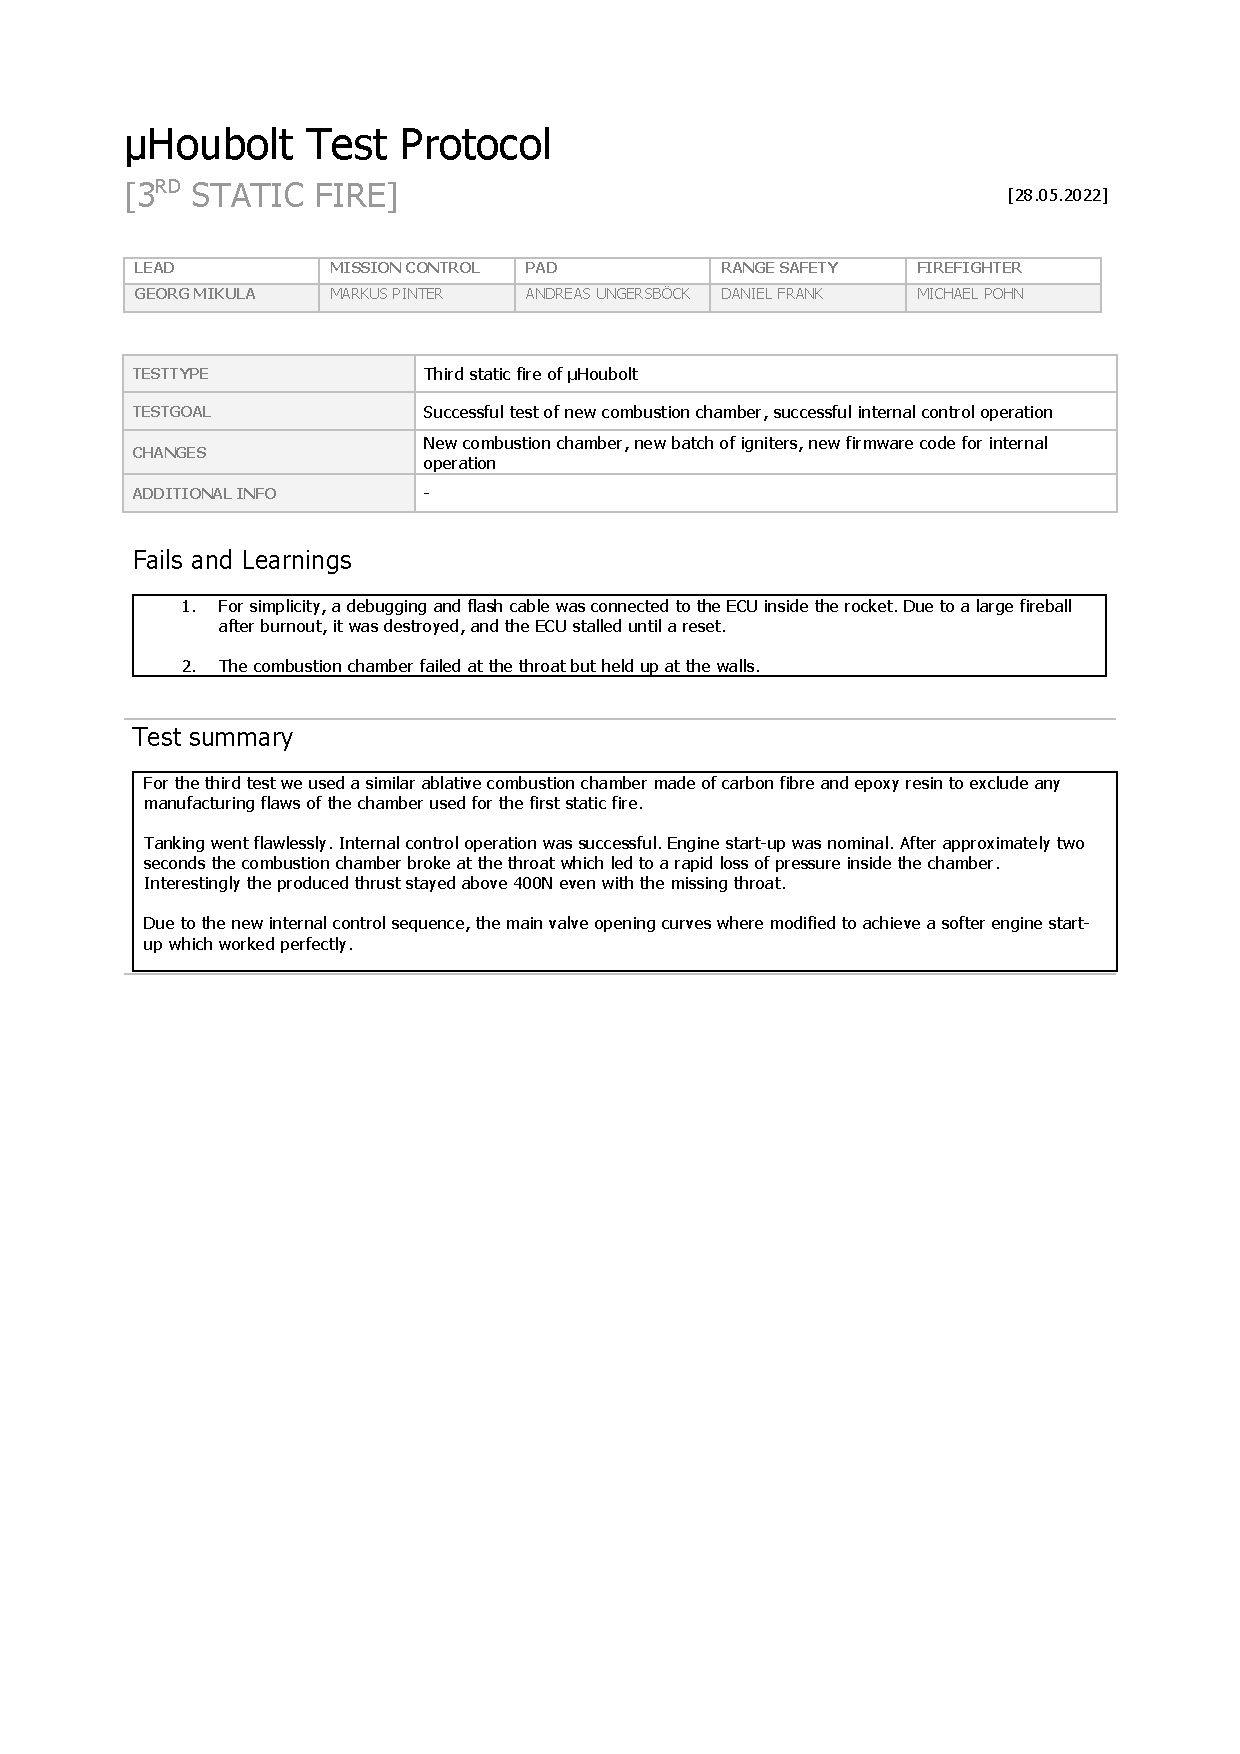
\includepdf[pages=-]{Appendices/uHoubolt_static_fire_220528_protocol.pdf}
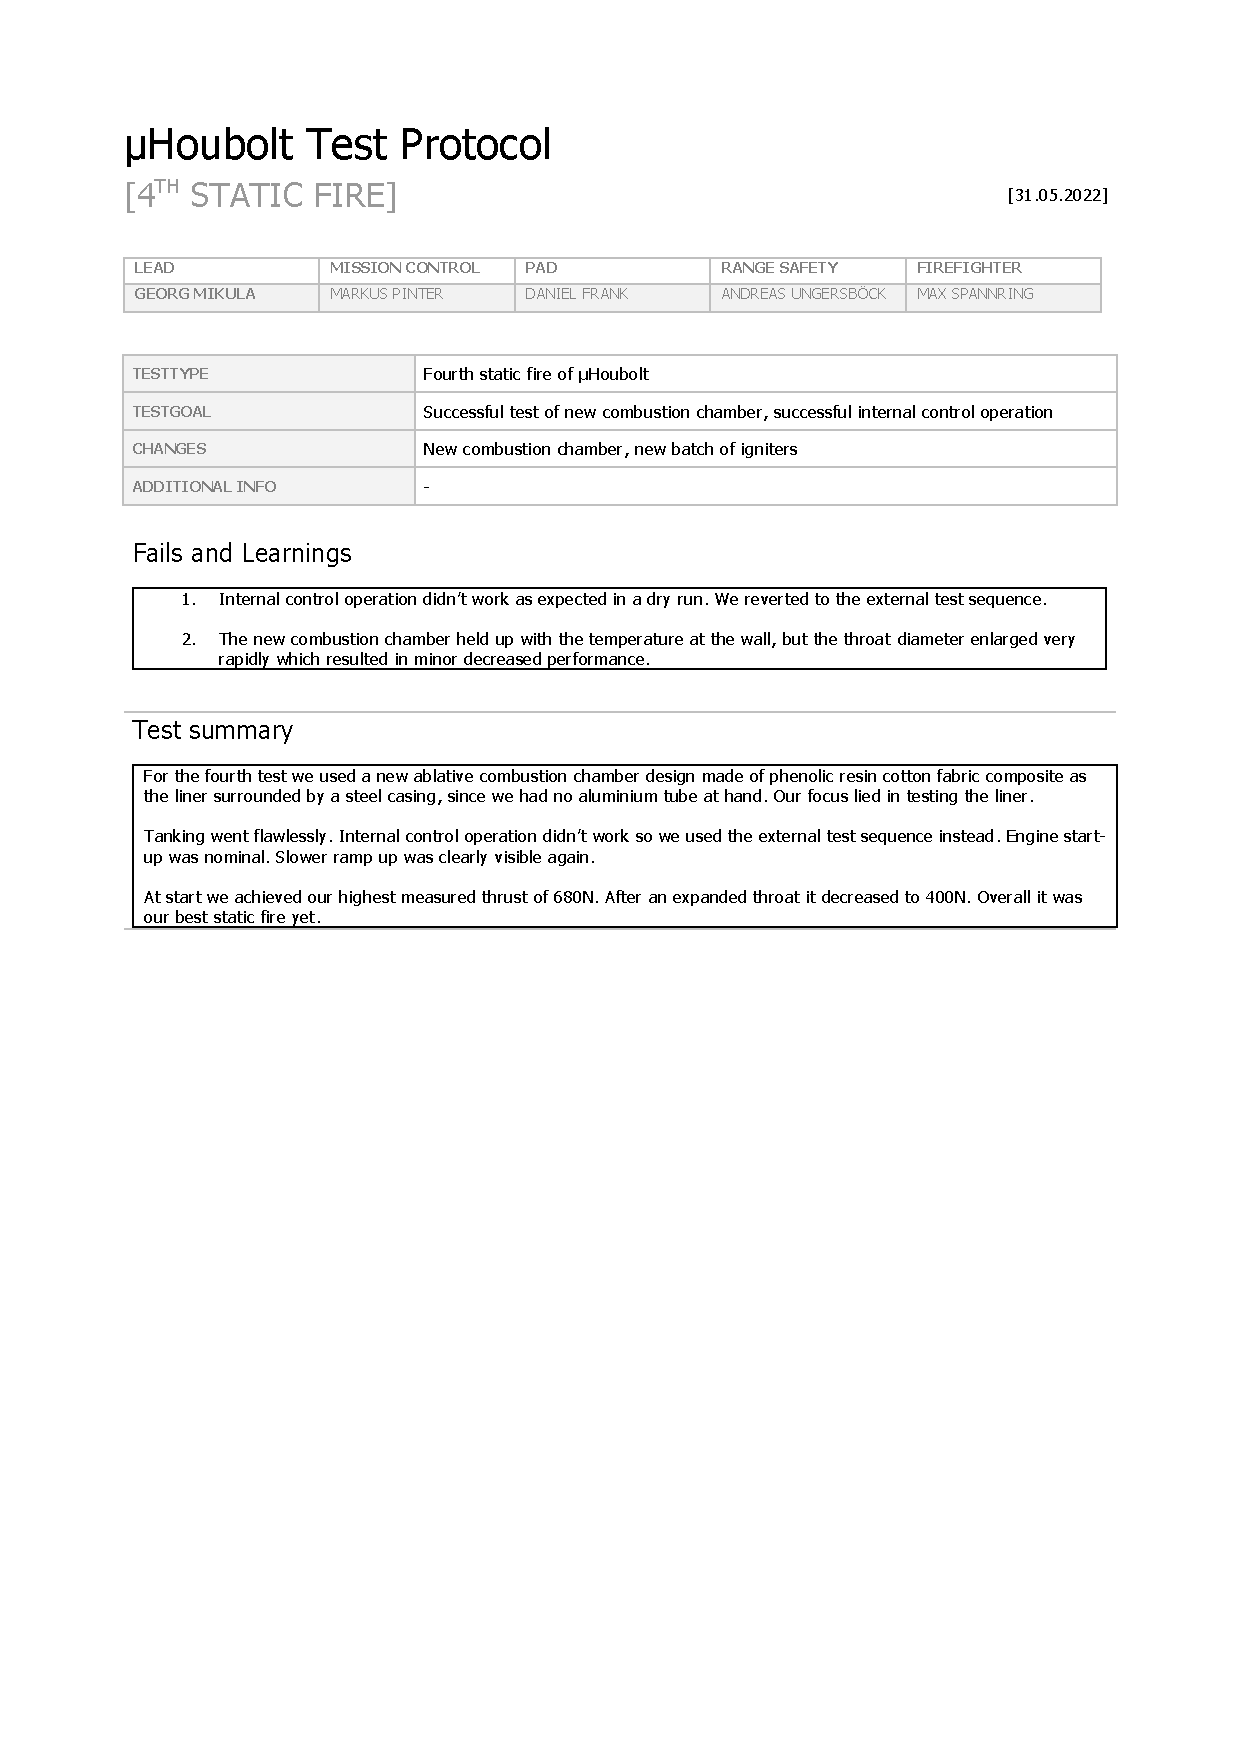
\includepdf[pages=-]{Appendices/uHoubolt_static_fire_220531_protocol.pdf}
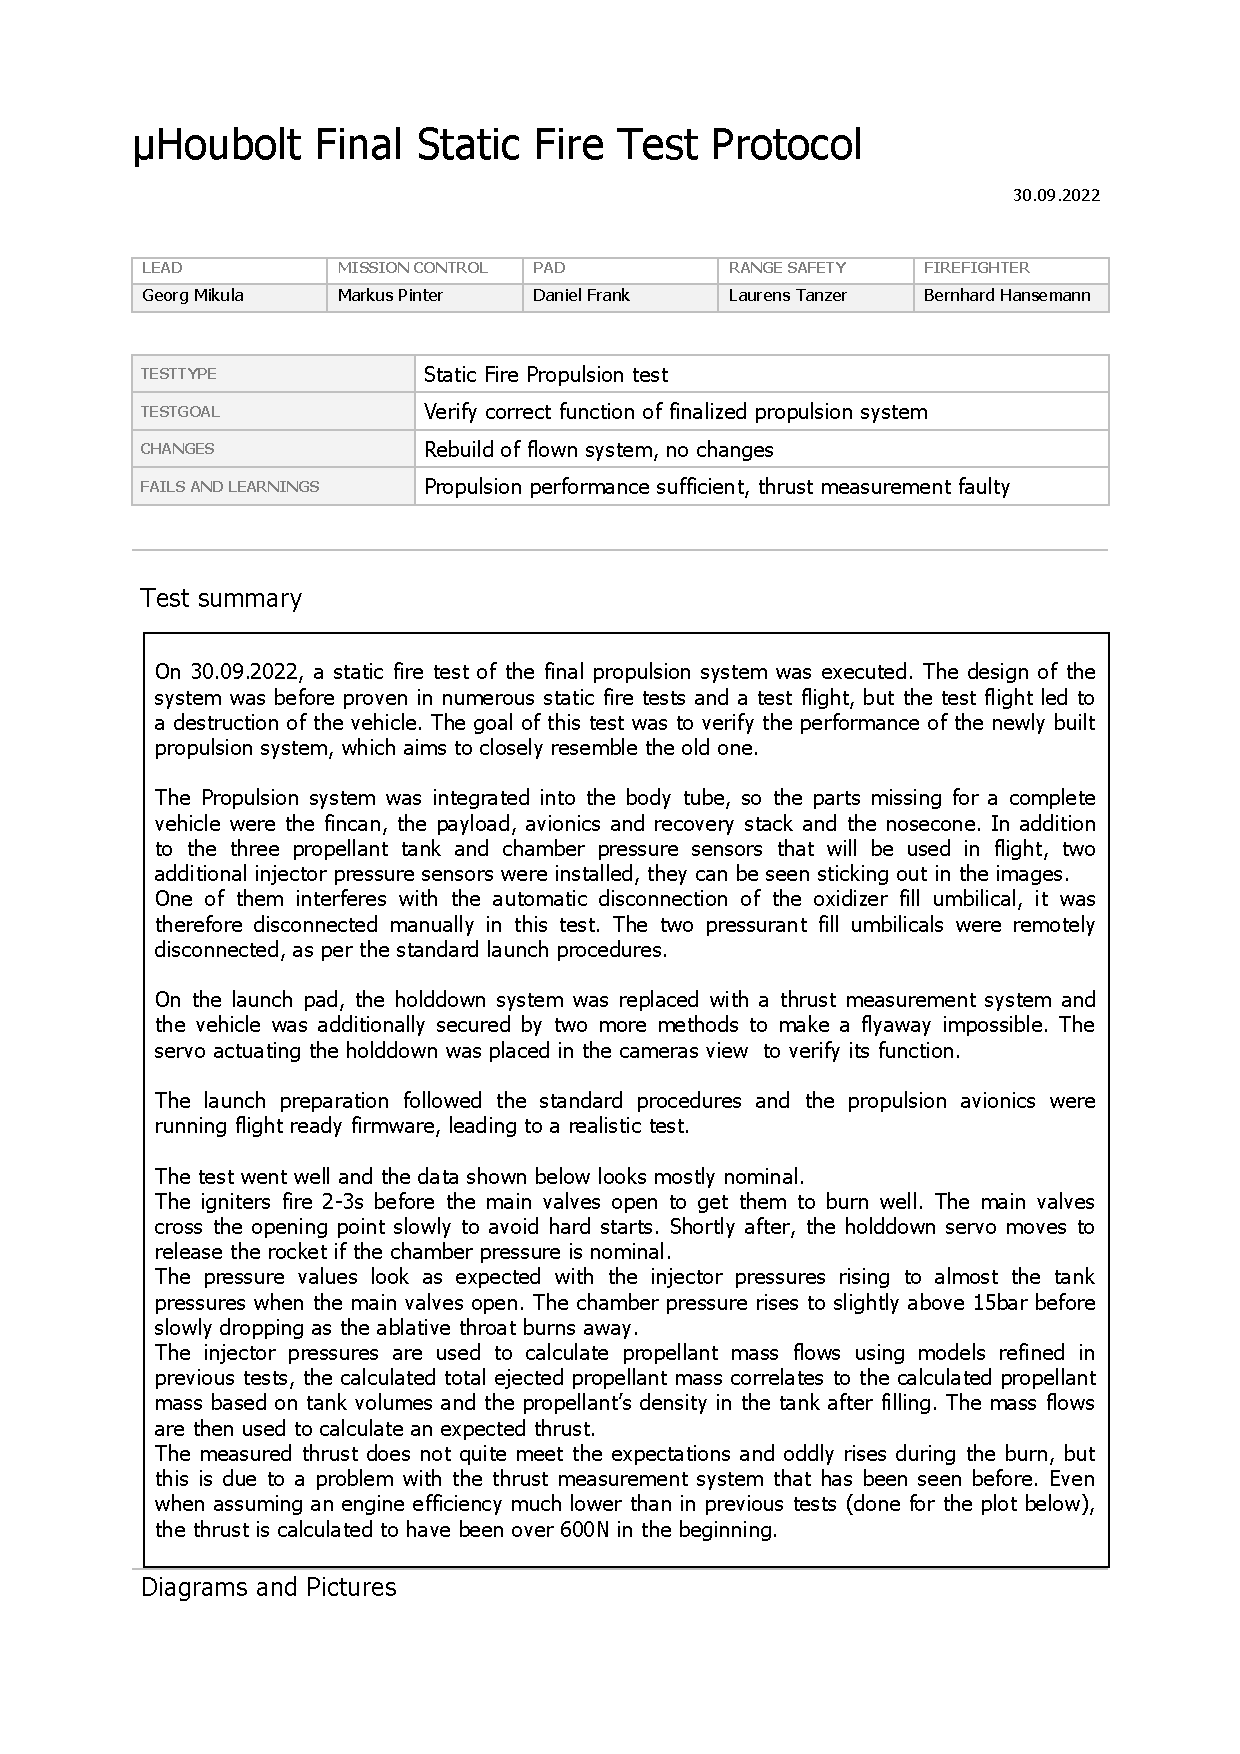
\includepdf[pages=-]{Appendices/uHoubolt_Static_Fire_Test_Protocol.pdf}

\subsection{Liquid Propellant loading and off-loading}

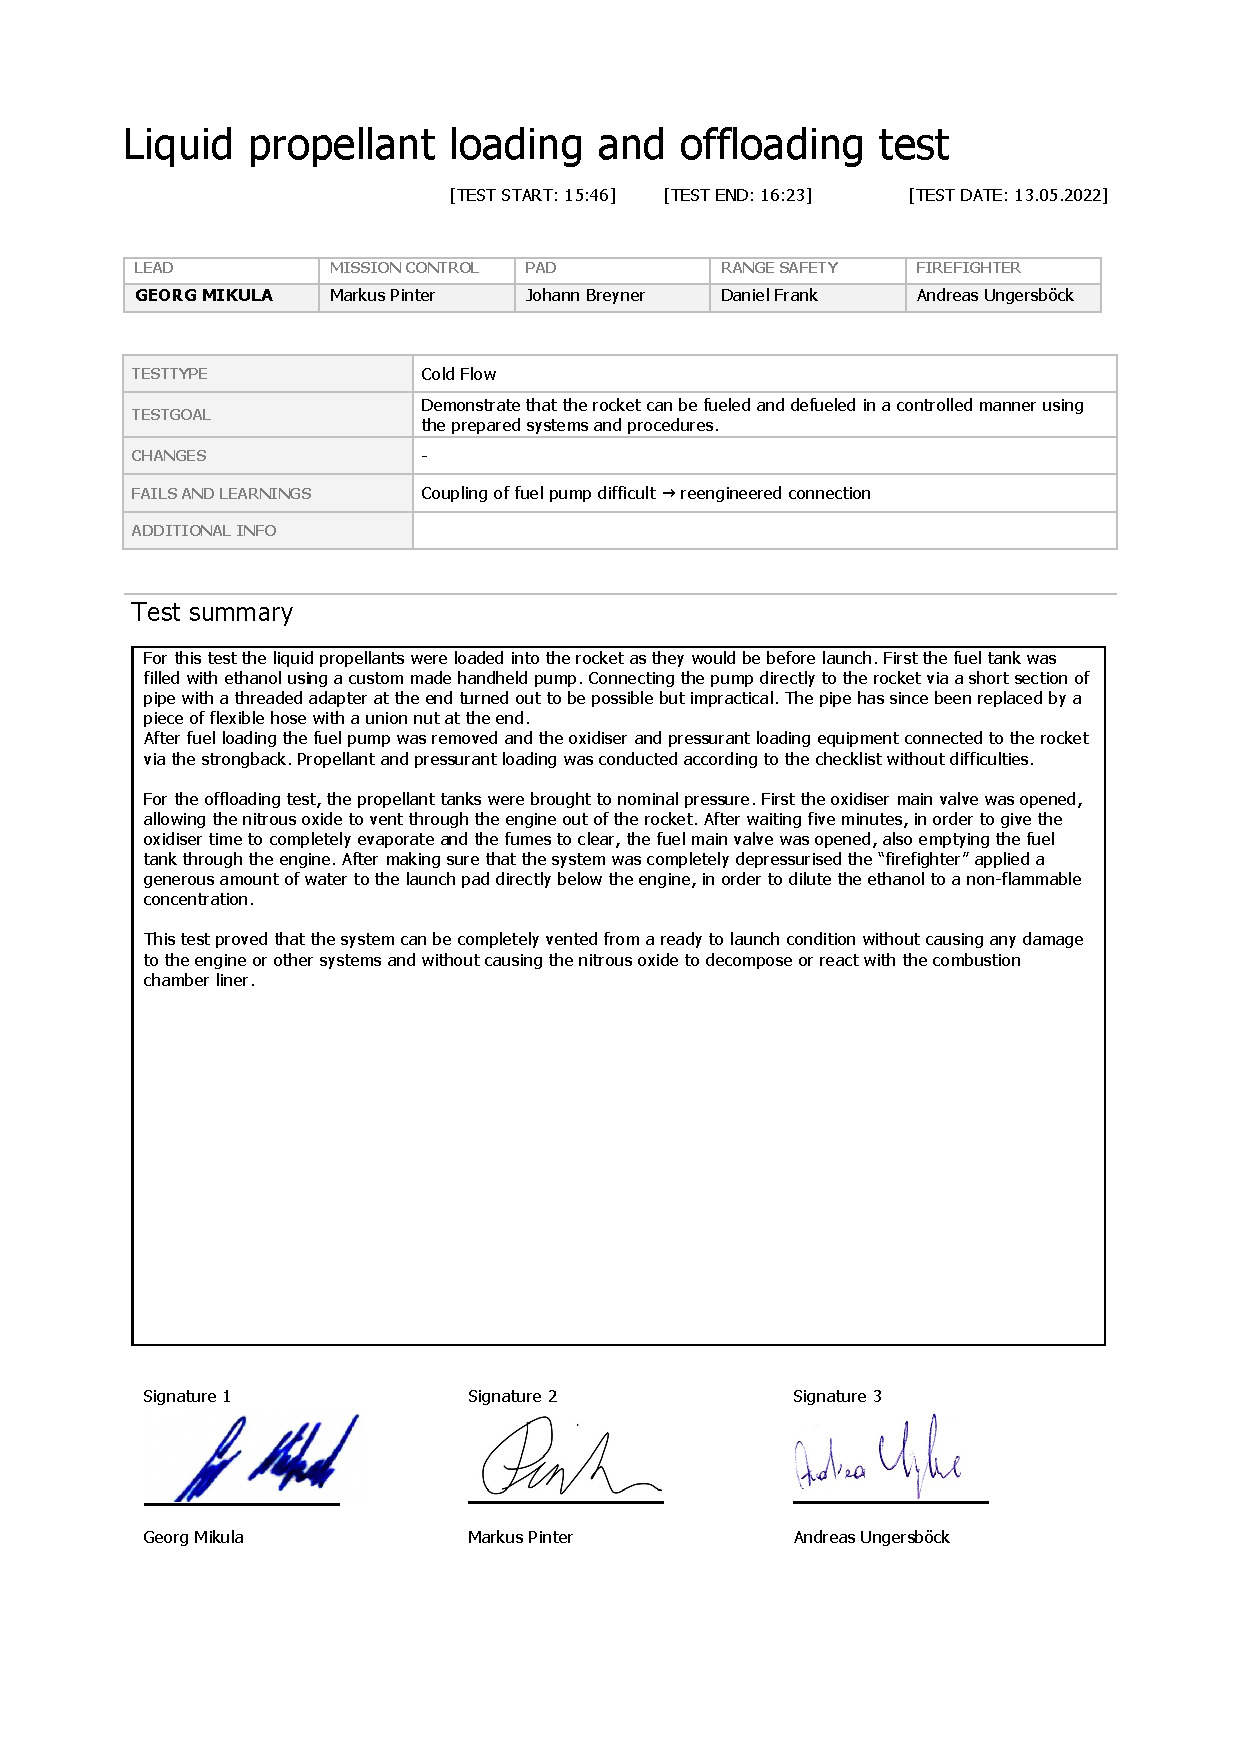
\includepdf[pages=-]{Appendices/uHoubolt_Loading_Offloading_signed.pdf}

\subsection{Combustion Chamber Pressure}

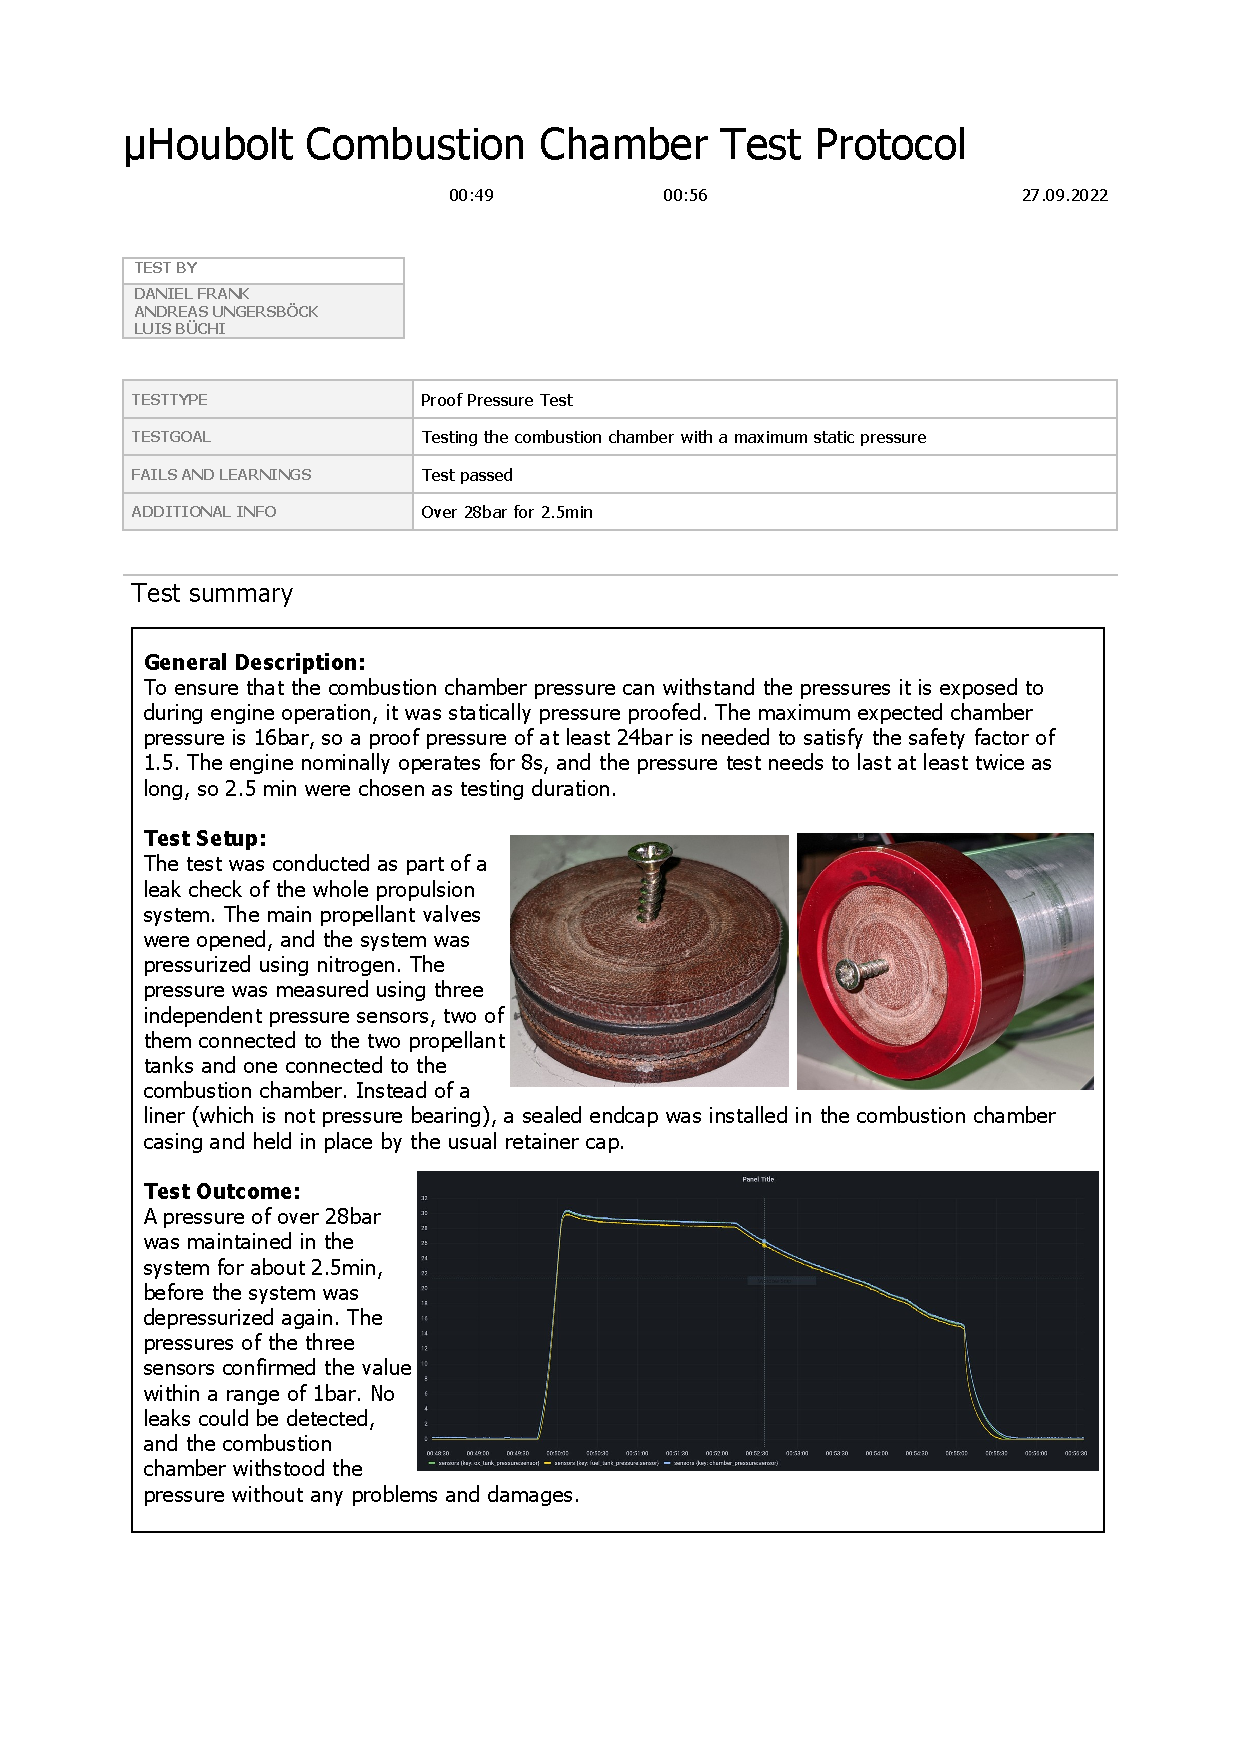
\includepdf[pages=-]{Appendices/uHoubolt_Combustion_Chamber_Test_Protocol.pdf}

\newpage

\subsection{Proof Pressure Testing Pressure Vessels}\label{sec:app_proof_pressure_testing}

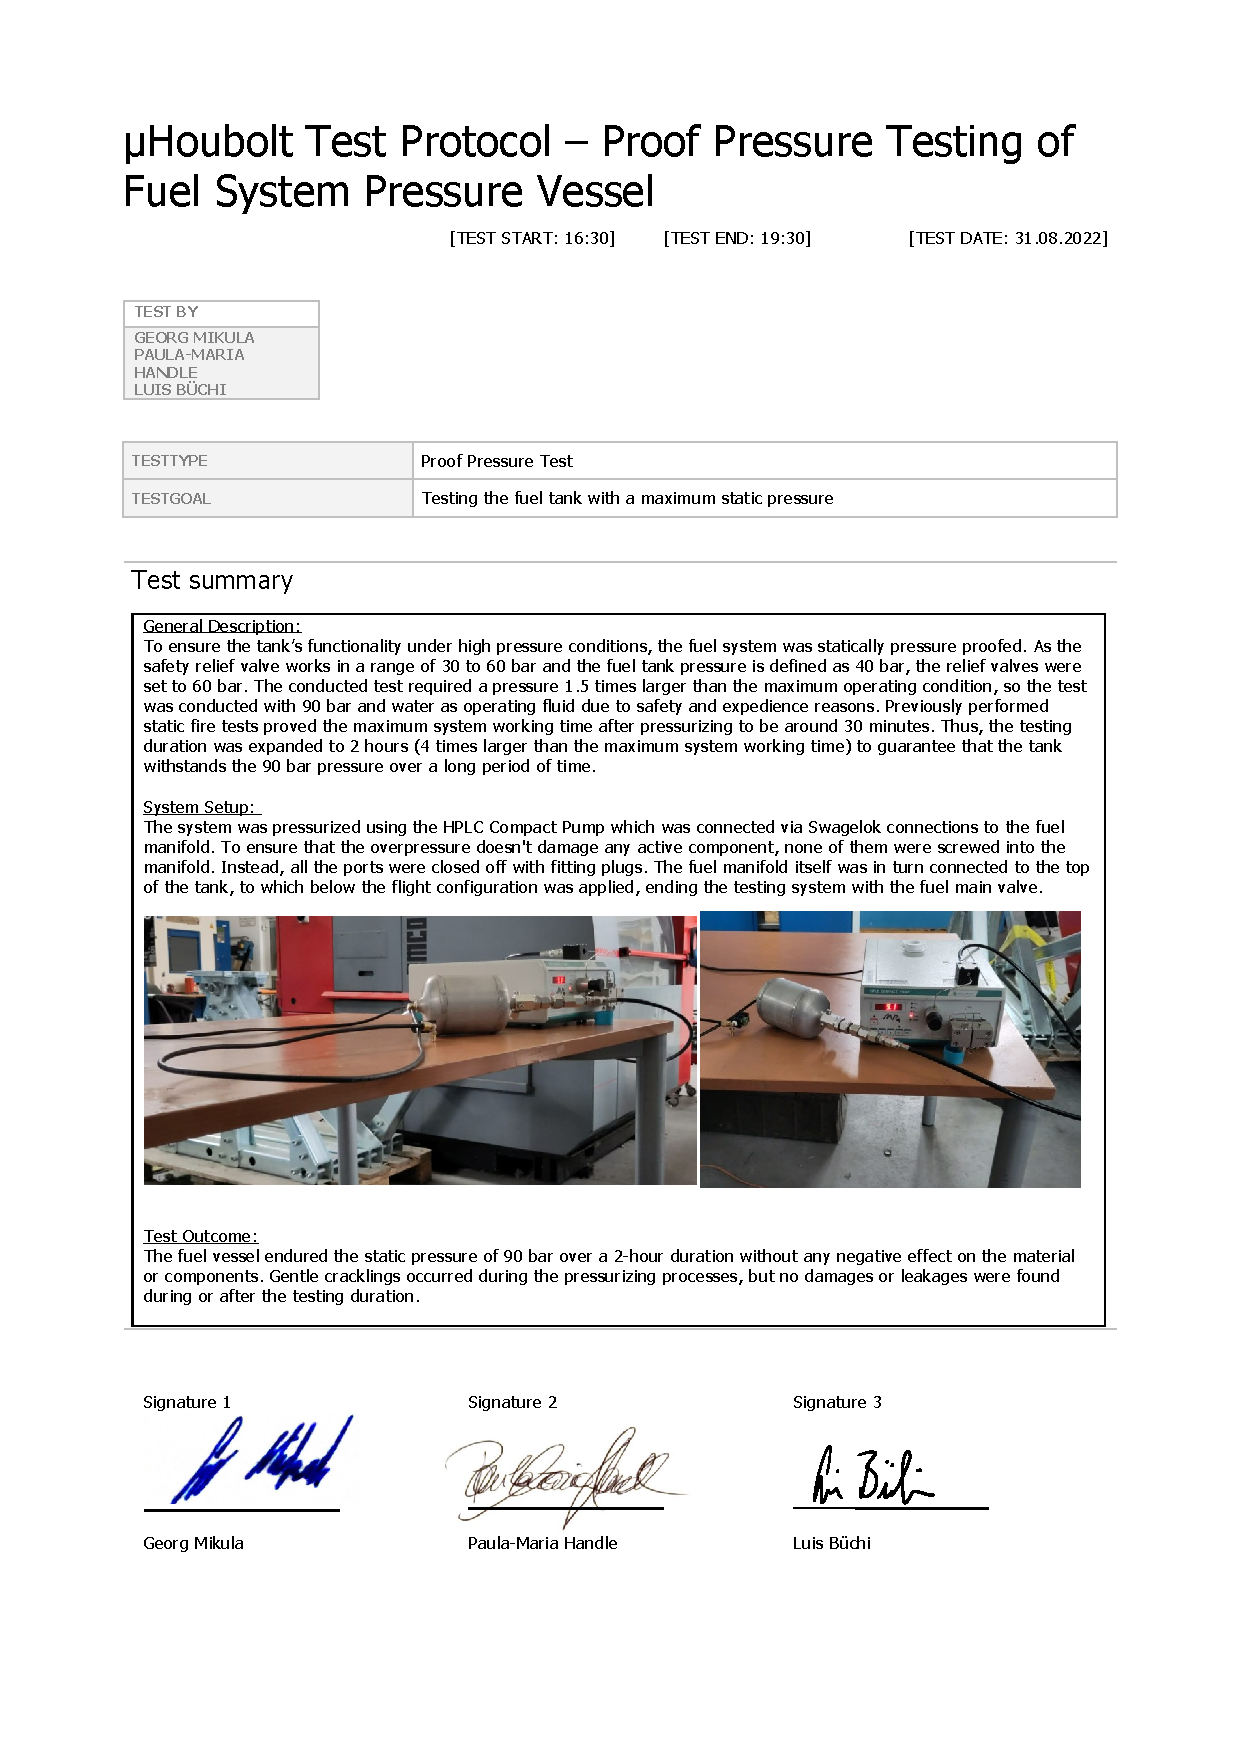
\includepdf[pages=-]{Appendices/uHoubolt_Proof_Pressure_Test_Fuel_Tank_signed.pdf}

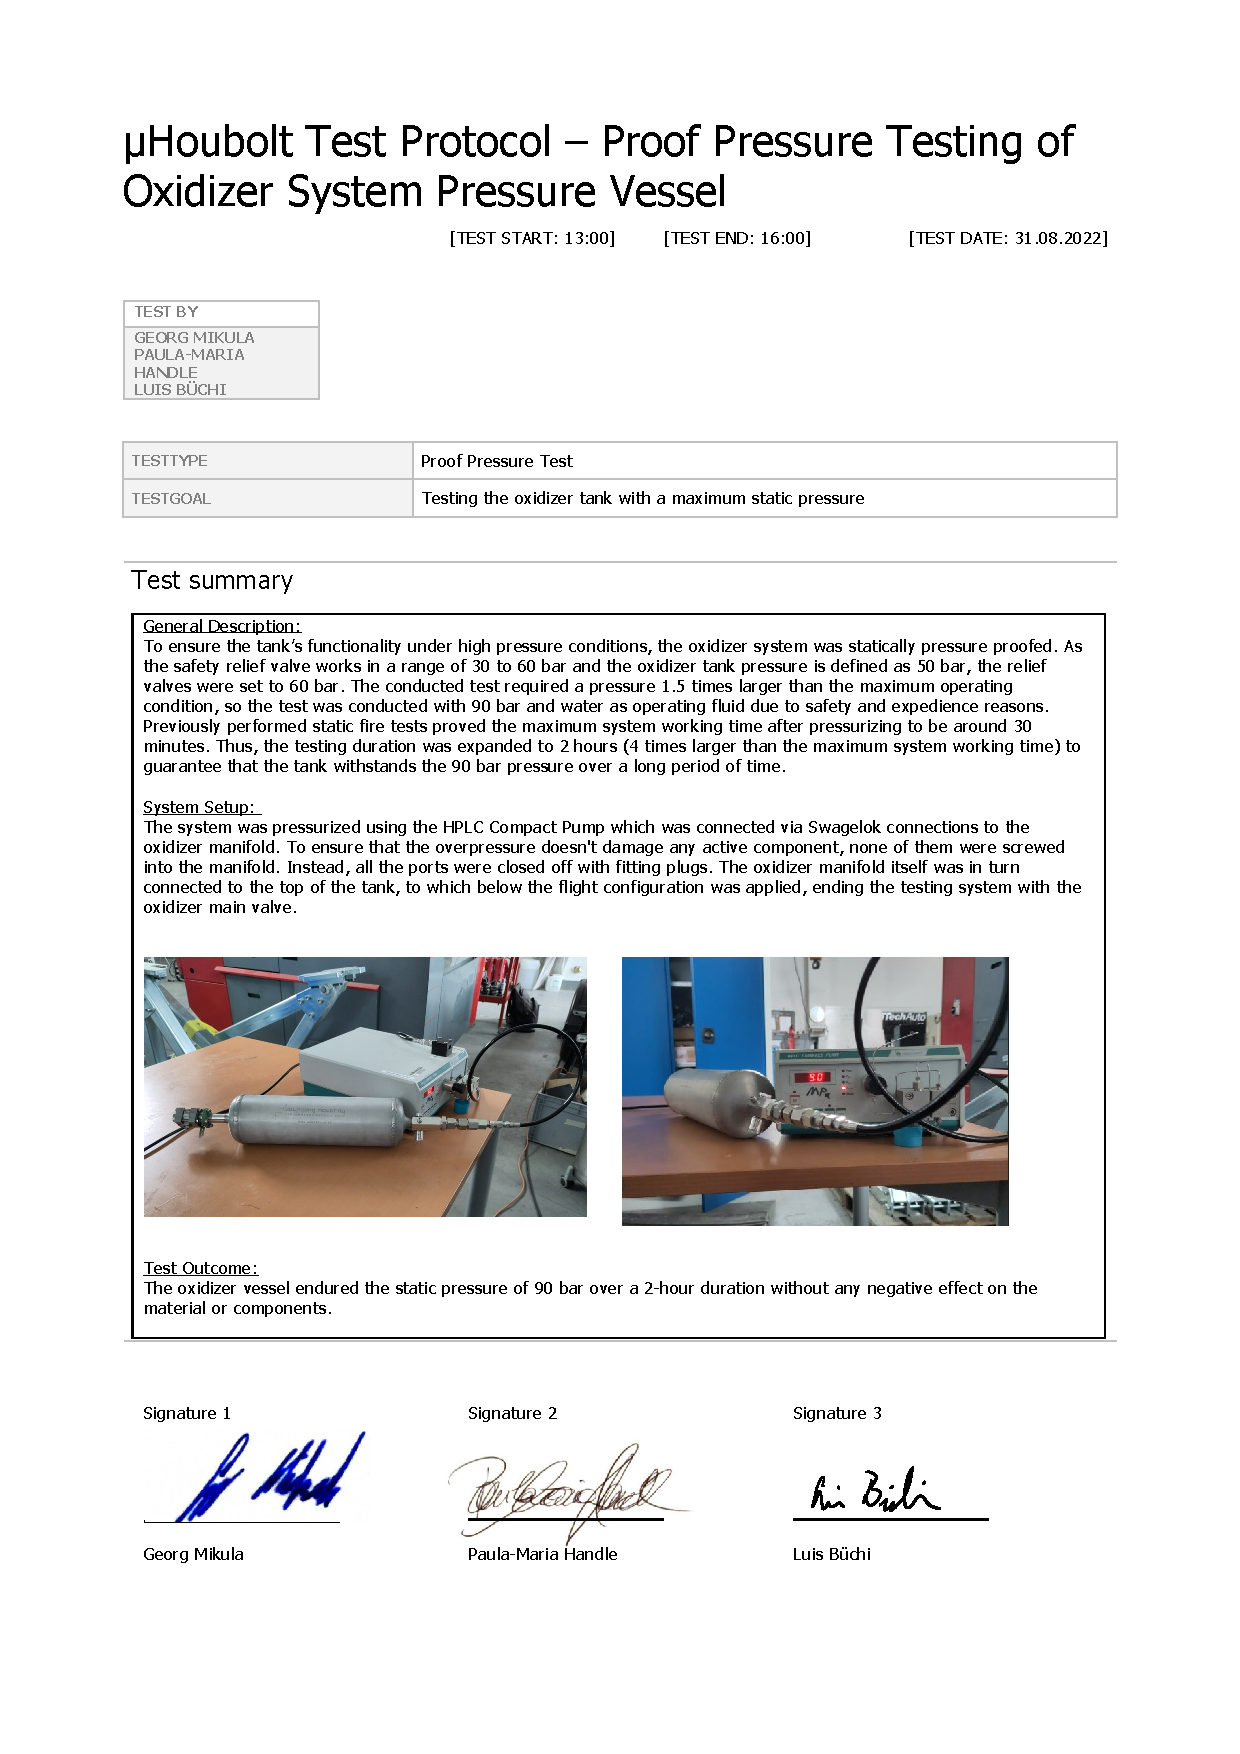
\includepdf[pages=-]{Appendices/uHoubolt_Proof_Pressure_Test_Ox_Tank_signed.pdf}

\subsection{Burst Pressure Testing Pressure Vessels}

THIS PAGE INTENTIONALLY LEFT BLANK

\newpage

\subsection{Test of SRAD flight computers with capability of actuating the recovery systems}

THIS PAGE INTENTIONALLY LEFT BLANK

\newpage

\section{Hazard Analysis Report}

\subsection{Liquid Propulsion System}

The liquid propulsion system contains by definition several hazardous materials and components:

\begin{itemize}
    \item Igniter
    \item Ethanol
    \item Nitrous Oxide
\end{itemize}

In the following the hazards related to these materials and the mitigations for them are laid out.

\begin{itemize}
    \item Transport
    \begin{itemize}
        \item \textbf{Igniter}
        
        Hazard: As the igniter is unsurprisingly flammable it poses a risk of starting to burn at an unwanted time. 
        
        Mitigation: The igniter mixture is put together on premise shortly before needing it, during transport the individual components are not dangerous.
        
        \item \textbf{Ethanol}
        
        Hazard: While not burning quickly, Ethanol is flammable and evaporates quickly.
        
        Mitigation: The ethanol gets transported and stored in their original packaging (plastic bottles).
        
        \item \textbf{Nitrous Oxide}
        
        Hazard: Tipping over could break the bottle open.
        
        Mitigation: Only gets transported with the safety lid on.
    \end{itemize}
\end{itemize}

\begin{itemize}
    \item Usage
    \begin{itemize}
        \item \textbf{Igniter}
        
        Hazard: Igniter going off after being installed on the combustion chamber or while being manufactured.
        
        Mitigation: The ignition system is only armed once the RBF pin is fully removed from the PMU, which happens just before launch preparations are done and the team vacates the launch pad. Before then, even on a misfire in the electronics, the igniter voltage to start the burning is physically disconnected. The person manufacturing the igniters wears eye protection and gloves. The heating plate is closely monitored to ensure proper heating temperature. All other people not involved hold their distance.
        
        \item \textbf{Ethanol}
        
        Hazard: Ethanol spills during handling could pose a fire risk on and around the pad.
        
        Mitigation: The ethanol gets filled into a large syringe away from the pad and then pushed from the syringe into the fuel tank. This removes potential spills from the pad.
        
        \item \textbf{Nitrous Oxide}
        
        Hazard: The nitrous oxide can explosively decompose.
        
        Mitigation: All parts that get in touch with the N2O get rigorously ox-cleaned. Filling the N2O tank in the rocket is one of the last steps of the launch checklist just before launch. Just one experienced member of personnel is at the launch rail. He/She opens the N2O gas cylinder. After some checks the last person leaves the launch rail. Only then the tanking of the N2O begins, controlled remotely from Mission Control. See \cref{sec:oxidizer_loading} for details on the oxidizer loading procedure.
    \end{itemize}
\end{itemize}

\subsection{Slingshot Mechanism in Recovery System}

Hazard: The slingshot mechanism of the recovery system stores considerable potential energy when loaded (See \cref{sec:recovery}). During launch preparations this has to be done a while before the pad crew vacates the premises and as such the slingshot mechanism could (mis)fire when personnel is around. This could happen if the knot loosens or the recovery system fails and prematurely detects apogee on the pad.

Mitigation: As soon as the mechanism is loaded a cable tie gets wrapped around the clampband which stops the mechanism from firing until removed right before the crew leaves the launch pad.

\section{Risk Assessment}

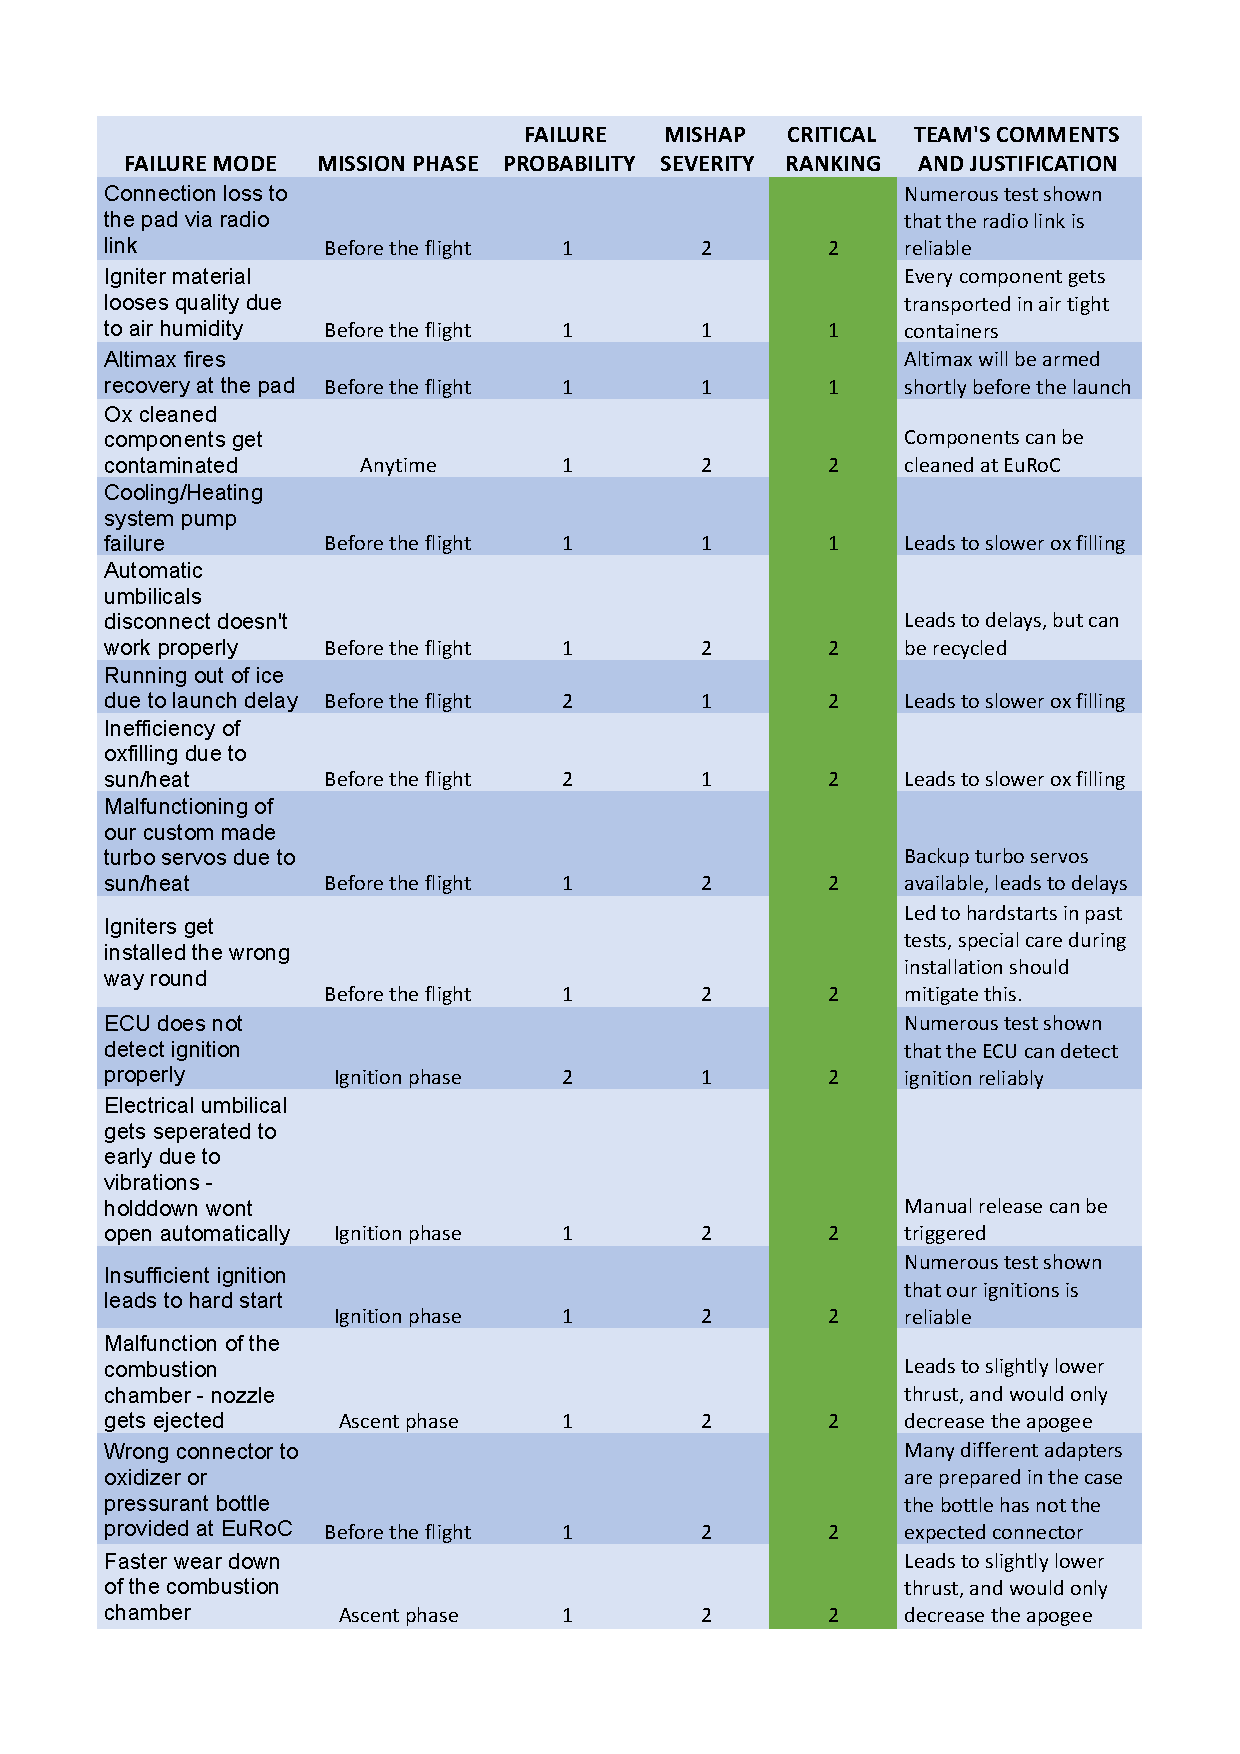
\includepdf[pages=-]{Appendices/RiskAssessment.pdf}

\section{Checklists}

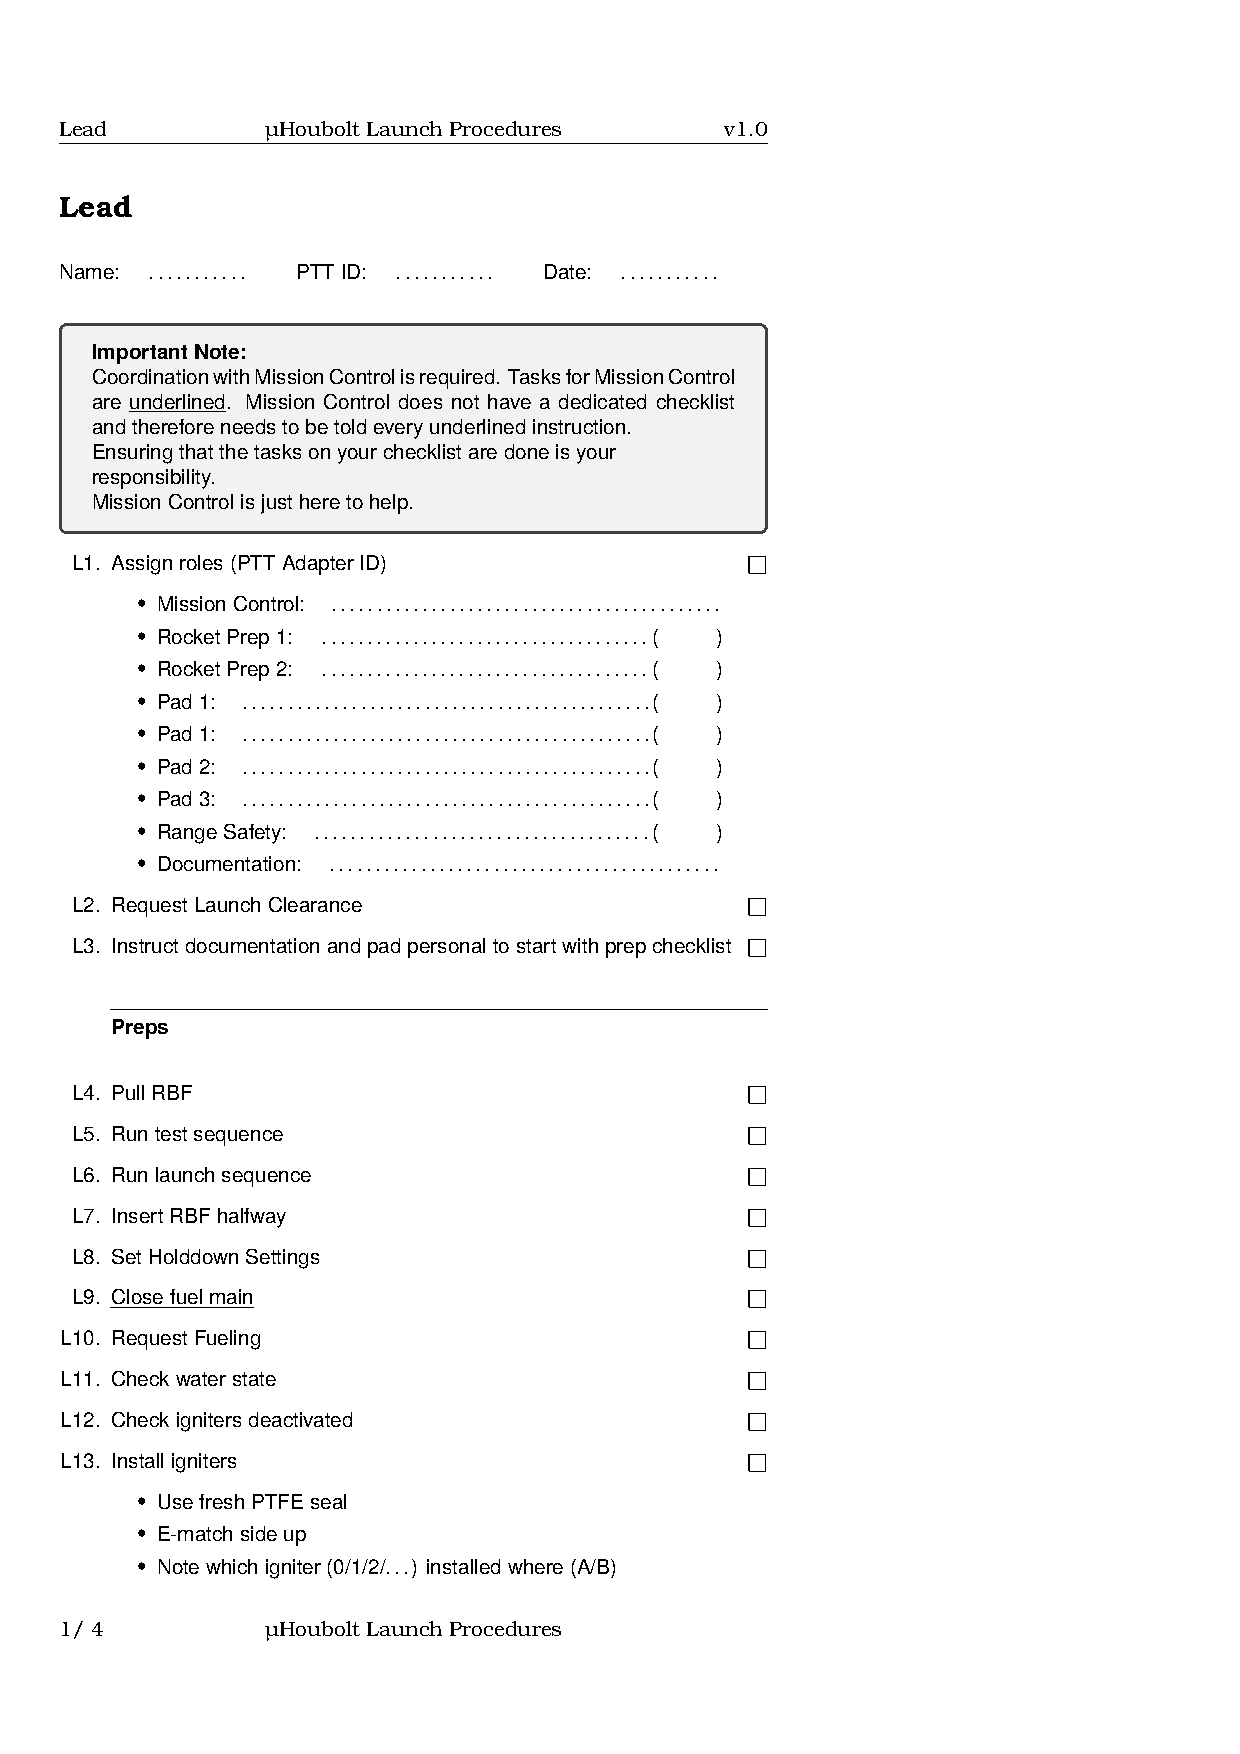
\includepdf[pages={1-6}]{Appendices/Houbolt_Launch_Procedures.pdf}

\section{Engineering Drawings}

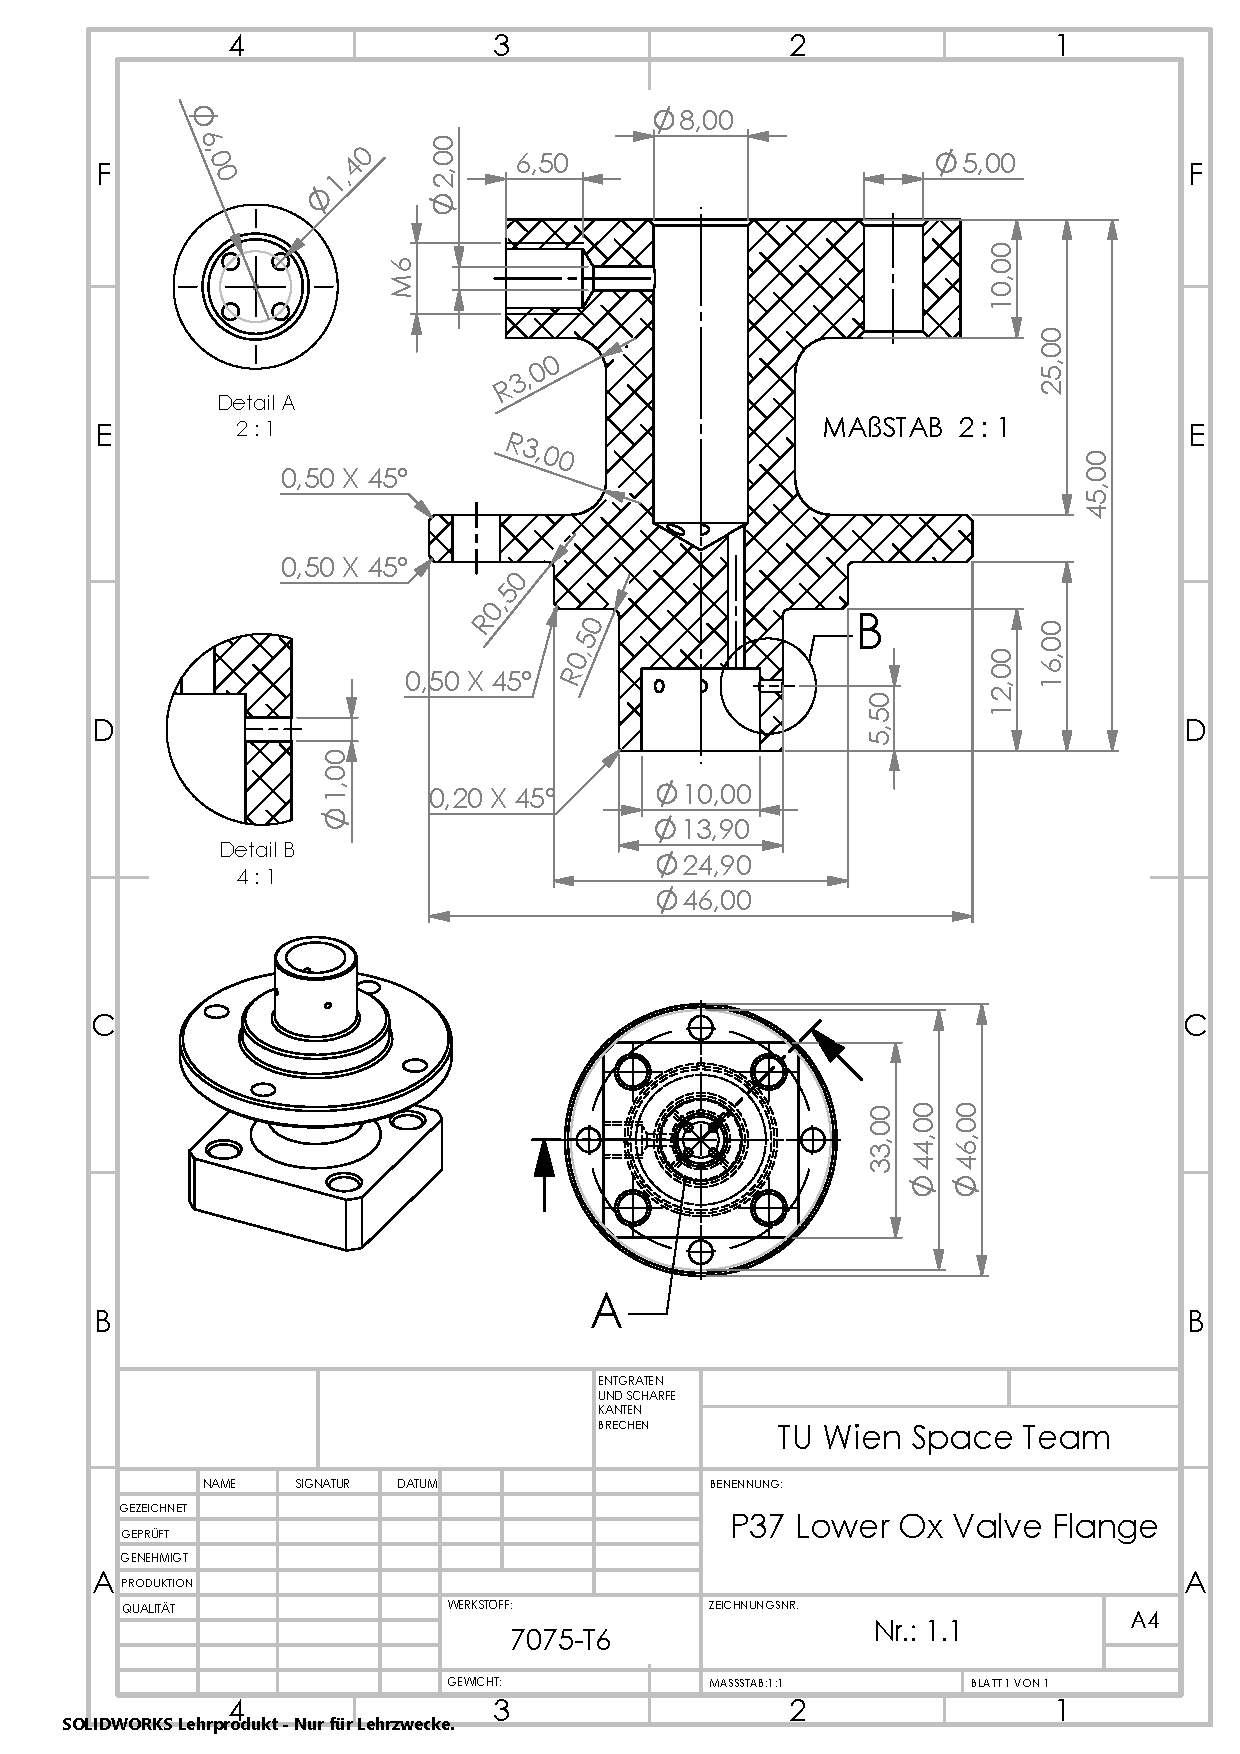
\includepdf[pages=-]{Appendices/P37_Injector_Lower_Ox_Valve_Flange.pdf}
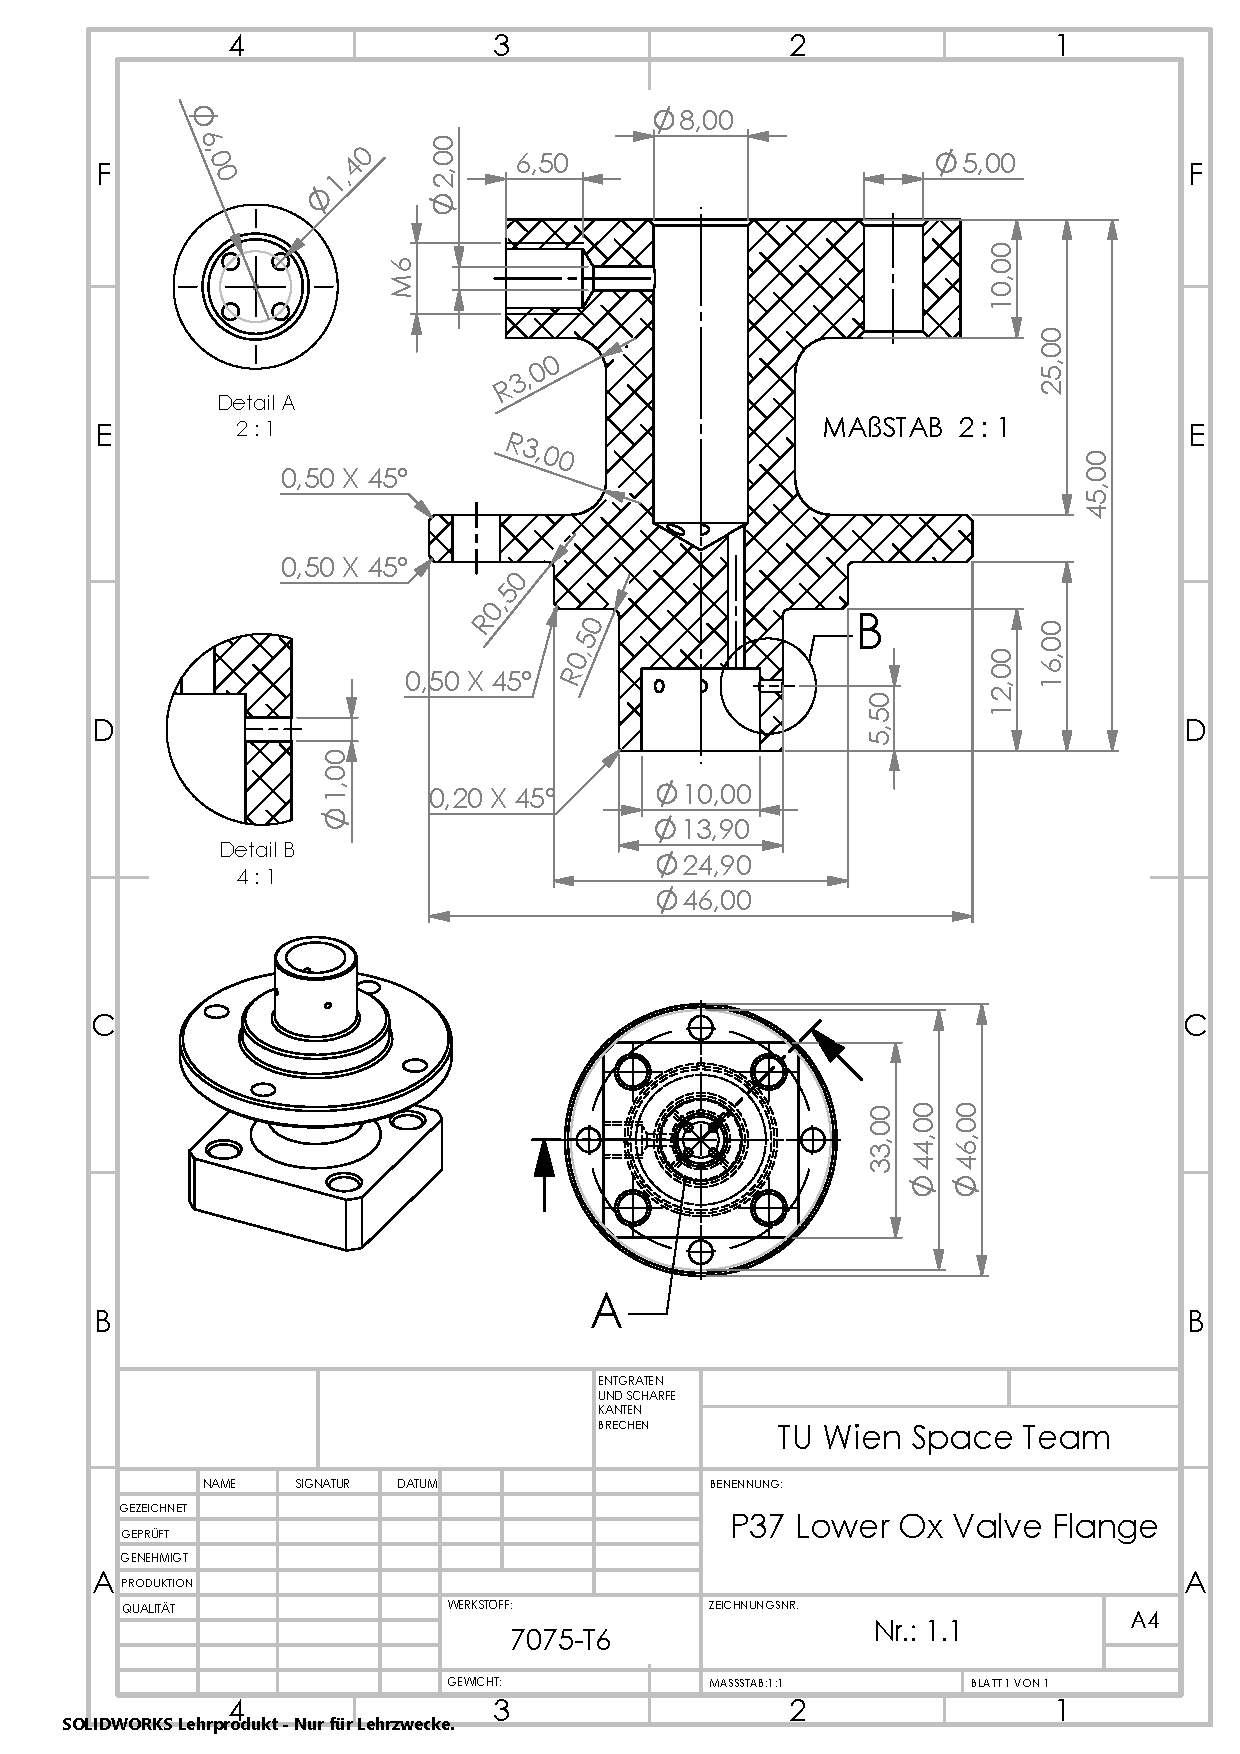
\includepdf[pages=-]{Appendices/P37_Lower_Ox_Valve_Flange.pdf}
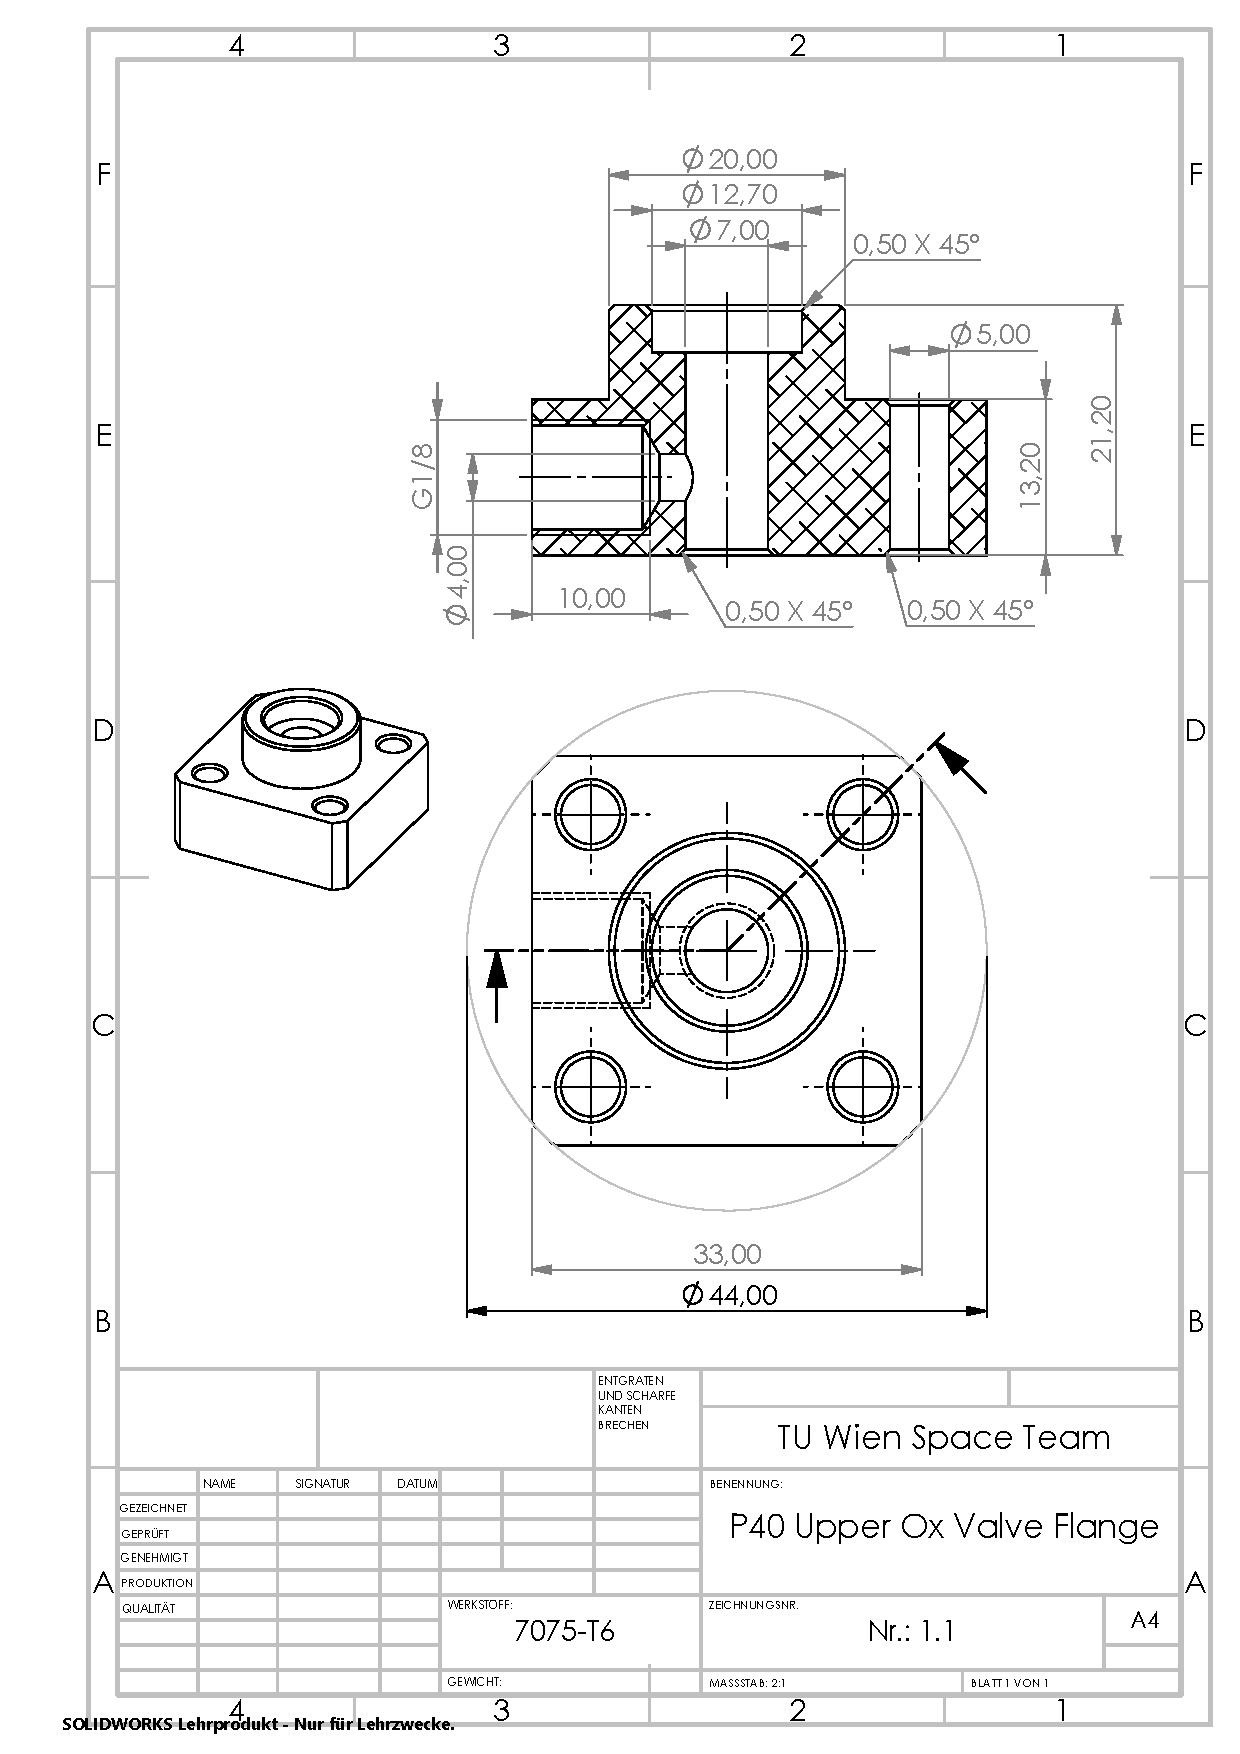
\includepdf[pages=-]{Appendices/P40_Upper_Ox_Valve_Flange.pdf}
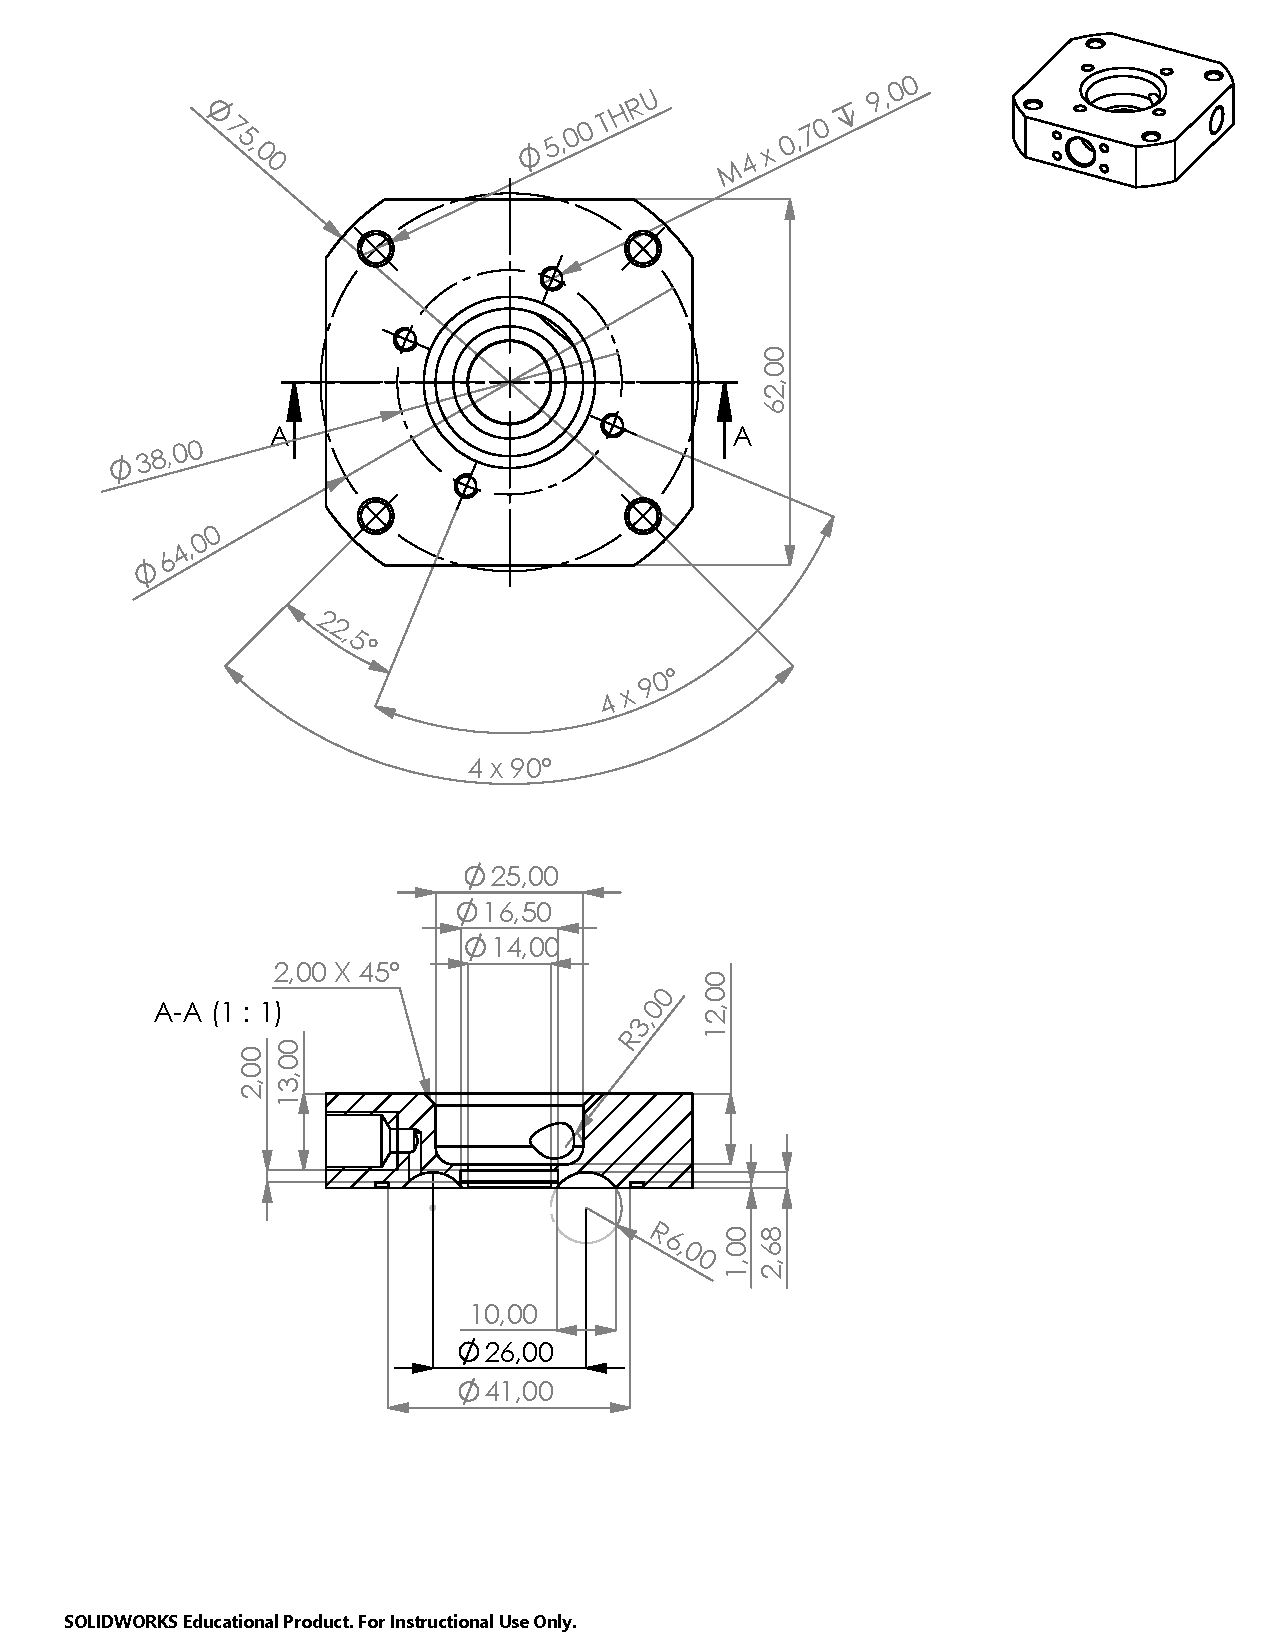
\includepdf[pages=-]{Appendices/EngineHead.pdf}
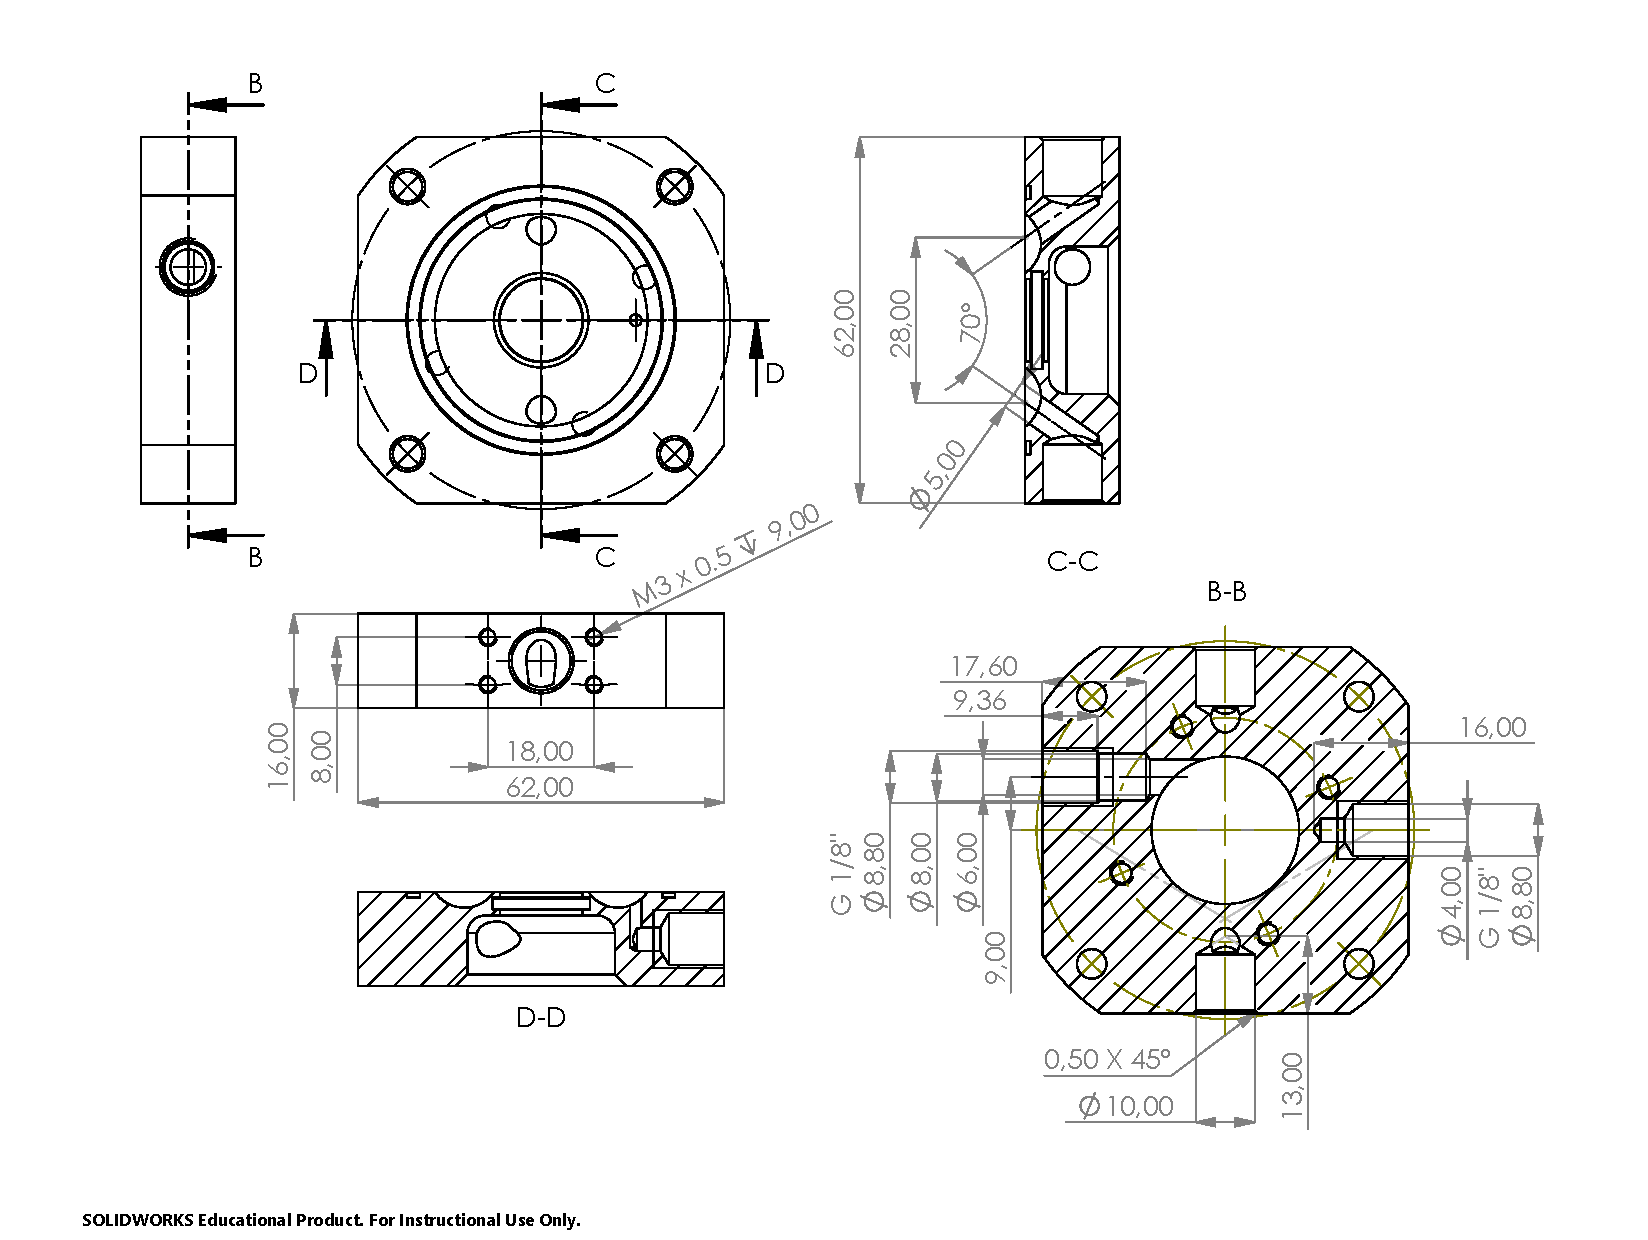
\includepdf[pages=-]{Appendices/EngineHead2.pdf}

%from here on out optional
\section{Detailed Software Architecture}\label{sec:software}

\begin{figure}[h]
    \centering
    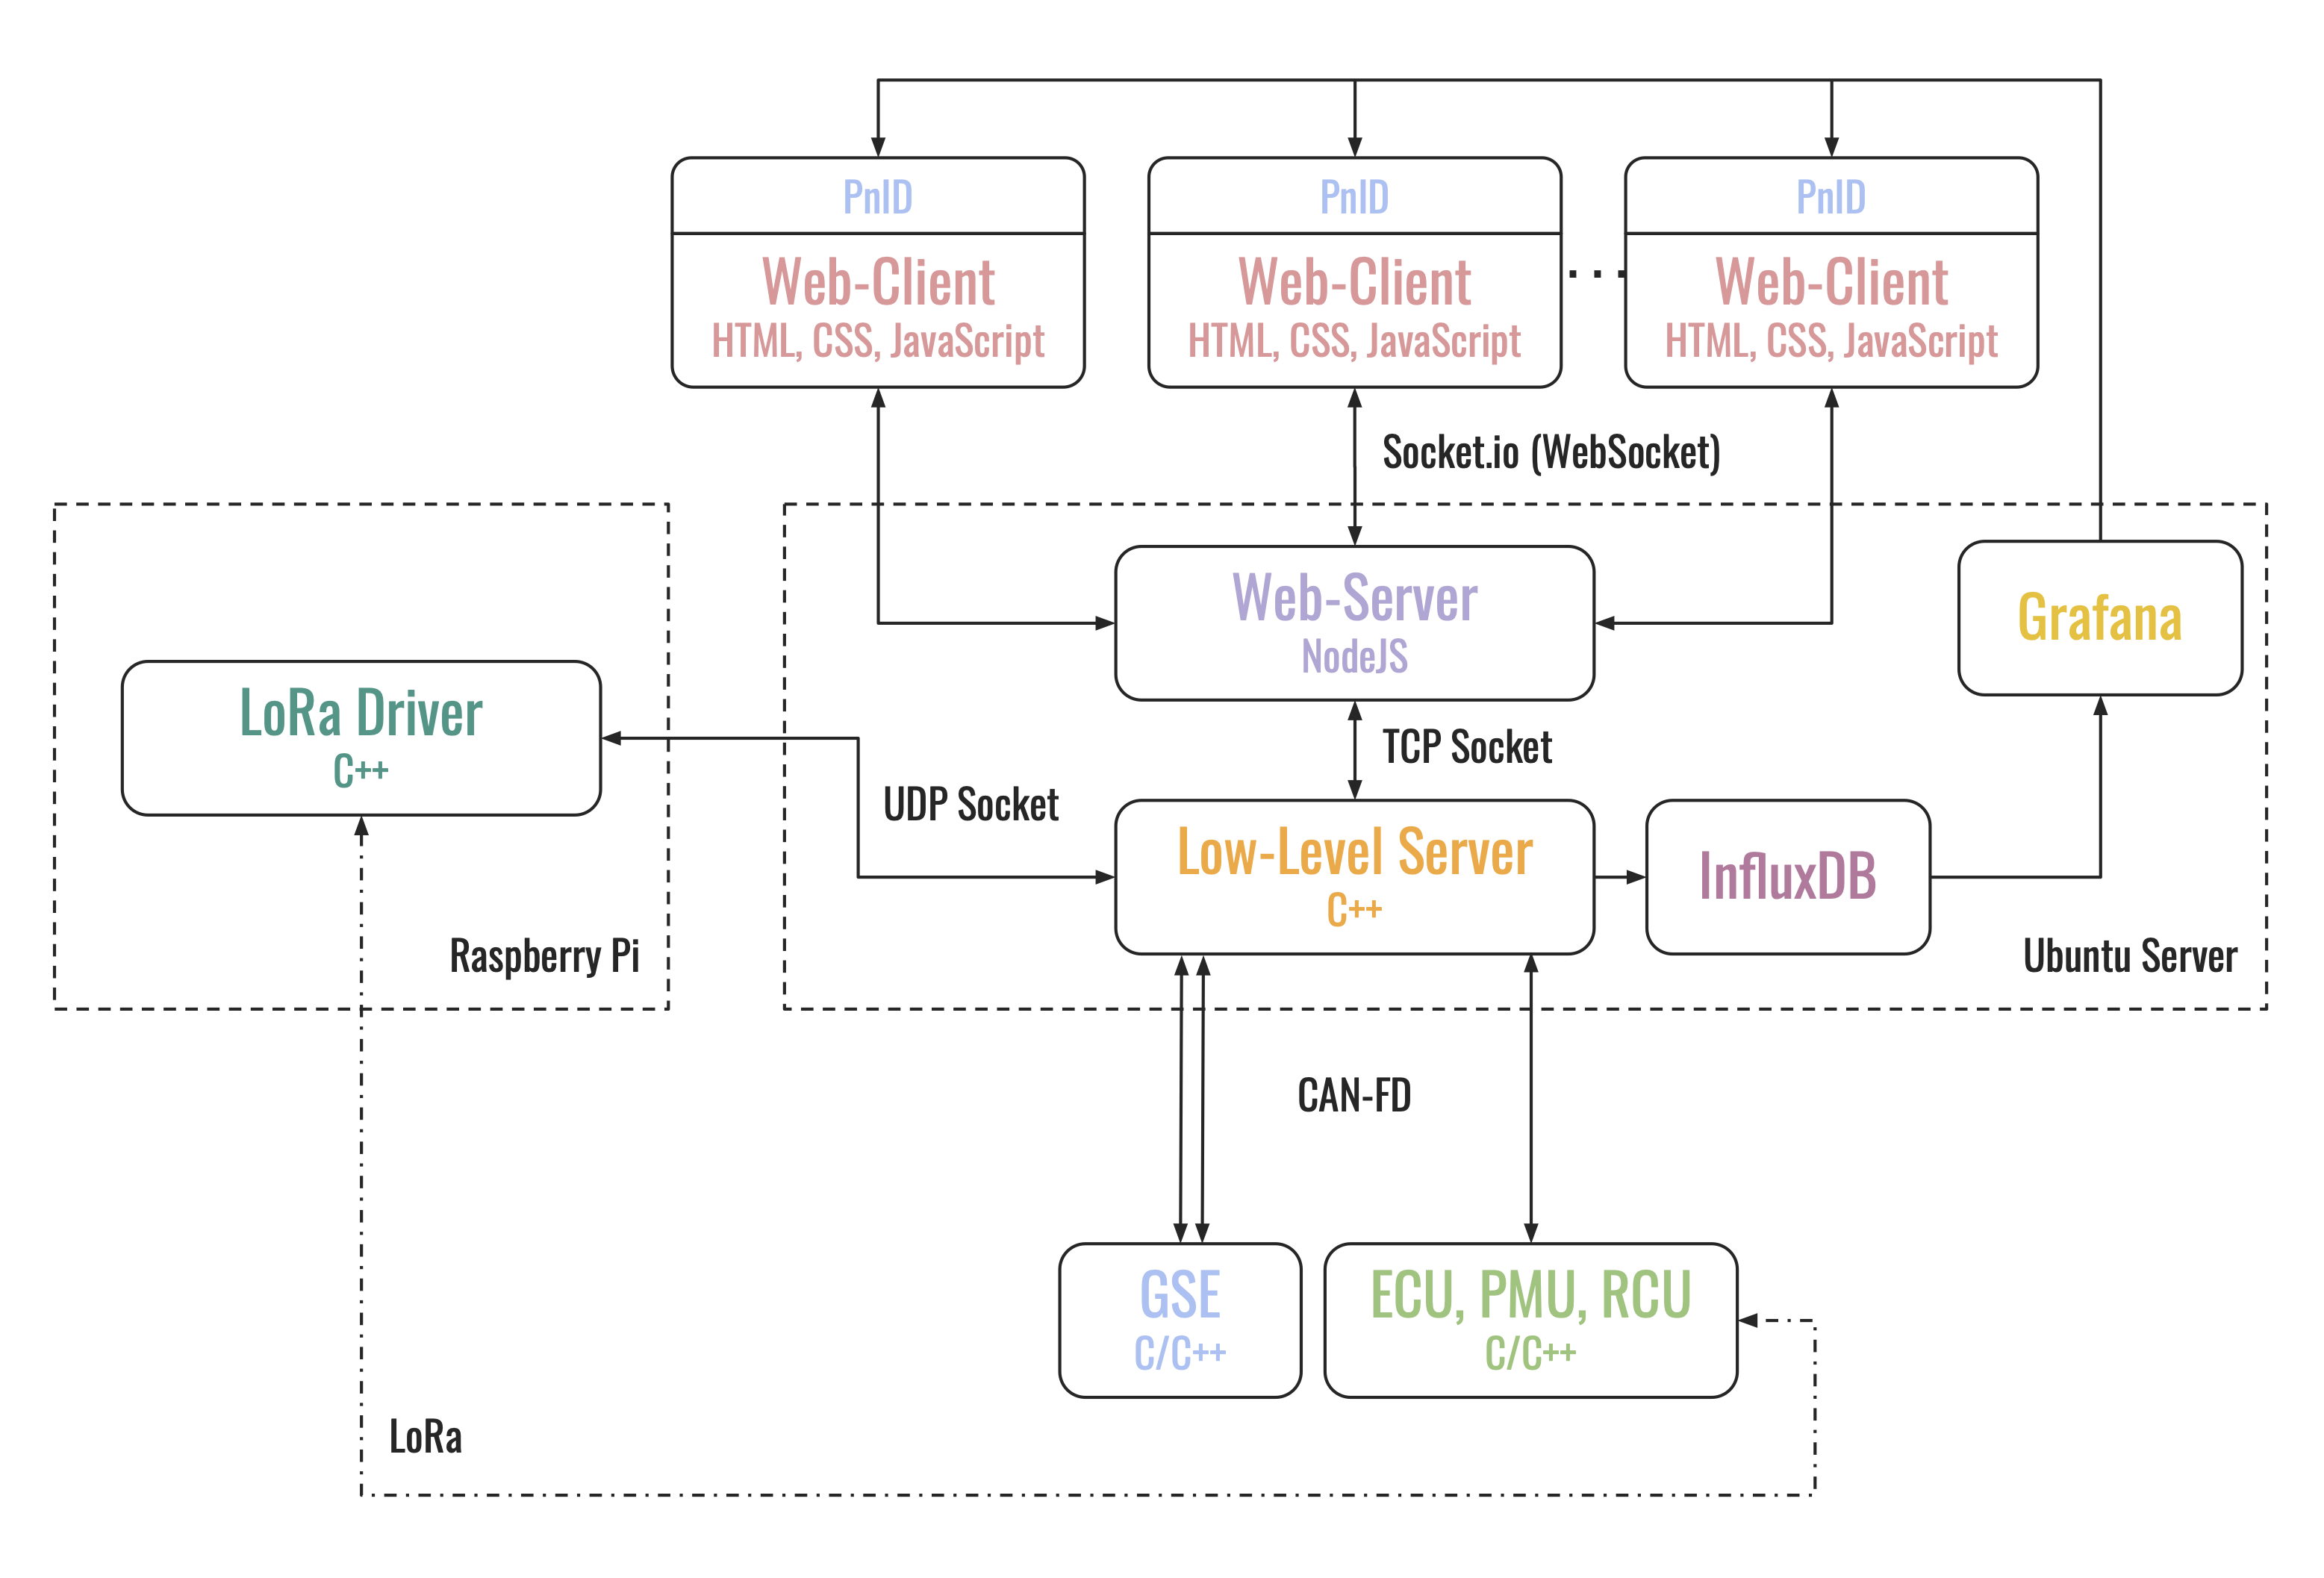
\includegraphics[width=0.7\textwidth]{Appendices/Software Architecture.png}
    \caption{Software Architecture}
    \label{fig:software}
\end{figure}


\subsection{Mission Control} %Markus
Mission Control consists of a PC or Laptop running a Web-Application (Web-Client) inside a Web-Browser. It manages the communication between the Operator and the Rocket as well as the Ground Support Equipment. The Web-Client displays all measured data and actuators in a self developed interactive Piping and Instrumentation Diagram (P\&ID/PnID). 
Every value for each P\&ID element gets validated. When out of range, it is
signalled by changing colour. This way, the operator doesn't have to check
each number in detail but rather only has to watch for color changes, which is much
more apparent.

\subsection{Ubuntu Server}

The Ubuntu Server uses a PCIe CAN bus extension card with four CAN bus ports.
It is responsible for communication with the Hardware, i.e. GSE, ECU, RCU and PMU.
Mission Control interfaces with the Hardware via a self developed software as 
depicted in figure \ref{fig:software}. The connection from the server to Mission Control can either be made by a long Ethernet cable or a directed radio link depending on the necessary safety distance of MC from the pad. 

\paragraph{Low-Level Server}

Written in C++ it is responsible for managing CAN and other time critical tasks such as logging and processing sensor data.

\paragraph{Web-Server}

Uses NodeJS to host the Web-Clients and synchronize data between them.

\paragraph{InfluxDB and Grafana}

InfluxDB is a time series based database for logging sensor data and user inputs. Grafana is used for real time plots and gauges on the Web-Client. It is also used for
post-launch procedures.

\subsection{LoRa Raspberry Pi}

To communicate with the rocket during flight, LoRa is used. A self developed
LoRa transceiver shield is connected to a Raspberry Pi which processes and 
transmits the messages over UDP to the Ubuntu Server. There it gets processed
like a normal CAN Message.


\newpage

\renewcommand{\bibname}{References}
\bibliographystyle{plain}
\bibliography{references}

\end{document}
